% BU ECE template for MS thesis and PhD dissertation.
%
%==========================================================================%
% MAIN PREAMBLE 
%==========================================================================%
\documentclass[12pt,letterpaper]{report}          % Single-sided printing for the library
%\documentclass[12pt,twoside]{report} % Double-sided printing
\usepackage[intlimits]{amsmath}
\usepackage{amsfonts,amssymb}
\DeclareSymbolFontAlphabet{\mathbb}{AMSb}
%\usepackage{natbib}
\usepackage{apalike}
\usepackage{multirow}
\usepackage{float}
\usepackage[bf]{caption}       
\setcaptionmargin{0.5in}
\usepackage{fancyhdr}
%\usepackage{fancyheadings}
\usepackage{fancybox}
\usepackage{ifthen}
\usepackage{bu_ece_thesis}
\usepackage{url}
\usepackage{lscape,afterpage}
\usepackage{xspace}
\usepackage{epstopdf} 
\usepackage{subfig}
\usepackage[lined,ruled]{algorithm2e}
\usepackage{listings}
\lstset{
    %frame=single,
    frame=L,
    basicstyle=\footnotesize,
    breaklines=true,
    %postbreak=\raisebox{0ex}[0ex][0ex]{\ensuremath{\color{red}\hookrightarrow\space}}
}
\lstdefinelanguage{scad}{
    keywords = {
        chip,Wc,Hc,YPos,
	for,let,translate,len,module
    },
}
%==========================================================================%
%%% graphicx and pdf creation
\usepackage{graphicx}
\usepackage{appendix}
%\usepackage{psfrag}
%\DeclareGraphicsExtensions{.eps}   % extension for included graphics
%\usepackage{thumbpdf}              % thumbnails for ps2pdf
%\usepackage[ps2pdf,                % hyper-references for ps2pdf
%bookmarks=true,%                   % generate bookmarks ...
%bookmarksnumbered=true,%           % ... with numbers
%hypertexnames=false,%              % needed for correct links to figures !!!
%breaklinks=true,%                  % breaks lines, but links are very small
%linkbordercolor={0 0 1},%          % blue frames around links
%pdfborder={0 0 112.0}]{hyperref}%  % border-width of frames 
%                                   % will be multiplied with 0.009 by ps2pdf
%\hypersetup{
%  pdfauthor   = {Joe Graduate <joe.graduate@bu.edu>},
%  pdftitle    = {dissertation.pdf},
%  pdfsubject  = {doctoral dissertations},
%  pdfkeywords = {mathematics, science, technology},
%  pdfcreator  = {LaTeX with hyperref package},
%  pdfproducer = {dvips + ps2pdf}
%}
%==========================================================================%
% customized commands can be placed here
%\newcommand{\figref}[1]{Figure~\ref{#1}}
%\newcommand{\chapref}[1]{Chapter~\ref{#1}}
%\newcommand{\latex}{\LaTeX\xspace}
%==========================================================================%

%==========================================================================%
% BEGIN
%==========================================================================%
\begin{document}

% The preliminary pages
% This file contains all the necessary setup and commands to create
% the preliminary pages according to the buthesis.sty option.

\title{MakerFluidics: Low Cost Microfluidics for Synthetic Biology}

\author{Ryan Silva}

% Type of document prepared for this degree:
%   1 = Master of Science thesis,
%   2 = Doctor of Philisophy dissertation.
%   3 = Master of Science thesis and Doctor of Philisophy dissertation.
\degree=2

\prevdegrees{B.S., United States Air Force Academy, 2005\\
	M.S., The Air Force Institute of Technology, 2007}

\department{Department of Electrical and Computer Engineering}

% Degree year is the year the diploma is expected, and defense year is
% the year the dissertation is written up and defended. Often, these
% will be the same, except for January graduation, when your defense
% will be in the fall of year X, and your graduation will be in
% January of year X+1
\defenseyear{2017}
\degreeyear{2017}

% For each reader, specify appropriate label {First, Second, Third},
% then name, and title. IMPORTANT: The title should be:
%   "Professor of Electrical and Computer Engineering",
% or similar, but it MUST NOT be:
%   Professor, Department of Electrical and Computer Engineering"
% or you will be asked to reprint and get new signatures.
% Warning: If you have more than five readers you are out of luck,
% because it will overflow to a new page. You may try to put part of
% the title in with the name.
\reader{First}{Douglas M. Densmore, Ph.D.}{Associate Professor of Electrical and Computer Engineering \\ Associate Professor of Biomedical Engineering}
\reader{Second}{Jason W. Holder, Ph.D.}{Principal Member, Technical Staff \\ The Charles Stark Draper Laboratory, Inc.}
\reader{Third}{Ajay Joshi, Ph.D.}{Associate Professor of Electrical and Computer Engineering}
\reader{Fourth}{Michel Kinsy, Ph.D.}{Assistant Professor of Electrical and Computer Engineering}
\reader{Fifth}{James Galagan, Ph.D.}{Associate Professor of Biomedical Engineering \\ Boston University, College of Engineering \vspace{6pt}\\ Associate Professor of Microbiology \\ Boston University, School of Medicine}

% The Major Professor is the same as the first reader, but must be
% specified again for the abstract page. Up to 4 Major Professors
% (advisors) can be defined. 
\numadvisors=2
\majorprof{Douglas M. Densmore, Ph.D.}{{Associate Professor of Electrical and Computer Engineering \\ Associate Professor of Biomedical Engineering}}
%\majorprof{Douglas Densmore, Ph.D.}{{Associate Professor of Electrical and Computer Engineering}}
\majorprofb{Jason W. Holder, Ph.D.}{{Principal Member, Technical Staff \\ The Charles Stark Draper Laboratory, Inc.}}
%\majorprofb{Jason W. Holder, PhD}{{Principal Member of Technical Staff, The Charles Stark Draper Laboratory}}
%\majorprofc{First M. Last, PhD}{{Professor of Astronomy}}
%\majorprofd{First M. Last, PhD}{{Professor of Biomedical Engineering}}

%%%%%%%%%%%%%%%%%%%%%%%%%%%%%%%%%%%%%%%%%%%%%%%%%%%%%%%%%%%%%%%%  

%                       PRELIMINARY PAGES
% According to the BU guide the preliminary pages consist of:
% title, copyright (optional), approval,  acknowledgments (opt.),
% abstract, preface (opt.), Table of contents, List of tables (if
% any), List of illustrations (if any). The \tableofcontents,
% \listoffigures, and \listoftables commands can be used in the
% appropriate places. For other things like preface, do it manually
% with something like \newpage\section*{Preface}.

% This is an additional page to print a boxed-in title, author name and
% degree statement so that they are visible through the opening in BU
% covers used for reports. This makes a nicely bound copy. Uncomment only
% if you are printing a hardcopy for such covers. Leave commented out
% when producing PDF for library submission.
%\buecethesistitleboxpage

% Make the titlepage based on the above information.  If you need
% something special and can't use the standard form, you can specify
% the exact text of the titlepage yourself.  Put it in a titlepage
% environment and leave blank lines where you want vertical space.
% The spaces will be adjusted to fill the entire page.
\maketitle
\cleardoublepage

% The copyright page is blank except for the notice at the bottom. You
% must provide your name in capitals.
\copyrightpage
\cleardoublepage

% Now include the approval page based on the readers information
\approvalpage
\cleardoublepage

% Here goes your favorite quote. This page is optional.
\newpage
%\thispagestyle{empty}
\phantom{.}
\vspace{4in}

\begin{singlespace}
\begin{quote}
  \textit{Shout out to Jesus}
\end{quote}
\end{singlespace}

% \vspace{0.7in}
%
% \noindent
% [The descent to Avernus is easy; the gate of Pluto stands open night
% and day; but to retrace one's steps and return to the upper air, that
% is the toil, that the difficulty.]

\cleardoublepage

% The acknowledgment page should go here. Use something like
% \newpage\section*{Acknowledgments} followed by your text.
\newpage
\section*{\centerline{Acknowledgments}}
I would like to first thank my amazing, beautiful wife who puts up with my nonsense. Shout out to Baby Jay, even though he was a late arrival to this party. When I come home from a long day at the lab and see the smile on his little face, I just know he's about to jab me with something.

There is no better PhD advisor than Douglas Densmore. He taught me the one little word that will get me through academic life and beyond: \emph{tranquillo}. Like me, he understands that sometimes in life you only get to order one \emph{primi} [sic]. In all seriousness, I have yet to describe my PhD experience to anyone without inducing some serious PI envy. Thank you for everything and I will cherish the days you allowed me to spend in your lab. Thanks to the Fluigi crew (Josh, Krishna, Ali) and Prashant for always getting me home safe and on-time.

Special thanks to Jason Holder, who pushed me to develop a thesis of which I can be proud. Thank you for letting me be a part of your lab and your team. What can I say about the Acoustic Boyz? Thanks to Parker Dow for teaching me everything I know; thanks to Charlie Lissandrello for the dusty lemonade; apologies to Ryan Dubay, I blame it on the economy; thanks to Ken ``Doctor'' Kotz for your curiosity in my project by always asking if it's working; thanks to Peter, David, Chris and Helen for granting me four square feet in the productivity hub known simply as ``The Pitt''; thanks to Jac, Sarah, and Sammy G. for staying up until 4am on a work night; thanks to Jason Fiering for allowing me to distract his best workers.


Shout out to my funding agency and my employer, the United States Air Force, where, maybe, just once, someone will call me ``Sir'' without adding, ``You're making a scene.''

\cleardoublepage

% The abstractpage environment sets up everything on the page except
% the text itself.  The title and other header material are put at the
% top of the page, and the supervisors are listed at the bottom.  A
% new page is begun both before and after.  Of course, an abstract may
% be more than one page itself.  If you need more control over the
% format of the page, you can use the abstract environment, which puts
% the word "Abstract" at the beginning and single spaces its text.

\begin{abstractpage}
Recent advancements in multilayer, multicellular, genetic logic circuits often rely on manual intervention throughout the computation cycle and orthogonal signals for each chemical ``wire''. These constraints can prevent genetic circuits from scaling. Microfluidic devices can be used to mitigate these constraints. However, continuous-flow microfluidics are largely designed through artisanal processes involving hand-drawing features and accomplishing design rule checks visually: processes that are also inextensible. Additionally, continuous-flow microfluidic routing is only a consideration during chip design and, once built, the routing structure becomes ``frozen in silicon,'' or for many microfluidic chips ``frozen in polydimethylsiloxane (PDMS)''; any changes to fluid routing often require an entirely new device and control infrastructure. The cost of fabricating and controlling a new device is high in terms of time and money; attempts to reduce one cost measure are, generally, paid through increases in the other. 

This work has three main thrusts: to create a microfluidic fabrication framework, called MakerFluidics, that lowers the barrier to entry for designing and fabricating microfluidics in a manner amenable to automation (Chapter \ref{chapter:mf}); to prove this methodology can design, fabricate, and control complex and novel microfluidic devices (Chapter \ref{chapter:xposer}); and to demonstrate the methodology can be used to solve biologically-relevant problems (Chapter \ref{chapter:acoust}).

Utilizing accessible technologies, rapid prototyping, and scalable design practices, the MakerFluidics framework has demonstrated its ability to design, fabricate and control novel, complex and scalable microfludic devices. This was proven through the development of a reconfigurable, continuous-flow routing fabric driven by a modular, scalable primitive called a transposer. In addition to creating complex microfluidic networks, MakerFluidics was deployed in support of cutting-edge, application-focused research at the Charles Stark Draper Laboratory. Informed by a design of experiments approach using the parametric rapid prototyping capabilities made possible by MakerFluidics, a plastic blood--bacteria separation device was optimized, demonstrating that the new device geometry can separate bacteria from blood while operating at 275\% greater flow rate as well as reduce the power requirement by 82\% for equivalent separation performance when compared to the state of the art. 

Ultimately, MakerFluidics demonstrated the ability to design, fabricate, and control complex and practical microfluidic devices while lowering the barrier to entry to continuous-flow microfluidics, thus democratizing cutting edge technology beyond a handful of well-resourced and specialized labs. 


%This research addresses each of the above issues in turn by applying lessons learned from the evolution of electronic computation, ultimately resulting in a microfluidic fabrication and control paradigm called MakerFluidics. Automation via computer aided design (CAD) and computer aided manufacturing (CAM) is stressed through the use of algorithmic frameworks, accessible technologies, rapid prototyping, and scalable design practices. These efforts are focused towards lowering the barrier to entry for continuous-flow microfluidics, thus democratizing the utilization of cutting edge technology beyond a handful of well-resourced and specialized labs. This can only be accomplished by viewing accessibility as a constraint to development.

\end{abstractpage}
\cleardoublepage

% Now you can include a preface. Again, use something like
% \newpage\section*{Preface} followed by your text

% Table of contents comes after preface
\tableofcontents
\cleardoublepage

% If you do not have tables, comment out the following lines
\newpage
\listoftables
\cleardoublepage

% If you have figures, uncomment the following line
\newpage
\listoffigures
\cleardoublepage

% List of Abbrevs is NOT optional (Martha Wellman likes all abbrevs listed)
\chapter*{List of Abbreviations}
\begin{center}
  \begin{tabular}{lll}
    \hspace*{2em} & \hspace*{1in} & \hspace*{4.5in} \\
    ASIC & \dotfill & Application Specific Integrated Circuit \\
    CAD  & \dotfill & Computer-Aided Design \\
    CAM  & \dotfill & Computer-Aided Manufacturing \\
    FWHM & \dotfill & Full-Width at Half Maximum \\
    IDAST &\dotfill & Identification and Antibiotic Susceptibility Test\\
    mLSI & \dotfill & Microfluidic Large Scale Integration \\
    PCB  & \dotfill & Printed Circuit Board \\
    PDMS & \dotfill & Polydimethylsiloxane \\
    $\mathbb{R}^{2}$  & \dotfill & the Real plane \\
    UV	 & \dotfill & Ultra-Violet \\
    VLSI & \dotfill & Very Large Scale Integration \\
  \end{tabular}
\end{center}
\cleardoublepage

% END OF THE PRELIMINARY PAGES

\newpage
\endofprelim
        
\cleardoublepage

% -------------------------------------
% CHAPTER 1: INTRODUCTION
% -------------------------------------
\chapter{Introduction}
\label{chapter:Introduction}
\thispagestyle{myheadings}

%This work has three main thrusts: to create a microfluidic fabrication framework that lowers the barrier to entry for designing and fabricating microfluidics in a manner amenable to automation (Chapter \ref{chapter:mf}); to prove this methodology can design, fabricate, and control complex and novel microfluidic devices (Chapter \ref{chapter:xposer}); and to demonstrate the methodology can be used to solve biologically-relevant problems (Chapter \ref{chapter:acoust}).

Cellular computation is necessary for the orchestration of large biological systems. Efforts to design, build and test genetic computers have existed since the introduction of the repressilator over a decade ago \cite{elowitz2000}. Yet, literature reveals that even the most recent efforts in biological computation are limited to two and three-layer logical operations: a paltry number when compared to the relative state of electrical or mechanical computation \cite{nielsen2016genetic}. Efforts to scale these systems can be stymied by cellular complexity and the sheer amount of time and human effort involved in conducting even the simplest of computational experiments. It is estimated that the development of artemisinic acid, a precursor to the malaria drug artemisinin, required over 150 person-years of work \cite{kwok2010five}. This lengthy design-build-test cycle can be attributed to time spent tuning the complex metabolic pathways of \textit{Saccharomyces cerevisiae} to accept the new demands of producing the precursor \cite{artemisin}. Rather than adding layers of complexity to an already complex system, such as the metabolic pathways of \textit{Saccharomyces cerevisiae}, this work was motivated by the desire to scale genetic computers by creating different, simple genetic circuits and then distributing them among many different cells. This effectively creates a distributed network of elementary genetic computers that can then use traditional biological processes, such as quorum sensing, to communicate \cite{tamsir2011}. The question then became how best to facilitate communications between these cells. 

Microfluidics, by definition, facilitate the movement of small amounts of fluid across a device. This movement of fluids can be in the form of, among other methods, a continuous flow, encapsulated droplets \cite{teh2008droplet}, or electrowetted microdroplets \cite{kim2001micropumping}. Microfluidic devices can be used to dramatically scale the number of experiments in an automated fashion while reducing reagent costs. Additionally, microfluidic devices can be fabricated to meet certain specifications that allow for greater experimental reproducibility. Yet, microfluidics are not widely adopted by labs that regularly conduct experiments for which the benefits of microfluidic technology seem best suited (e.g., biology, chemistry, physics, etc.) \cite{whitesides2006}. 
%In light of these benefits, one is left to wonder why microfluidic devices are not widely adopted by labs that regularly conduct experiments for which the benefits of microfluidic technology seem best suited (e.g., biology, chemistry, physics, etc.) \cite{whitesides2006}. 

One possible explanation for the lack of widespread adoption of microfluidic technologies is that microfluidics are difficult to both design and fabricate \cite{whitesides2006}. Literature reveals that microfluidic devices at chip densities belonging to the classes of large scale integration (LSI), i.e., chips with hundreds to thousands of components, are drawn by hand in a graphics program, such as Adobe Illustrator, or using 3D modeling software, such as AutoCAD \cite{araci2014}. Any tweaks to common parameters (e.g., channel width, feature spacing, etc.) can necessitate a complete redrawing of large sections, or the entirety, of the chip. This can be mitigated using a parametric design interface, such as the one presented in Chapter \ref{sec:mfDesign}. 

Once a microfluidic design is complete, microfluidic devices must then be fabricated, the traditional process for which, namely soft lithography, resembles that of fabricating silicon microelectronics \cite{anderson2000fabrication}. Soft lithography is a process that requires access to a clean room, in addition to hundreds of thousands of dollars in specialized equipment \cite{xia1998soft}. Factoring in the costs of maintenance, training, and personnel, it is easy to see that the barrier to entry into the field of microfluidics is high, which can explain the lack of widespread adoption of microfluidic technology. Reducing the barrier to entry into microfludic fabrication is a major thrust of this research, the methods for which are outlined in Chapter \ref{sec:mfFabrication}.

Utilizing accessible technologies, rapid prototyping, and scalable design practices, the microfluidic fabrication framework developed during the course of this research, titled MakerFluidics, demonstrated its ability to do the following:
\begin{enumerate}
	\item Design, fabricate, and control complex and novel microfluidic devices (Chapter \ref{chapter:xposer}).
	\item Solve biologically relevant problems in industry (Chapter \ref{chapter:acoust}).
\end{enumerate}

A framework for manufacturing and controlling microfluidics should have the ability to scale in complexity. MakerFluidics proved its ability to do so through the development of a reconfigurable, continuous-flow routing fabric driven by a modular, scalable primitive called a transposer. The full specification of the transposer-based routing fabric, including the design, control, and applications thereof are provided in Chapter \ref{chapter:xposer}. 

Democratizing microfluidic technologies is useful only insofar as the technology is experimentally (e.g., biologically) relevant, as this was the initial motivation for pursuing microfluidic technology during the course of this research. Therefore, in addition to creating complex microfluidic networks, MakerFluidics was deployed in support of cutting-edge, application-focused research at Draper Laboratory. Informed by a design of experiments approach using the parametric rapid prototyping capabilities made possible by MakerFluidics, a plastic blood--bacteria separation device was optimized, demonstrating that the new device geometry can separate bacteria from blood while operating at 275\% greater flow rate as well as reduce the power requirement by 82\% for equivalent separation performance when compared to the state of the art. These results are fully presented in Chapter \ref{chapter:acoust}.


%Microfluidics offer\dots. As the concept of using engineering approaches to reprogram living organisms has been met with the immense, unyielding challenges of biological complexity and arduous experimental demands, microfluidics have proven  These challenges can be met by utilizing a robust prototyping environment paired with laboratory automation. 

%squarely to building and scaling genetic computers by removing the barriers of cellular complexity and human effort by characterizing all computers \textit{in vitro} using laboratory automation techniques in conjunction with a robust, cell-free, genetic ``breadboard'' \cite{siegalgaskins2014}.

%One goal of synthetic biology is to apply engineering principles to (re-)engineer living cells to perform logical computations towards integrating novel functions in larger biological systems \cite{huang2014JETC}.

%The lack of a rapid prototyping and debugging environment, similar to that found within electrical engineering, could be what is driving up the time and cost for the synthetic biology workflow\cite{siegalgaskins2014}. Unfortunately, the requirements for such a prototyping environment differ drastically from that of synthetic biologist to that of an electrical engineer. Often, one well-functioning prototype is enough to move an electrical circuit from prototyping to system integration or pre-production\cite{Harris+Harris}. This is quite different in synthetic biology where experiments are often expected to be repeated in triplicate. Additionaly, the time to complete a single experiment in genetic computation can increase by six hours for each additional logic layer \cite{tamsir2011}. The parallel nature and long reaction times found in synthetic biology present the need for automation. This work aims to connect a rapid prototyping environment with two techniques for laboratory automation towards the development of scalable genetic computers.


%-----------------------


%Synthetic biology as a field has the potential to offer game-changing breakthroughs in the fields of alternative energy, drug discovery, customized medicine, and alternative computing.  The main challenges facing scientists, particularly those working in micro-organisms such as \emph{E. coli} or yeast, are scaling up the number of experiments and the ability to quickly and accurately reproduce previous experiments.  Microfluidics, particularly continuous flow based systems and microfluidic large scale integration, provides a technology platform for chemical and biological experiments that can greatly benefit the synthetic biology community.  Specific details and examples of using microfluidics in the synthetic biology workflow of specify-design-assemble-verify are described in Chapter .

%%Currently, the majority of synthetic biology labs do not adopt microfluidics for the simple reason that microfluidics are hard to both design and manufacture.  Few synthetic biology labs have personnel with detailed knowledge of fluid dynamics.  The process to design a microfluidic device involves drawing every device feature and channel by hand in a graphics program such as Adobe Illustrator or AutoCAD.  The designer also has to keep track of and adjust all the required spacing between elements and between layers of the device.  The design process can take from several days for a simple device to several weeks for a complex device.  Small changes such as altering the size of elements or spacing between elements may mean redrawing large sections of the design to account for the overall design requirements.  For microfluidic large scale integration, devices can contain thousands of elements, making layout by hand increasingly time-consuming and error-prone.  In addition, the equipment and cleanroom space needed for device manufacturing is beyond the purview for many labs.
%With the current manufacturing process of multi-layer soft lithography, it takes approximately 7-10 days to make a device once a design has been finalized and a photomask printed.  Repeated iterations of device designs would take weeks or months with current technologies, making it vital that the device designs are error-free before fabrication.

%The goal now is to reduce the difficulty of designing and fabricating microfluidic devices so more synthetic biology labs will take advantage of the technology for their experiments. This thesis focuses on removing some of the barriers to microfluidic design by introducing a CAD tool for an end-to-end workflow from a textual description of a microfluidic device to the generation of a photomask.  The scope of the project is limited to continous flow based systems as those systems are the most amenable to the cell growth and monitoring experiments commonly used in synthetic biology.  The workflow captures and formalizes the design parameters that would otherwise be derived from trial and error and allows lab-specific design choices to be easily shared in the form of initialization files.  This ensures that expert knowledge is retained and reduces the learning curve of new designers.

%The end-to-end workflow begins with a new netlist format for describing the features on microfluidic devices and the connections between the features.  The netlist format contains commonly used microfluidic design elements such as ports, mixers, cell chambers, and multiplexers, and can be easily extended to describe additional features.  The full specification for the netlist format is in Chapter .  

%The netlist is converted to a graph representation of the microfluidic device, and the device undergoes automated layout and design rule checking.  Algorithms for placement and routing from electronic design automation were adapted to work with the design constraints of microfluidic devices.  Simulated annealing is used for placement, and Hadlock's variation of maze routing is used for routing.  Design rule checking is performed with a search of intersections between device features that reduces to a 1-D interval search.  These processes are described in detail in Chapter .  The result of this is a vector graphics file of the design for manufacturing.

%This workflow was used to build and test a prototype device for solving one of the challenges facing synthetic biology:  the lack of non-interferring genetic parts in large genetic networks.  Microfluidics could allow reuse of existing genetic parts by separating the parts both spatially and temporally.  Previous attempts at solving this challenge are described in Chapter .  A four chamber device that allowed fluid routing between any two chambers was designed with this workflow.  The photomask generated by this workflow was used to fabricate the device through multilayer soft lithography, and the device was tested with dye.  An alternative method of fabrication with a desktop computer numerical controlled (CNC) mill was also explored.  Where it would take a week to fabricated a device with multilayer soft lithography, a CNC mill can be used to fabricated devices in less than an hour.  The workflow was used to generate the design for a gradient generator, and the final device was fabricated with the CNC mill and tested with dye.  The results of these two experiments are described in Chapter .

%The contributions of this work to the fields of synthetic biology, microfluidics, and design automation are two-fold.  First, I provide the first end-to-end workflow for microfluidic design automation that includes a new netlist format for describing microfluidic devices, automated layout through place-and-route, and design rule checking.  Second, I provide a prototype device built with the workflow for directing communications between different cell populations that may increase the scalability of biological computation.  This work has to potential to unlock a paradigm shift in both microfluidic design and synthetic biology by harnessing the capabilities of design automation.

\cleardoublepage

% -------------------------------------
% CHAPTER 1a: BACKGROUND
% -------------------------------------
\chapter{Background}
\label{chapter:background}
\thispagestyle{myheadings}

\graphicspath{{1a_background/Figures/}}

This work was motivated by the desire to scale microfluidic devices using automation techniques derived from the evolution of microelectronics. The emergence of microfluidic large scale integration (mLSI) resulted in the formulation of methods to manage complexity in design and fabrication. These methods often draw analogies with design and computation using microelectronics \cite{minhass2013}. Unfortunately, these efforts can often be disjointed --- automated design methods rely on manually-intensive fabrication efforts, or vice versa. What results from a unification of these efforts is a design-to-device workflow made possible by a new microfluidic fabrication framework, MakerFluidics, presented in Chapter \ref{chapter:mf}. This framework better utilizes automation via computer-aided manufacturing (CAM) at a lower cost in both time and money when compared to the traditional fabrication framework, namely soft lithography, the background for which is provided in Section \ref{ssec:backgroundSL}.

MakerFluidics was proven viable by designing, fabricating, and controlling a system of novel microfluidic primitives aimed at providing an element of programmability in continuous-flow microfluidic devices, a problem better motivated in Section \ref{sec:backgroundCFRouting}. 

Finally, the MakerFluidics framework sought immediate experimental relevance by partnering with industry to push the state of the art in bacterial identification and antimicrobial susceptibility testing (IDAST). A solution to this problem would delay the post-antibiotic era \cite{alanis2005resistance} and save tens of thousands of lives per year \cite{world2004world}. MakerFluidics was responsible for optimizing the sample purification process, which involves separating bacteria from blood in a microfluidic chip using acoustic manipulation. The purified bacterial sample could then be used in a downstream assay where pathogen IDAST is performed. Background information for the IDAST system is provided in Section \ref{sec:cellSep}.

\section{Microfluidic Fabrication Using Multi-Layer Soft Lithography}
\label{ssec:backgroundSL}
Soft lithography was adopted as the traditional method of fabricating large-scale microfluidics based on the demonstrated success of photolithography in fabricating microelectronics \cite{whitesides2006}. A typical device design utilizes two layers: flow and control. The flow layer is the layer through which your fluids (i.e., samples of interest) flow. The control layer is responsible for controlling fluids on the flow layer via pneumatic valving \cite{unger2000}. Each layer requires its own replica mold. A detailed description of microfluidic fabrication using multi-layer soft lithography is provided in a number of reviews \cite{duffy1998}\cite{sia2003}\cite{weibel2007}. A brief overview of the three main steps to this process are outlined below.

\subsection{Replica Mold Fabrication}
A light-sensitive material called a photoresist is applied to the surface of a silicon wafer using a spin coater. The wafer is then baked in an oven to remove solvents and bubbles from the photoresist that may have been introduced during application. The device design is printed onto an overhead transparency, which is then laid upon the coated silicon wafer. The stack containing the silicon wafer, photoresist, and transparency are exposed to UV light using a piece of equipment called a mask aligner. This process must take place within the confines of a cleanroom as stray UV light or physical particles (e.g., lint, dust, etc.) can introduce erroneous features into the design. Upon completion of UV exposure the mask is placed in a developing agent, after which the silicon is washed to produce the replica mold.

\begin{figure}[h]
  \begin{minipage}[t]{0.99\linewidth}\centering
    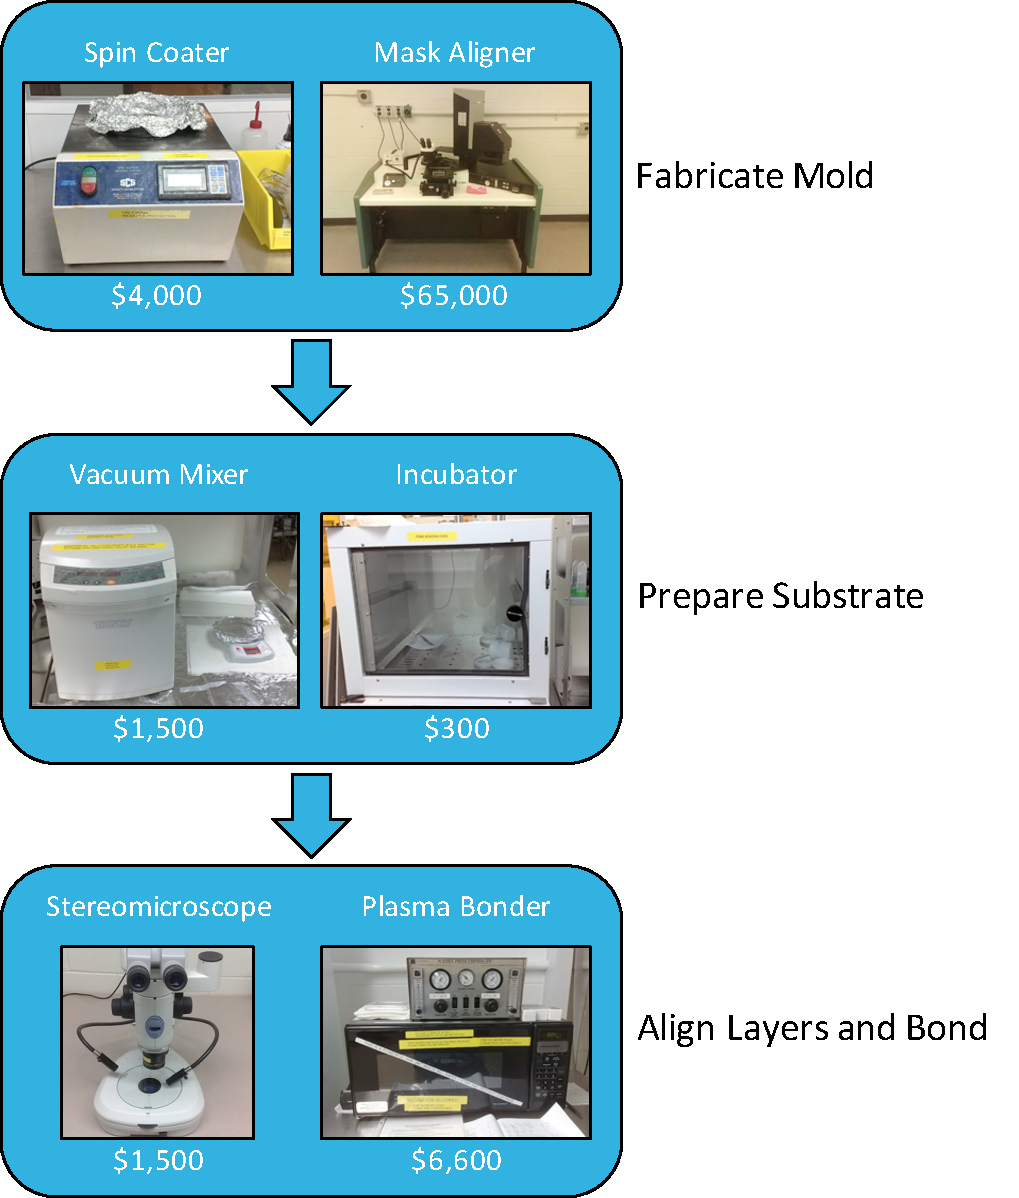
\includegraphics[width=6cm]{equipSoftLith.pdf}
    \medskip
  \end{minipage}\hfill
  \caption[Specialized equipment required to performform soft lithography]{Microfluidic fabrication via multi-layer soft lithography requires about \$80,000 in specialized equipment, not accounting for infrastructure, personnel, maintenance, or training. Cost estimates based on company quotes.}
    \label{fig:equipSoftLith}
\end{figure}


\subsection{Preparation of Substrate}
The substrate of choice for multi-layer soft lithography is a silicon elastomer known as polydimethylsiloxane (PDMS). This material is the result of combining a cross-linker and gel in a vacuum mixer, ensuring that no bubbles are present in the mixture. The flow layer is produced by carefully spin coating PDMS upon the silicon wafer ensuring that the features are fully immersed by the uncured elastomer. Excess elastomer is spun on top of the immersed features, which will result in the formation of a membrane used by the control layer to valve the flow of fluids. Unlike the flow layer, the control layer does not require the formation of a membrane of specified thickness, thus less precision is required for PDMS-coating the control layer's silicon mold. After coating, the PDMS for each layer is cured in an incubator.

\subsection{Alignment of Layers and Bonding}
After removing the PDMS from the silicon mold, the flow and control layers must be bonded together. This is often accomplished by modifying the surface chemistry of the PDMS using a plasma treatment. Each layer is placed, bonding-side-up in a plasma bonder. After removing the PDMS layers from the plasma bonder, the flow layer must be perfectly aligned with the control layer as the pneumatic valves must overlay their corresponding fluidic channels. This is accomplished by hand under a microscope and must be completed within a finite amount of time (often minutes) before the plasma treatment wears off. This process is then repeated to seal the fluidic layer to a piece of glass. 

\section{Programmability and the Microfluidic--Microelectronic Analogy}
\label{sec:backgroundCFRouting}

It is difficult to imagine a computer engineer having to create a VLSI layout and fabricate an ASIC every time they wanted to run a C program. While there will always be a place for custom circuit design in the world of digital electronics one basic tenant of digital design, namely abstraction, requires that it remain very much the exception rather than the rule. Unfortunately for the experimentalist, this is not the case in the field of microfluidics. The creation of custom, ``one-off'', designs for individual microfluidic experiments, no matter how user-friendly the corresponding CAD software is, could be is what is keeping the productivity of mLSI chips from achieving that of its silicon counterparts. Since Thorsen \emph{et al.} successfully integrated thousands of micromechanical valves in 2002 \cite{thorsen2002}, academic researchers have attempted to manage exponentially greater complexity in microfluidic design via the introduction of new design methodologies that attempt to introduce ``top-down'' specificity and move away from a ``bottom-up'' design philosophy \cite{minhass2013}\cite{melin2007}\cite{minhass2012} yet microfluidic experimentalists still find themselves in front of an oven baking a photoresist until it ceases to be sticky. 

Managing complexity is a necessary craft in that it allows the engineer to design complicated systems without becoming overwhelmed by details. The art of managing complexity in digital electronics design is  a mature process relative to that found in microfluidics. This is evident by the existence of larger scales of integration \emph{in silico} and by microfluidic efforts to create tools that mirror the design-to-execution workflow found in electronic computing. Examples of such tools are Micado, for automation of control layer routing \cite{amin2009}, Fluigi Place and Route \cite{fluigi}, and BioStream \cite{thies2008}. 

One goal of microfluidic technology is experimental automation. It could be argued that in order to achieve acceptable levels of automation then the expensive and time-consuming fabrication step should be removed from the work flow for the majority case as it is for electronic computation. Often, academic papers delving into the relm of mLSI begin by presenting an analogy between microfluidic LSI and LSI found in digital electronics. This research analogy seems strange as computer engineers can be productive using programmable tools (e.g., personal computers, Field Programmable Gate Arrays (FPGA), etc.) without having to know how to wash chemical from printed circuit boards (PCBs), use CAD tools to layout application specific integrated circuits (ASICs), or enlist the aid of experts in fabrication who can. Thus, the \emph{in silico} analogy does not hold when applied to the common-use case: that of the individual scientist or engineer, as the microfluidic experimentalist cannot adequately abstract away the details of device fabrication.

Abstraction works by placing the user at only the highest level relevant to the computation being performed and masking all underlying details. It can, therefore, be contended that functionally complete automation of microfluidic experiments carries the implication that experimentalists should be placed at only the highest levels of abstraction, thereby masking all underlying details. Currently, even the best efforts in microfluidic tools only remove intermediate levels of abstraction in device design (e.g., place and route), while exposing the scientist to the highest (e.g., device topology and function) \textbf{and lowest} (e.g., spin rate for optimal photoresist coverage) levels. Imagine if the only output of a C program were a circuit schematic that must first be built in order to obtain the result of the program. 

The use of the term ``working levels'' of complexity implies that the person operating within that layer need not concern themselves with the details of a lower layer, as such requirements would ultimately defeat the purpose of abstraction. Lower levels of detail are said to be ``abstracted'' away when their use is considered automatic. However, designers of systems residing in one particular abstraction layer should have an understanding of how their design decisions affect the layers immediately above and below the working layer, such as a C programmer understanding the nature of an address space \cite{Harris+Harris}. Theis \emph{et al} advocate for the creation of abstraction layers in microfluidics similar to that found in electronic computing \cite{thies2008}. These layers achieve success by focusing on three basic fluidic operations: mixing, transport and storage. Their BioStream protocol is a good first step in decoupling microfluidic architecture from biological computation by providing a common language for describing an experimental protocol. BioStream served initially as a standard language for reporting biological protocols but expanded to an end-to-end system that effectively describes biological protocols within the BioStream Fluidic ISA and executes them at the hardware level independent of microfluidic chip microarchitecture \cite{thies2008}. BioStream, however, does not fully address a functional purpose of abstraction, which is to provide automation, but it does accomplish a very important step the authors describe as a ``division of labor'' between the biology and microfluidic experts. 

There is, and probably always will be, a place in digital electronics for PCB design and ASIC fabrication. However, before an engineer decides to begin the process of building a custom PCB or layout a new ASIC they should first consider how their deisgn decision addresses the productivity gap. In order to proceed, a working definition of the term ``productivity'' must be presented. Process and requirements engineers \cite{Review_ProcessEngr} have defined productivity strictly in terms of hours saved \cite{CostBenefit_hours}, as a function of on-time delivery \cite{OnTimeDelivery} or as some measure of quality \cite{Quality}. This paper will define the productivity of a particular method as the number of hours saved through the implementation of a particular process.

Device fabrication is not a task oft performed by a computer scientist. Rather, a computer scientist spends many hours debugging a program such that it runs reliably and correctly within the confines of a particular ISA. This exemplifies the nature of design discipline. It is well-within the realm of possibility for a computer engineer to give up debugging a program and reach for a CAD tool, with which to build a custom chip designed for their particular purposes. That scenario would only make sense if the final custom-fabricated solution could overcome the extremely large gap in productivity inherent to designing and fabricating it. The amount of lead-time required to design and build an ASIC or PCB could significantly outweigh the benefits of having a single custom-chip to use only in very specific circumstances and only within that one engineer's lab. Why then is this practice deemed acceptable in microfluidics?

Even attempts to create some framework for flow-based microfluidic design, such as a common microfluidic ISA\cite{amin2009} or predefined software modules \cite{soe2013} are still, fundamentally, design methods requiring chip fabrication. Microfluidic chip fabrication is a highly unproductive in that it requires many hours to design and build a device incapable of performing diverse and repeatable experiments. Fortunately for the computer engineer there exists other prototyping options besides PCBs and ASICs, such as the use of a field programmable gate array (FPGA) or a microcontroller. The microfluidic experimentalist is left with only one prototyping option that almost always requires some level of device
fabrication.

Chapter \ref{chapter:xposer} outlines a novel primitive for continuous-flow microfluidics aimed at unlocking elements of programmability in continuous-flow devices. It analyzes and solves microfluidic design challenges using tools for automated design and control, ultimately providing a solution that would allow the microfluidic experimentalist to be one step closer to realizing the productivity potential of true large-scale integration. 


\section{Pathogen Identification and Antibiotic Susceptibility Testing}
\label{sec:cellSep}

The World Health Organization listed infectious disease as the second leading cause of death worldwide \cite{world2004world}. One explanation as to why infections are particularly deadly is that multiple days of lab processing are currently required to determine a particular bacterial identity and its antibiotic susceptibility profile. In the interim, infections are often treated using broad-spectrum antibiotics, which has resulted in the rise of antibiotic resistance and diminished clinical efficacy \cite{laxminarayan2013antibiotic}. The ultimate goal of the IDAST program at the Charles Stark Draper Laboratory is to determine information regarding a pathogen's phenotype and antibiotic susceptibility at the point of care within the time-frame of a single visit to the doctor. This is performed using a multi-staged approach shown in Figure \ref{fig:idastFlow}, whereby a microfluidic system purifies a bacterial sample from whole blood in preparation for a downstream biological assay resulting in an optical readout.

\begin{figure}[h]
  \begin{minipage}[t]{0.99\linewidth}\centering
    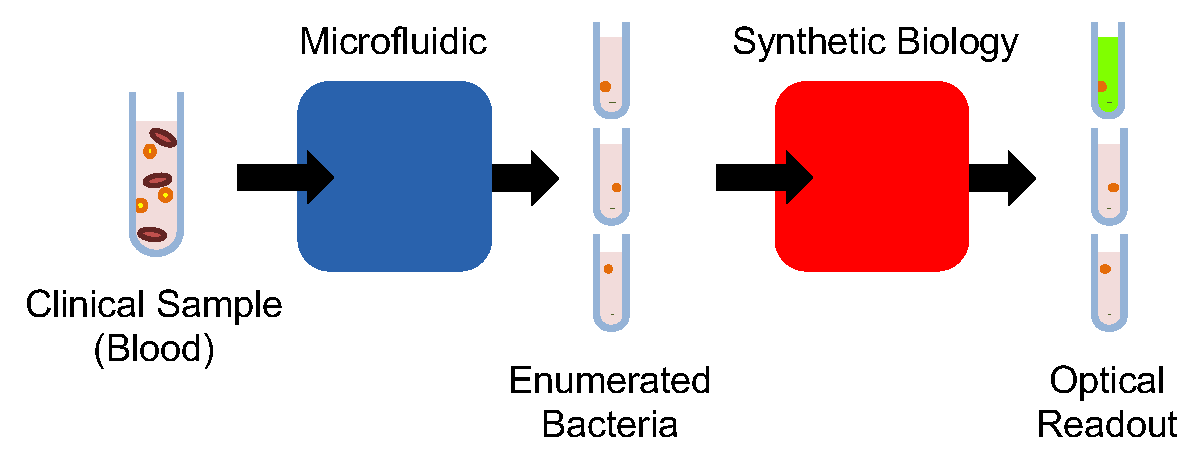
\includegraphics[width=13cm]{idastFlow.pdf}
    \medskip
  \end{minipage}\hfill
  \caption[System-level view of IDAST]{IDAST is performed using a microfluidic device for sample processing followed by a proprietary synthetic-biological approach resulting in an optical readout.}
    \label{fig:idastFlow}
\end{figure}

The microfluidic system is comprised of the three stages shown in Figure \ref{fig:idastUfFlow}. The separation step is responsible for removing the large blood components, such as red blood cells (RBCs) and white blood cells (WBCs) from a diluted whole-blood sample. It then uses a trapping stage to concentrate the bacterial sample and wash away smaller blood components (e.g., plasma, platelets, etc.). Finally, clean bacterial samples are enumerated and distributed into multiple wells for downstream processing using synthetic biology. The microfluidic leverages acoustic manipulation to accomplish the first two stages, the first of which is the subsystem MakerFluidics sought to optimize. Acoustic manipulation is described in further detail in Section \ref{sec:acoust_intro}.

\begin{figure}[h]
  \begin{minipage}[t]{0.99\linewidth}\centering
    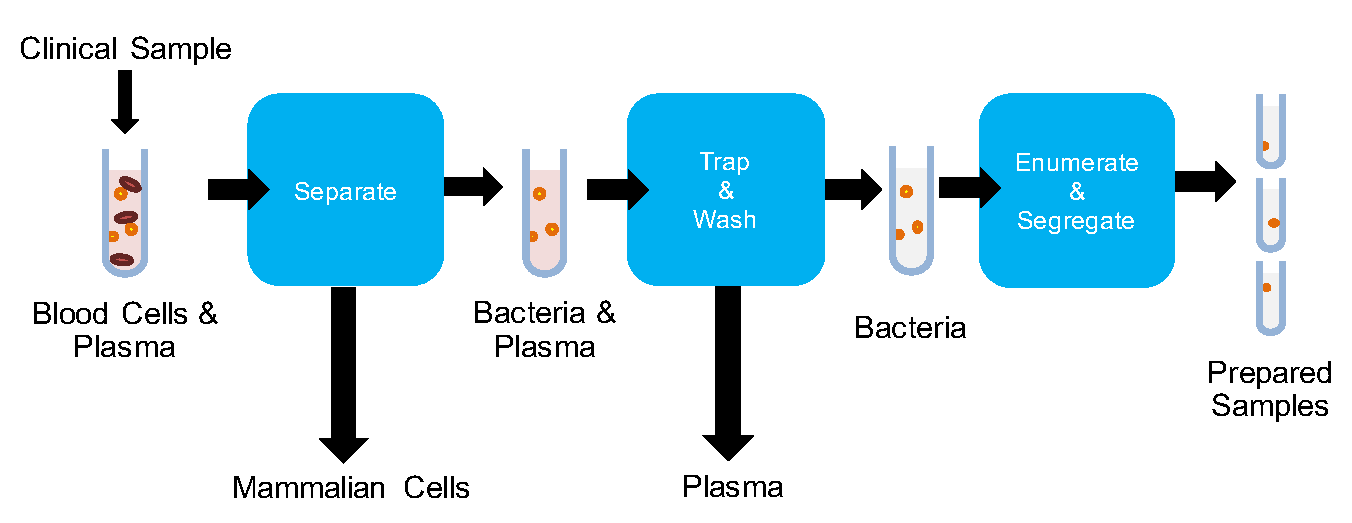
\includegraphics[width=13cm]{idastUfFlow.pdf}
    \medskip
  \end{minipage}\hfill
  \caption[Block diagram of IDAST sample processing via microfluidics]{Sample processing for IDAST can occur in a microfluidic composed of three stages: separation, trap and wash, and enumerate and segregate. MakerFluidics was responsible for optimizing the first subsystem, namely separation.}
    \label{fig:idastUfFlow}
\end{figure}

\cleardoublepage



% -------------------------------------
% CHAPTER 2: MakerFluidics
% -------------------------------------
\chapter{The MakerFluidics Framework}
\label{chapter:mf}
\thispagestyle{myheadings}

% set this to the location of the figures for this chapter. it may
% also want to be ../Figures/2_Body/ or something. make sure that
% it has a trailing directory separator (i.e., '/')!
\graphicspath{{2_MakerFluidics/Figures/}}

\section{Introduction}
\label{sec:mfIntro}

MakerFluidics is a microfluidic fabrication and control framework that operates within a set of constraints guided by the ideals of automation and the modern ``maker movement''. This framework integrates into the larger microfluidic design flow shown in Figure \ref{fig:fullflow}, but it can also be employed on its own. MakerFluidics accepts physical and temporal valve control requirements and a microfluidic device design as inputs and provides the necessary control software, manufacturing files and assembly information required to build a self-contained microfluidic device and control infrastructure.

\section{Problem Statement}
\label{sec:mfPS}
A significant aim of the modern maker movement is to make technology and technological ``know-how'' accessible to the masses. One way to accomplish this goal is to devise solutions using resources that are flexible and ubiquitous \cite{schrock2014education}. A significant criticism often levied against the field of microfluidics is its high barrier to entry often as a result of the need for highly specialized fabrication and control equipment as well as expertise that is typically found only in labs dedicated to microfabrication \cite{whitesides2006}. This work seeks to create a design-to-device, automated microfluidic work-flow constrained by the ideals espoused in maker culture. 

\begin{figure}[h]
  \begin{minipage}[t]{0.99\linewidth}\centering
    \includegraphics[width=14cm]{fullflow.pdf}
    \medskip
  \end{minipage}\hfill
  \caption[Microfluidic specify--design--build workflow]{MakerFluidics is part of a larger microfluidic design flow that spans from biological specification to microfluidic fabrication and control}
    \label{fig:fullflow}
\end{figure}


\section{Contstraints}
\label{sec:mfConstraints}
An important goal of the maker movement is to increase technology's accessibility. This ideal is levied on MakerFluidics in the form of a series of constraints, the first of which is that all fabrication equipment must be sourced through ubiquitous consumer and retail product outlets such as Amazon.com in the Unites States, or Amazon.ca, .co.uk, .jp, etc. internationally, and each individual piece of equipment required for fabrication and control must cost less than \$100. A desktop computer numerical control (CNC) mill and 3D printer are excepted from this constraint on the basis that they are common maker-space tools with a wide variety of uses extending well beyond the field of microfluidics; the cost of the CNC mill (Othermill, Othermachine Co.) and 3D printer (Ultimaker 2, Ultimaker B.V.) used in our lab are each less than \$2,500. Additionally, all elements of the complete software tool chain must be free and/or open-source. 

To further facilitate microfluidic accessibility, all fabrication and control protocols must be accomplished without specialized infrastructure beyond a wall electrical outlet. This excludes fume hoods, clean room facilities, tank storage, vacuum lines and corona/plasma bonders. The process for designing, fabricating and controlling programmable (i.e., valved) microfluidics within the specified constraints is explored. Each stage of the process includes a comparison of current methods to methods developed or adopted by the MakerFluidics framework. 

\begin{table}[H]
% table caption is above the table
\caption[Infrastructure requirements for soft lithography versus MakerFluidics]{Necessary infrastructure to perform soft lithography versus that required for MakerFluidics.}
\label{tab:mfInf}       % Give a unique label
% For LaTeX tables use
\centering
\begin{tabular}{lcc}
\hline\noalign{\smallskip}
Infrastructure & MakerFluidics & Soft Lithography\\
\noalign{\smallskip}\hline\noalign{\smallskip}
Clean Room & Not Required & Required \\
Fume Hood & Not Required & Required \\
Vacuum Line & Not Required & Required \\
Tank Storage & Not Required & Required \\
Electrical Outlet & Required & Required \\
Equipment Overhead & ~\$4,000 & ~\$80,000 \\
\noalign{\smallskip}\hline
\end{tabular}
\end{table}


\section{Microfluidic Design}
\label{sec:mfDesign}

Three levels of software are required to design and fabricate a novel chip geometry using a CNC micromill: a computer aided design (CAD) tool is used to create a solid model of the device; computer aided manufacturing (CAM) software generates the commands (also called toolpaths) that are sent directly to the micromill; and control software manages the connection between a computer and the micromill and sends individual toolpaths to the micromill. 

Device designs were created using OpenSCAD \cite{wikiOpenScad}, a free and open source CAD tool that reads script files to generate solid models. The ability to describe a solid model using only text is an important distinction between OpenSCAD and typical 3D modeling software packages (ex., AutoCAD, SolidWorks, etc.), which often require geometries to be manually drawn. Text-based modeling allows for automatic generation of device designs using a CAD workflow, such as that shown in Figure \ref{fig:fullflow}. MakerFluidics leverages OpenSCAD by creating device primitives that are stored in custom libraries. As shown in Listing \ref{lst:XposerChip}, these primitives are parametric, allowing them to be ``called'' in a fashion similar to that of an object-based programming language. 

\begin{minipage}{0.95\linewidth}
\centering 
	\begin{lstlisting}[caption={This single line of OpenSCAD creates the 3D model shown in Figure \ref{fig:mfParams}(A). Once a primitive is defined in OpenSCAD, the parameters associated with each device geometry can be modified and the corresponding solid model will adjust to reflect the changes.},label={lst:XposerChip}, frame=single, language=scad]
  transposerNet(N=3, w_channel=1, r_valve=1, scale_x = 1);
\end{lstlisting}
\end{minipage}

Once a solid model is created using a CAD tool, the solid model must be imported by CAM software in order to generate the toolpaths that will be sent to the mill. MakerFluidics uses Autodesk Fusion 360 to create toolpaths for 3D models, such as mesh models (ex., an STL file). All three CNC mills tested in the lab (Othermill V2 by Othermachine Co.; Othermill Pro by Othermachine Co.; and Nomad 883 by Carbide 3D) have machine-specific control software with the capability to directly process 2D models, such as a vector-graphics file (ex., an SVG file). All of the CAM software listed above is free, but not necessarily open source. A standard operating procedure for interacting with Fusion 360 in order to generate toolpaths and operate the Othermill V2 or the Othermill Pro can be found in Appendix \ref{appendix}.


\begin{figure}[h]
  \begin{minipage}[t]{0.99\linewidth}\centering
    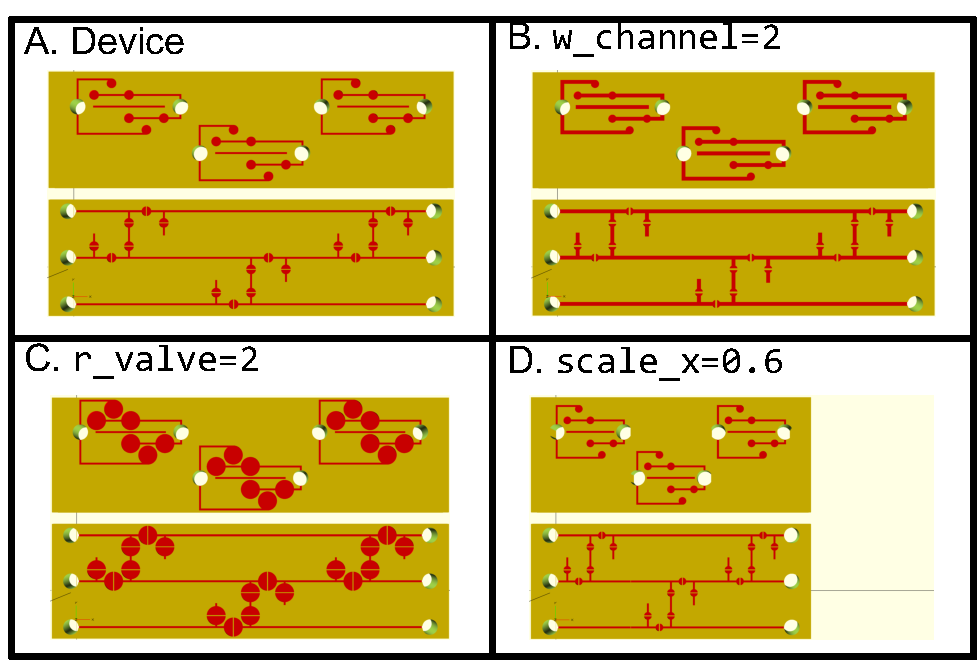
\includegraphics[width=14cm]{params.pdf}
    \medskip
  \end{minipage}\hfill
  \caption[Example device parameters]{Example parameters associated with a network of transposer primitives. The primitive and routing topology are presented in detail in Chapter \ref{chapter:xposer}. (A) shows the baseline device. (B) illustrates modifying the channel parameter to make the channels wider. (C) shows how the valve dimensions can be modified using a parameter associated with valve radius. (D) shows how the entire device can scale in the x-dimension using yet another parameter.}
    \label{fig:mfParams}
\end{figure}

\section{Microfluidic Fabrication}
\label{sec:mfFabrication}
The fabrication of a microfluidic device typically has two main steps: pattern geometries and seal layers \cite{mcdonald2002poly}.

\subsection{Pattern Geometries}
Channel and valve geometries are etched in thermoplastic polymers using a desktop CNC mill. This stands in sharp contrast from conventional methods of microfluidic fabrication, namely photolithography and wet etching, which require the use of clean room facilities and highly specialized equipment. The CNC approach is well-suited for integrating valving technologies such as monolithic membrane valves \cite{grover2003monolithic} (Figure \ref{fig:valves}) and centrifugal capillary valves \cite{madou1998labcd}. A significant trade-off for the relative ease of CNC milling thermoplastics using a desktop (i.e., not industrial-grade) CNC mill is that the maximum resolution is ~25$\mu$m with an exponential increase in reliability seen at feature sizes greater than 250$\mu$m \cite{guckenberger2015micromilling}, whereas microfluidic geometries using conventional methods such as photolithography can reliably achieve features smaller than 1$\mu$m \cite{mcdonald2002poly}.

\begin{figure}[h]
  \begin{minipage}[t]{0.99\linewidth}\centering
    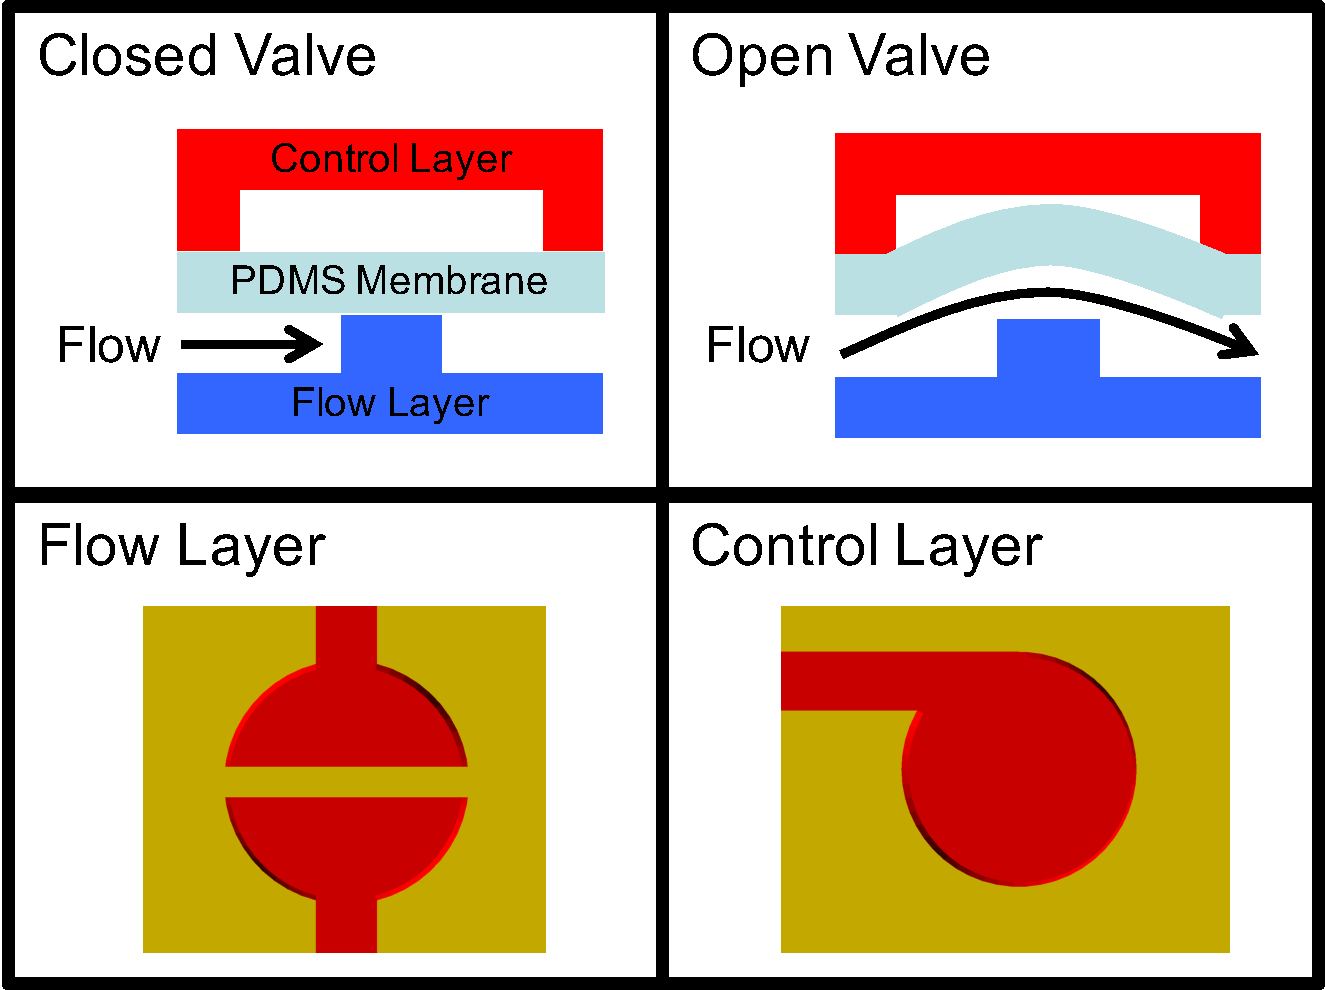
\includegraphics[width=14cm]{valves1.pdf}
    \medskip
  \end{minipage}\hfill
  \caption[Illustration of valving primitive]{Normally-closed monolithic membrane valves \cite{grover2003monolithic} are realized by introducing discontinuities in the flow layer (blue) and a corresponding pneumatic cavity in the control layer (red). These two layers are separated by a PDMS membrane. To open the valve a vacuum is introduced into the cavity in the control layer.}
    \label{fig:valves}
\end{figure}

\begin{table}[H]
% table caption is above the table
\caption[Dimensional constraints of soft lithography versus MakerFluidics]{Published dimensional constraints regarding devices fabricated using the MakerFluidics protocol versus that of soft lithography. Aspect Ratio is defined as feature height to feature width.}
\label{tab:mfDims}       % Give a unique label
% For LaTeX tables use
\centering
\begin{tabular}{p{2cm}ccp{4cm}}
\hline\noalign{\smallskip}
Dimension & MakerFluidics & Soft Lithography & Reference \\
\noalign{\smallskip}\hline\noalign{\smallskip}
\multirow{2}{*}{Aspect Ratio} & Tool Dependant & \multirow{2}{*}{1:20} & \cite{schaller1999microstructure}\\ 
& (often 3:1) & & \cite{qin2010soft}{\smallskip}\\
  \hline\noalign{\smallskip}
Minimum & Tool Dependant & \multirow{3}{*}{$<$1$\mu$m} & \cite{sweatt2008diamond}\\ 
Feature & (25$\mu$m Demonstrated) & & \cite{qin2010soft}\\
Size & (5$\mu$m Theoretical) & & {\smallskip}\\
  \hline\noalign{\smallskip}
  Minimum & \multirow {3}{*}{25$\mu$m} & \multirow{3}{*}{$<$1$\mu$m} & \cite{yen2016cost}\\ 
Feature & & & \cite{qin2010soft}\\
Spacing & & & {\smallskip}\\
  \hline\noalign{\smallskip}
  Bonding Capacity & \multirow{2}{*}{5 psi} & \multirow{2}{*}{50 psi} & \cite{mcdonald2002poly}{\smallskip}\\
  \hline\noalign{\smallskip}
\multirow{3}{*}{Materials} & Thermoplastics & PDMS & \cite{schaller1999microstructure}\\
& Soft Metals & Silicon & \cite{qin2010soft}\\
& Cured Thermosets & & \\
\noalign{\smallskip}\hline
\end{tabular}
\end{table}


\subsection{Seal Layers}
Once geometries are etched into the desired substrate, sealing these channels becomes the next challenge. Polydimethylsiloxane (PDMS) is a common material for fabricating microfluidics \cite{mcdonald2002poly} and is also commonly used to encapsulate solar panels and outdoor lighting. It is because of the latter property that PDMS (Sylgard 184, Dow Corning) is available through retail outlets, such as Amazon, and, thus, falls within the constraints for adoption by the MakerFluidics fabrication paradigm. PDMS can be sealed irreversibly through modifications to its surface chemistry via plasma or corona exposure or sealed reversibly simply using the material's inherent Van der Waals attraction to various materials including itself, glass and thermoplastics \cite{mcdonald2002poly}. Since irreversible sealing through surface treatments involves specialized machinery, MakerFluidics employs the latter method via Van der Waals force. The trade-off being that the reversible seal cannot withstand pressures greater than 5psi \cite{mcdonald2002poly}. The entire protocol is summarized in Figure \ref{fig:fabFlow}.


\begin{figure}[h]
  \begin{minipage}[t]{0.99\linewidth}\centering
    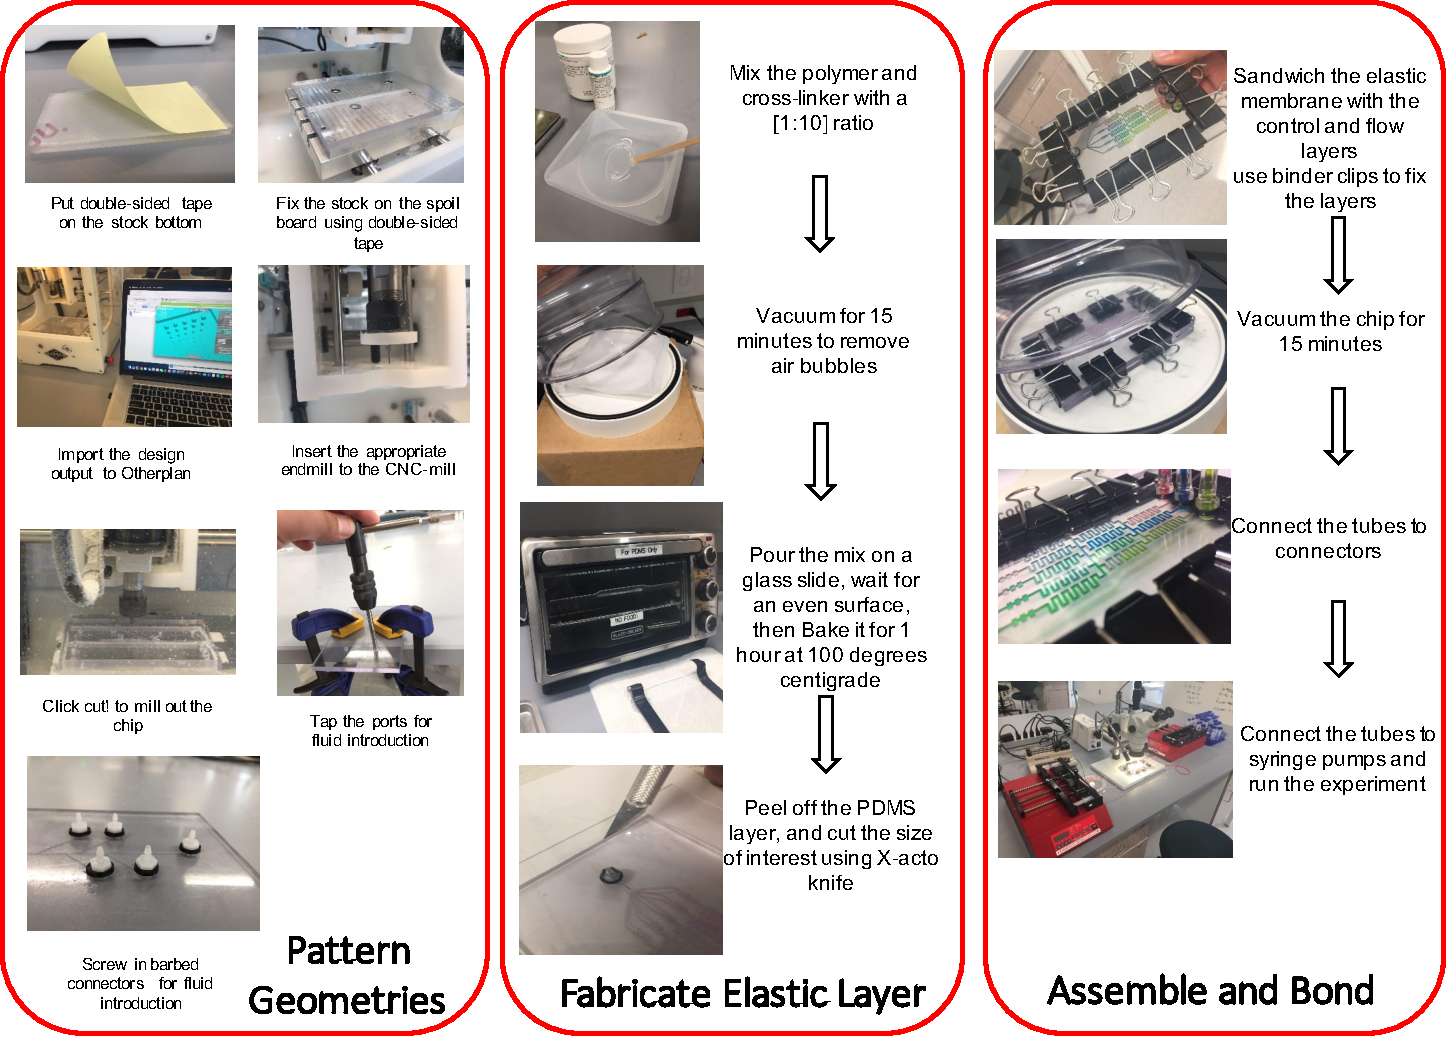
\includegraphics[width=14cm]{fabFlow.pdf}
    \medskip
  \end{minipage}\hfill
  \caption[The MakerFluidics fabrication protocol]{Workflow for fabricating microfluidics using the MakerFluidics framework.}
    \label{fig:fabFlow}
\end{figure}




\section{Experimental Control}
\label{sec:mfControl}
MakerFluidics views experimental conditions as a sequence of temporally-specified valve conditions. This necessitates a data structure consisting of an enumerated array of valve objects and a sequence of temporal specifications regarding their state. This data structure can be automatically generated by microfluidic CAD software developed in house, but it can also be created manually as a series of wait statements and valve conditions shown in Figure \ref{fig:sequence}. These valve objects are linked to the microfluidic layout provided to the fabrication software through the use of a graphical user interface (GUI).

Pneumatics are provided through an array of 3D printed syringe pumps controlled by custom firmware on an Arduino microcontroller. This microcontroller receives serial commands derived from the GUI running on a host computer. The MakerFluidics control GUI and firmware is extensible and interoperable with a conventional, solenoid-driven control infrastructure.

\begin{figure}[h]
  \begin{minipage}[t]{0.99\linewidth}\centering
    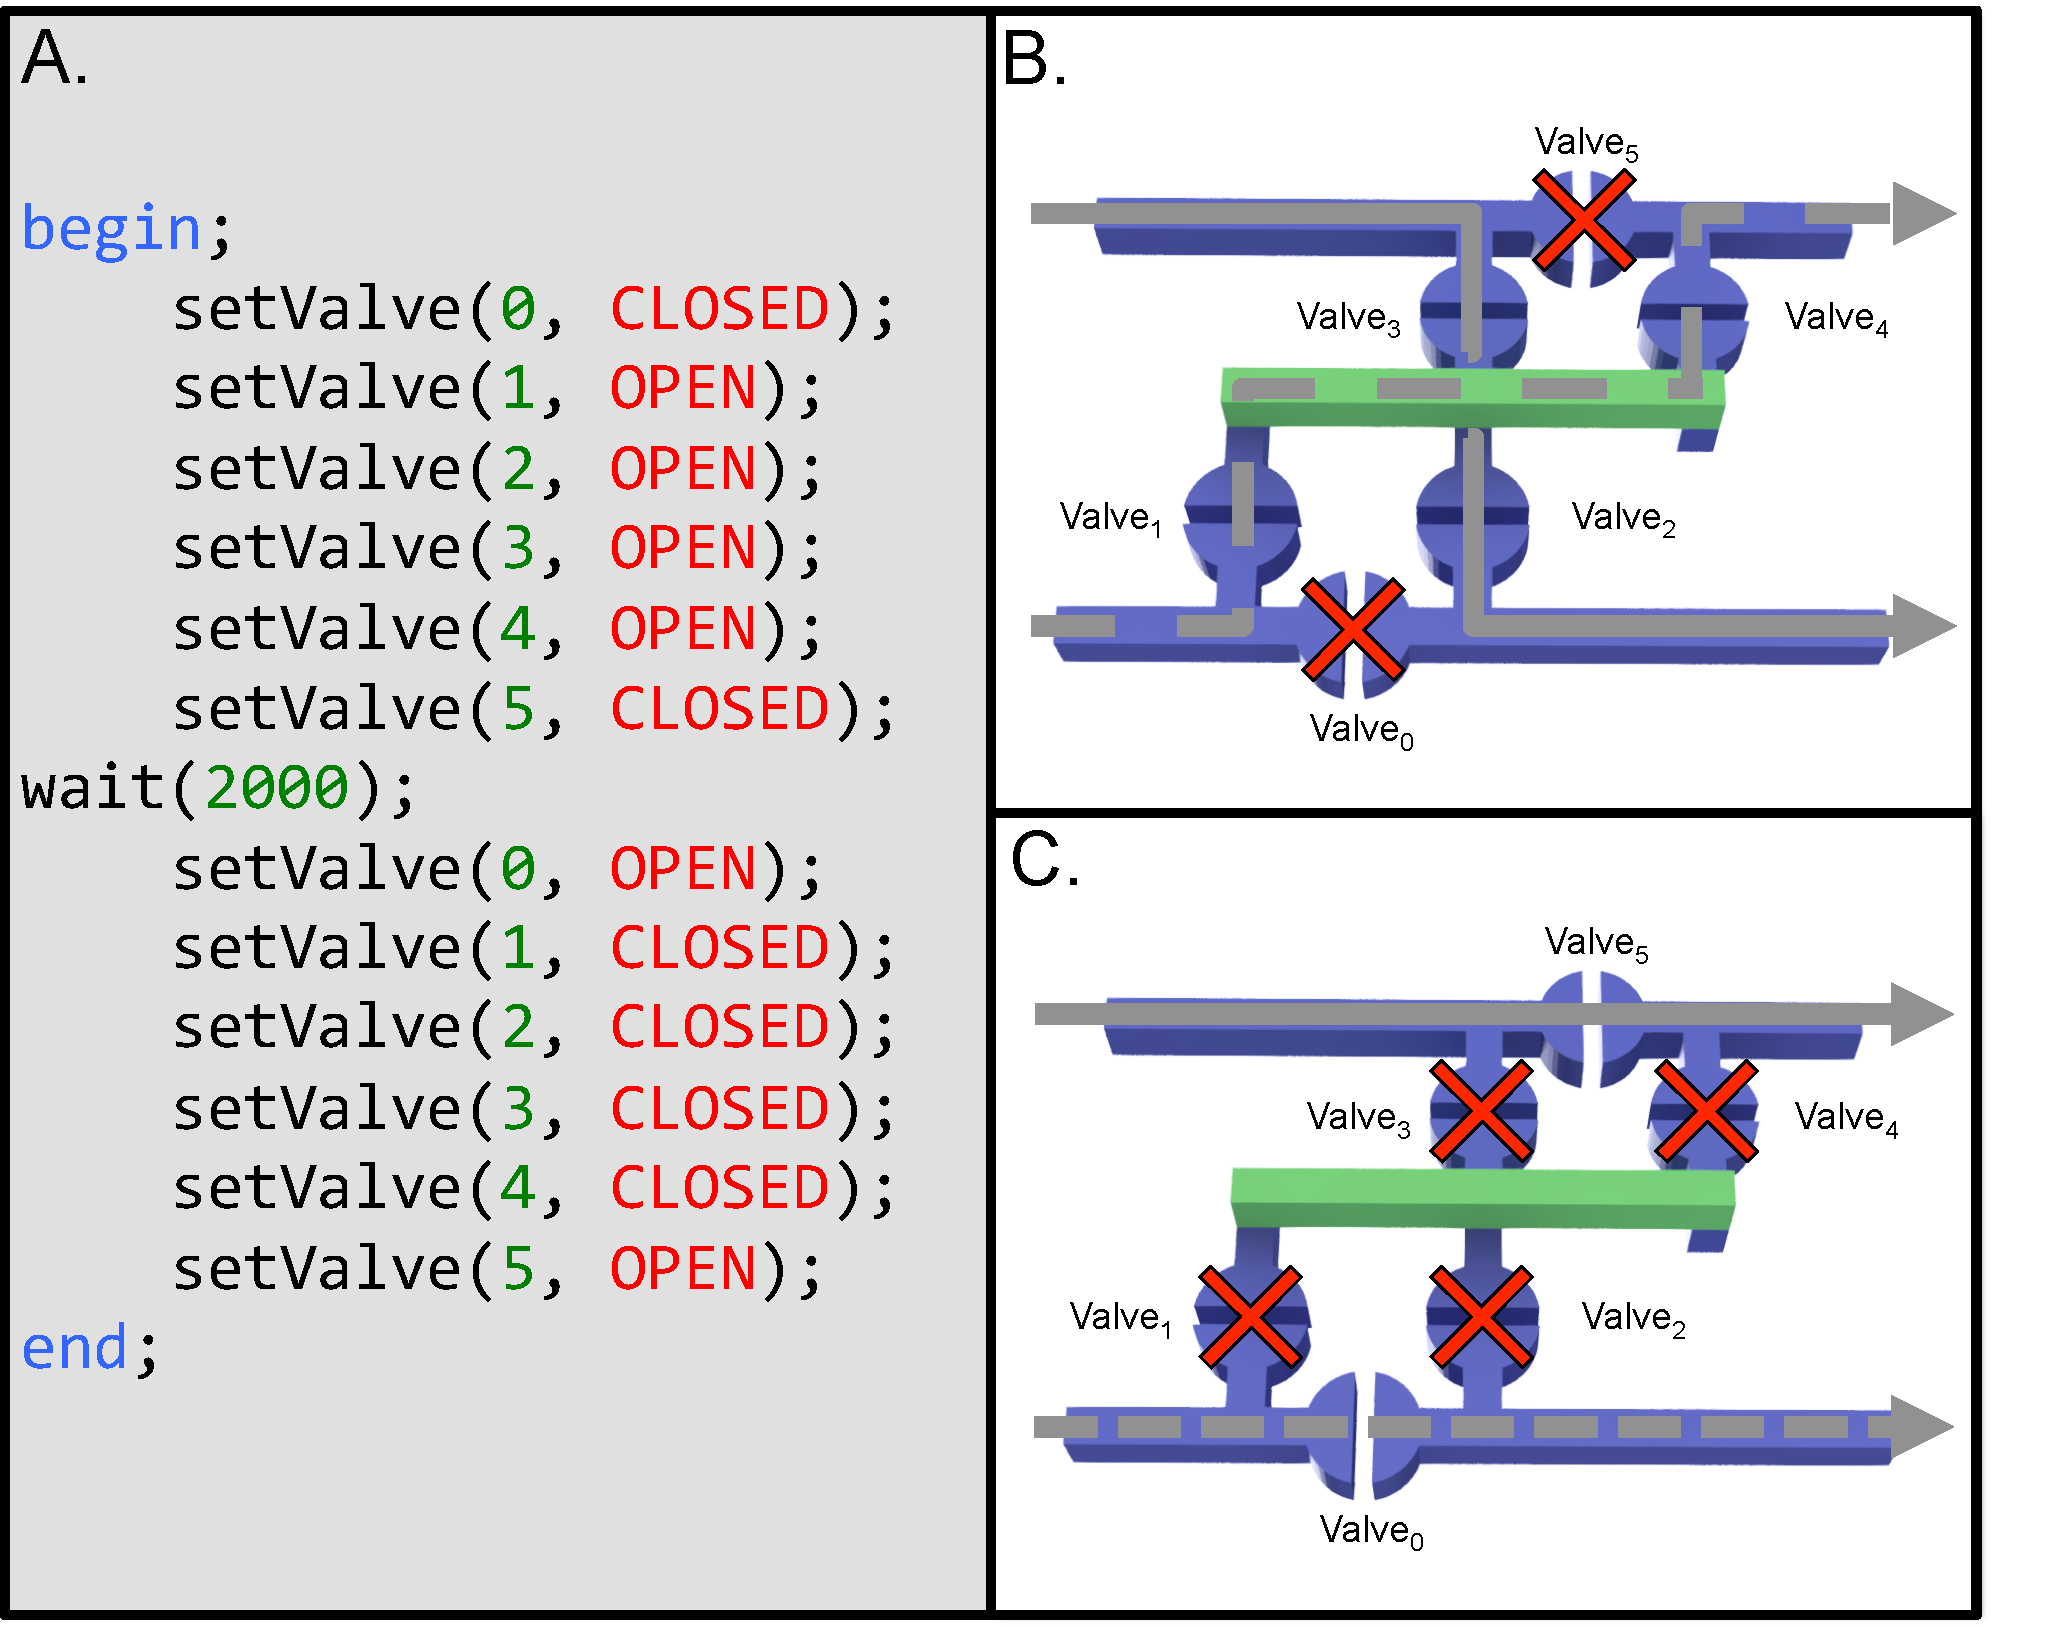
\includegraphics[width=14cm]{sequence.pdf}
    \medskip
  \end{minipage}\hfill
  \caption[Valving sequence temporal specification]{The temporal specification (A) \cite{thies2008} for a device containing six valves (B, C). The specification in (A) dictates the set of conditions in (B) to begin the assay. After 2000ms the valves change state to that shown in (C), thus affecting the movement of fluid through the device.}
    \label{fig:sequence}
\end{figure}

\section{Applicability of MakerFluidics}
\label{sec:mfApplicability}
While the collection of protocols and technologies that define MakerFluidics may seem simplistic, the relevance of the framework was demonstrated by  its ability to design, fabricate, and control a complex network of novel microfluidic primitives, as described in the subsequent chapter. Additionally the framework was used to fabricate experimentally relevant devices in industry. This work is presented in Chapter \ref{chapter:acoust}.

\cleardoublepage

% -------------------------------------
% CHAPTER 3: Transposer
% -------------------------------------
\chapter{A reconfigurable continuous-flow fluidic routing fabric using a modular, scalable primitive}
\label{chapter:xposer}
\thispagestyle{myheadings}

% set this to the location of the figures for this chapter. it may
% also want to be ../Figures/2_Body/ or something. make sure that
% it has a trailing directory separator (i.e., '/')!
\graphicspath{{3_xposer/Figures/}}

\section{Introduction}
\label{sec:xposer_intro}
Microfluidic devices, by definition, are required to move liquids from one physical location to another. Given a finite and frequently fixed set of physical channels to route fluids, a primitive design element that allows reconfigurable routing of that fluid from any of  \textit{n} input ports to any \textit{n} output ports will dramatically change the paradigms by which these chips are designed and applied. Furthermore, if these elements are ``regular'' regarding their design, the programming and fabrication of these elements becomes scalable. This paper presents such a design element called a \textit{transposer}. We illustrate the design, fabrication and operation of a single transposer. We then scale this design to create a programmable fabric towards a general-purpose, reconfigurable microfluidic platform analogous to the Field Programmable Gate Array (FPGA) found in digital electronics.

\section{Problem Statement}
\label{sec:xposer_ps}
Engineering frequently involves the exploration of design tradeoffs. Such tradeoffs include time versus quality or performance versus cost \cite{otto1991trade}. A tradeoff frequently encountered in the design of microfluidic systems is specificity versus flexibility. Devices that perform specific tasks often can do these tasks with great precision and quality but users require new devices and/or device architectures for each subsequent task \cite{fidalgo2011}. This lack of re-use increases the cost of experimentation over time, requires re-training for each device, and prevents common platforms for legitimate comparison of results across experiments. Flexible devices on the other hand may not meet stringent performance requirements or the cost of reconfiguring devices may be prohibitively high in terms of time or training \cite{thies2008}. A microfludic device that offers both the performance of a specific solution with the programmability of a flexible solution coupled with low financial as well as time costs would enable entirely new classes of experimentation and design.

Continuous-flow microfluidic chip architectures have yet to fully benefit from the reconfigurable flexibility offered by digital microfluidics \cite{fair2007digital}. Digital microfluidics benefit from extensive research on routing algorithms \cite{curtis2015simulation} that avoid cross-contamination stemming from undesired droplet collisions \cite{cho2008droplet}. These algorithms are predicated on the classification of fluids as discrete droplets, rather than as a continuous-flow. Additionally, digital microfluidic routing algorithms presume that droplets are able to bypass others using a grid of prefabricated paths, combined with the ability to stop the movement of some droplets while continuing to position others \cite{zhao2012droplet}. In contrast, continuous-flow microfluidics must maintain continuous-flow for correct operation of devices such as gradient generators \cite{hung2005continuous}, cell traps \cite{el2006cells}, and batch separators \cite{pamme2007continuous}, thus interrupting flow for the purposes of fluid routing is undesirable. This distinguishes the fluid routing problem from that of a digital microfluidic chip, but it also makes the problem analogous to signal routing in electronic digital design where wires cannot both carry a signal and intersect, which could result in a metastable condition \cite{kleeman1987metastable}.

One approach to the challenge of continuous-flow routing is to examine how reconfigurable computing hardware \cite{todman2005reconfigurable} provides both highly specific, yet programmable, computing elements linked together using a flexible routing fabric \cite{compton2002reconfigurable}. Such an approach retains the specificity of the dedicated resources while allowing those resource relationships (e.g. input and output) to be defined dynamically. Lessons gleaned from the development of modern reconfigurable platforms in the digital electronics domain, namely island-style FPGAs \cite{schmit2005extra}, tell of the need for two major architectural components \cite{kuon2008}:
\begin{enumerate}
	\item Functional primitives that scale regularly, lending to automated design placement
	\item A routing architecture that actuates regularly, lending to automated, dynamic signal routing
\end{enumerate}

These architectural components must then be linked to a control environment using software that scales with the architecture. This requirement prevents chip designers from having to generate artisanal control software for every new chip architecture. As this work demonstrates, the regularity of the primitive and routing structure is what allows for algorithmic scaling in design and control. 

Examples of functional, continuous-flow microfluidic primitives that scale regularly are multiplexors \cite{thorsen2002}, storage elements \cite{thies2008}, culture chambers \cite{fidalgo2011} and mixers \cite{jensen2013}. Chip designs using scalable microfluidic primitives in the absence of a dynamic routing architecture carry similar tradeoffs to those found while designing electronic Application Specific Integrated Circuits (ASICs), whereby the major constraint is that, once implemented, these functional primitives are effectually ``frozen in silicon,'' or in the case of many microfluidic chips: ``frozen in polydimethylsiloxane (PDMS).'' 

\section{Related Work}
\label{sec:xposer_rw}
Microfludics at chip densities belonging to the classes of large scale integration (LSI), i.e., chips with hundreds to thousands of components \cite{thorsen2002}, and very large scale integration (vLSI), i.e., millions of components, have been demonstrated \cite{araci2014}. Electronic Design Automation (EDA) tools for automated design \cite{mcdaniel2013}, layout \cite{huang2014}, and control \cite{thies2008} of these types of chips have also been developed. However, each tool and design paradigm cited above views signal routing as a static problem akin to signal routing in electronic ASIC design, the primary constraint being that continuous-flow channels cannot both carry a signal and intersect on the same fluidic layer without being separated by a valve. EDA tools and chip architectures can overcome this constraint by either incorporating design rules that necessitate the avoidance of channel collisions \cite{huang2014} or dealing with channel collisions individually through the creation of new primitives such as underpasses and vias \cite{huft2013microfluidic}. Additionally, some attempts at channel routing incorporate an element of programmability that necessitates interruption in continuous flow to achieve arbitrary routing \cite{thorsen2002}. These programmable architectures will be be described in further detail in Section \ref{ssec:alts}. What these efforts lack is an ability, integrated into both the chip architecture and control environment, to dynamically route signals to any functional primitive post-fabrication while maintaining continuous-flow and, thus, create a general-purpose fluidic architecture. Only by unlocking this capability can the field of continuous-flow microfluidics expand its design spectrum to include general-purpose platforms among its vast repertoire of application-specific chips thus mirroring the evolution of digital electronics towards experimental pervasiveness. 

This work addresses that need, namely for a scalable, continuous-flow fluidic routing architecture using a network of pre-fabricated channels and integrated software for automated device actuation. A key contribution is the introduction of a ``transposer'' primitive. Transposers allow for a reconfigurable routing fabric. This architecture allows microfluidic chips incorporating high chip densities to better realize the benefits of scaling and come closer to achieving the functional ubiquity of digital electronics.

\section{Primitive Architecture}
\label{sec:primArch}
The theory of operation for a single transposer primitive is shown in Figure \ref{fig:op}. Valves were designed using a monolithic membrane technique previously described \cite{grover2003monolithic}. Briefly, normally closed valving mechanisms are created by introducing discontinuities in a flow channel. These discontinuities are covered by the elastomeric membrane. A corresponding pneumatic cavity is patterned on the control layer \cite{grover2006development}. When a vacuum is introduced into the pneumatic cavity, the elastomer is distended into the cavity, thus allowing flow to proceed in the channel \cite{nguyen2012}. 

A transposer primitive has the ability to selectively swap the contents of two channels, allowing the user to route fluids through the chip dynamically while maintaining continuous-flow. This design requires that one channel ``jump'' over another by traversing between the flow and control layers. One transposer primitive will have two input ports and two output ports. As shown in Figure \ref{fig:modes}, the primitive can take on one of two modes: crossed or straight. In the straight mode, fluids will pass through the primitive unbroken. When the primitive is crossed the contents of both inputs are swapped when viewed from the output ports. 
\begin{figure}[h]
  \begin{minipage}[t]{0.99\linewidth}\centering
    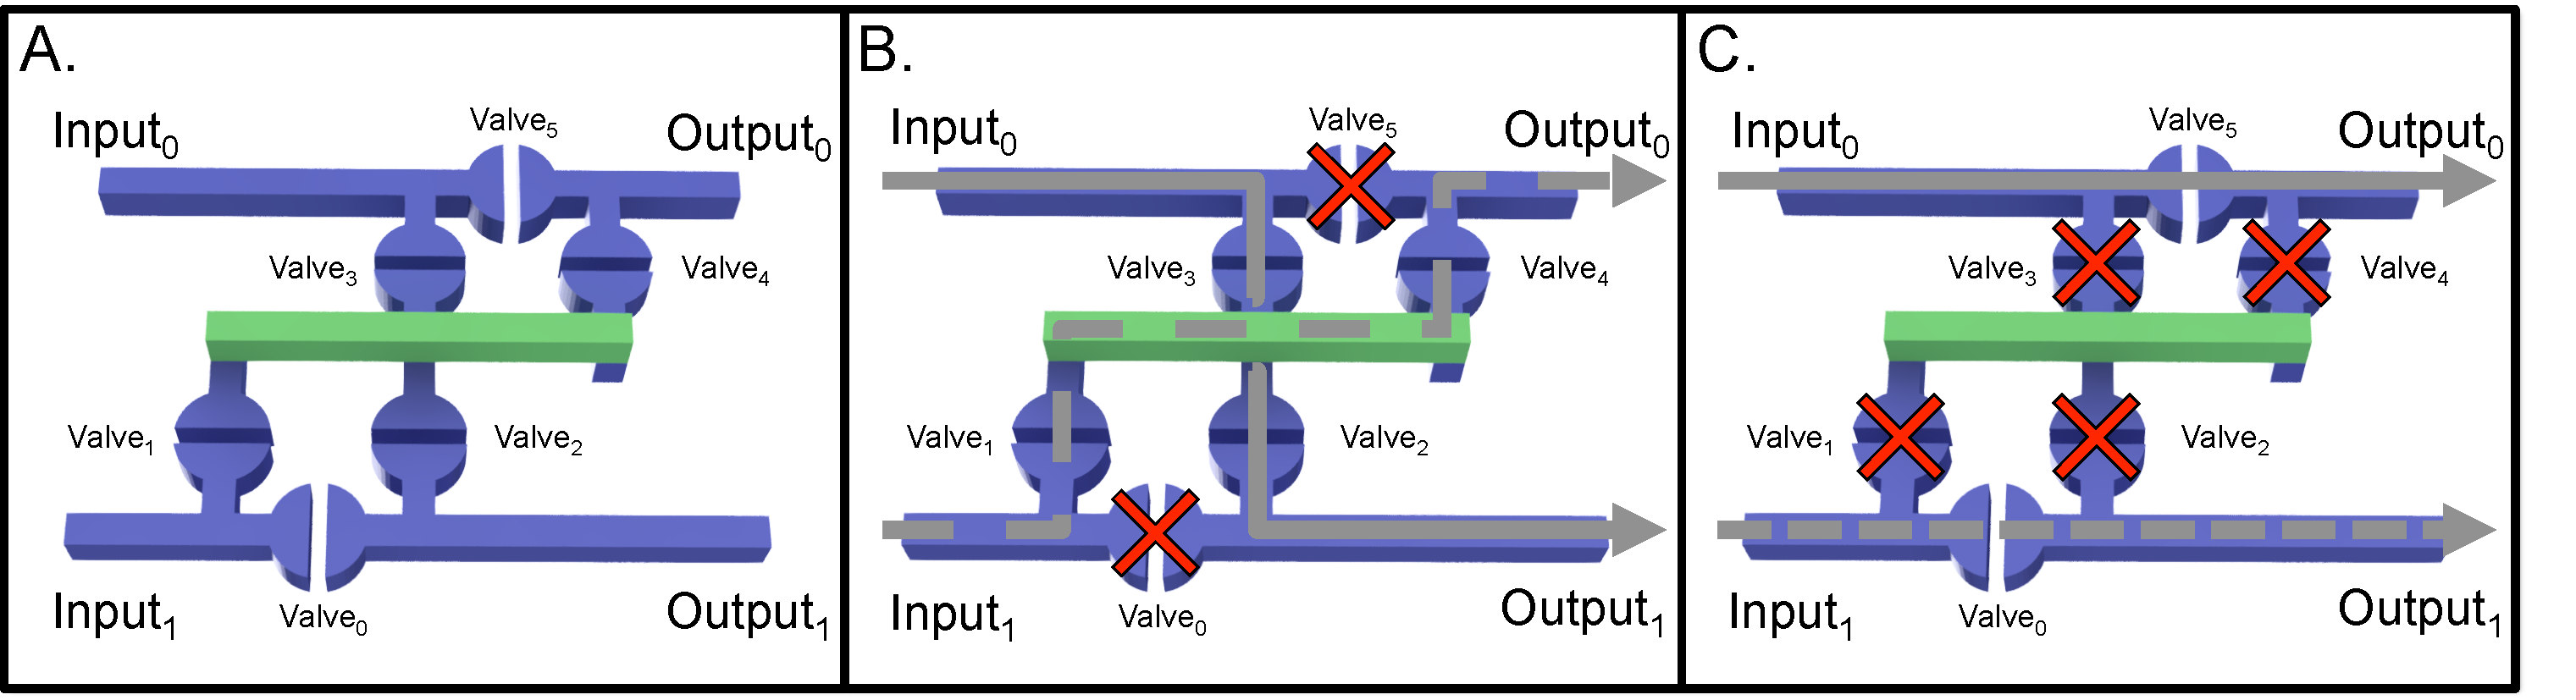
\includegraphics[width=14cm]{fig1.pdf}
    \medskip
  \end{minipage}\hfill
  \caption[Transposer theory of operation]{Theory of operation for a single transposer primitive. A. Normally closed elastomeric membrane valves are realized through discontinuities in flow channels and a corresponding pneumatic cavity on the control layer. The via (green channel) is located on the control layer and is accessed through holes punched in the PDMS membrane. Valves 0 and 5 and valves 1, 2, 3, and 4 are each driven by a single control line, thus one transposer primitive only requires two control lines. B. When valves 0 and 5 are closed and valves 1, 2, 3, and 4 are open the primitive will be in crossed mode in which the fluids will swap channels when viewed from the outputs. C. When valves 1, 2, 3, and 4 are closed and valves 0 and 5 are open the primitive will be in straight mode and fluids will flow straight through the primitive.}
    \label{fig:op}
\end{figure}

Our primitive contains six valves, each of which are not individually addressable. This is to reduce the number of pneumatic inputs required to operate the primitive allowing for greater scalability. Valves 0 and 5 in Figure \ref{fig:op} are controlled by a single control line as are valves 1, 2, 3, and 4; thus the six valves in each primitive only require two control lines for operation.

\subsection{Microfluidic Materials and Assembly}
\label{sec:assembly}
The microfluidic assembly stack for a single transposer primitive is shown in Figure \ref{fig:assembly1}. Channel and valve features were ablated from polycarbonate (PC) (McMaster-Carr, Robbinsville, NJ, USA) using a desktop CNC-mill (Othermill, Othermachine Co., San Francisco, CA, USA). The PDMS membrane was fabricated by mixing a prepolyer (Sylgard 184 Silicone Elastomer Kit, Dow Corning, Midland, MI, USA) with the curing agent at a ratio of 10:1. This mixture was then degassed in a vacuum desiccator. A 250$\mu$m thick PDMS membrane was produced using a method previously described \cite{horner2012}. The via on the control layer, shown in Figure \ref{fig:assembly1}, is accessed through holes punched in the PDMS membrane. Holes were punched by hand using a 1mm biopsy punch (Miltex, York, PA, USA). Flow and control layers were bonded to the PDMS membrane using van der Waals force as described previously \cite{mcdonald2002poly}\cite{duncan2013}. Additional bonding strength was achieved through the use of office binder clips \cite{duncan2015scaling}. The assembled PC-PDMS-PC device stack was then placed in a vacuum desiccator to remove air bubbles created at the material interfaces during assembly.
\begin{figure}[h]
  \begin{minipage}[t]{0.99\linewidth}\centering
    \includegraphics[width=9cm]{fig2.pdf}
    \medskip
  \end{minipage}\hfill
  \caption[Functional, physical, and graphical representations of a transposer]{The functional, physical and graphical representations above demonstrate how the transposer can route fluids straight through the primitive (A.) or swap the inputs when viewed from the output ports (B.). Vertices labeled $v_i$ where $v\in\{S,D,T\}$ correspond to source, decision and terminal nodes, respectively, the formal definitions for which are found in Section \ref{sec:defs}. The $i$ value for source and terminal nodes represent the vertex's level, as there will only be one of each per level, whereas the $i$ value for decision nodes are numbered incrementally by stage, left to right, starting at level 0, stage 1 as described by Algorithm \ref{alg:PopulateVertices}. The addressing node $v_o$ for the single transposer primitive represented above is $D_0$ since it is a decision node that exhibits heteroparity of coordinates (i.e., $p_l+p_s$ is an odd number).}
	\label{fig:modes}
\end{figure}

\begin{figure}[h]
  \begin{minipage}[t]{0.99\linewidth}\centering
    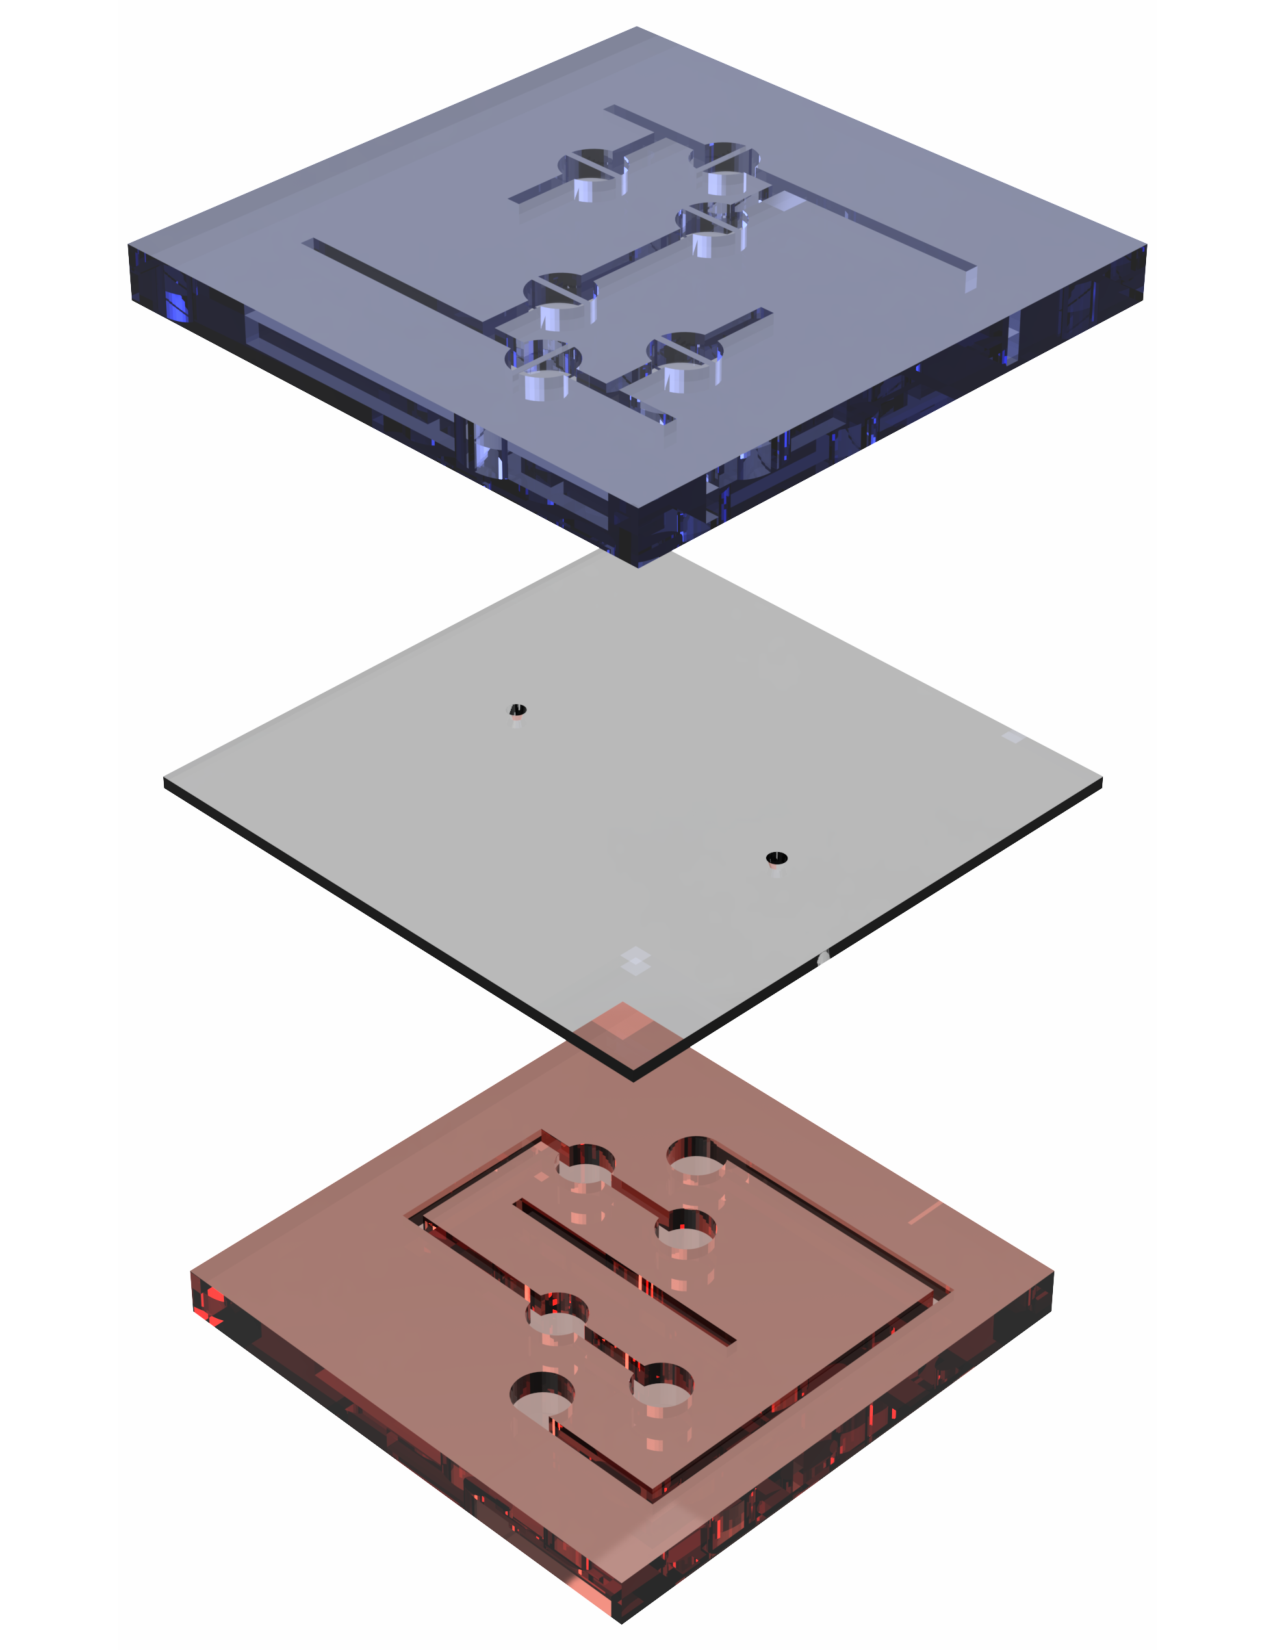
\includegraphics[width=9cm]{fig3.pdf}
    \medskip
  \end{minipage}\hfill
  \caption[Microfluidic assembly stack for a transposer]{Microfluidic assembly stack. Channel and valve geometries in flow (blue) and control (red) layers were ablated from polycarbonate. The via on the control layer is accessed from the flow layer by through-holes punched in the PDMS membrane that separates the two polycarbonate layers.}
	\label{fig:assembly1}
\end{figure}

\subsection{Routing Fabric Definitions}
\label{sec:defs}
In order to generate an algorithm that automatically routes fluids through the routing fabric to their desired destinations we begin by representing the transposer-based routing fabric as a \textbf{directed acyclic graph} (DAG). A \textbf{graph} $G=(V,E)$ is a data structure consisting of a set of \textbf{vertices} $V$ and a set of \textbf{edges} $E$ connecting these vertices \cite{vaidyanathan2015}. A \textbf{directed graph} is a subset of graphs in which all edges are ordered pairs of elements $(v_i, v_t) \in V$. An edge $e_{it}$ begins with an \textbf{initial vertex} $v_i$ and ends in a \textbf{terminal vertex} $v_t$. A \textbf{path} from $v_0$ to $v_n$ is an ordered set of edges $(v_0, v_1),(v_1,v_2),(v_2,v_3),\cdots ,(v_{n-1},v_n)$, such that the terminal vertex of each edge is the same as the initial vertex of the next edge in the path. In an \textbf{acyclic graph}, there exists no path that starts with a vertex $v_i$ and ends with the same vertex $v_i$.

An \textbf{unrouted} graph will contain all possible edges in the routing fabric, however since each individual primitive has only two modes (crossed and straight) not all combinations of edges are possible. Figure \ref{fig:algProgression}C shows an unrouted graph for a three-input fabric of transposer primitives. A \textbf{routed} graph contains only the edges used to route source nodes to the terminal nodes set by a user. Figure \ref{fig:modes} shows examples of routed graphs for a single transposer in each primitive mode, straight and crossed. A vertex is a \textbf{decision node} when it is a terminal vertex for at least one edge and an initial vertex for exactly two other edges in the unrouted graph and exactly one other edge in a routed graph. A vertex is a \textbf{source node} when it is not a terminal vertex for any edge in the graph. A vertex is a \textbf{terminal node} when it is not an initial vertex for any edge in the graph.

Each source node occupies a horizontal \textbf{level} in the graph. At a decision node, the next edge in the graph may either stay on the same level or traverse a level. The direction of the traversal (either increment a level or decrement a level) depends on the position of the vertex, as described in Section \ref{sec:unrouted}. For example, the decision node $D_0$ in Figure \ref{fig:modes} may either traverse from level 0 to level 1, thus incrementing a level, or stay on level 0, whereas the decision node $D_1$ may only traverse from level 1 to level 0, thus decrementing a level, or stay on level 1. Each vertex occupies a vertical \textbf{stage} in the graph. All edges in the graph traverse stages. For each vertex $v\in V$, $\exists$ a set of points $p=p_l,p_s$ that represent the vertex's coordinates expressed in terms of level, $l$, and stage, $s$.

Microfluidic elements are mapped onto a graph framework in order to translate the results of a graph traversal into proper fluid flow on a physical device. \textbf{Flow ports} are placed at all source (input) and terminal (output) nodes. One \textbf{control port} must be placed on each channel of equipotential in the control layer shown in Figure \ref{fig:assembly1}, with the exception of the via. Based on this requirement, each primitive requires two control ports. A \textbf {transposer primitive} $x_o$ is addressed by a single decision node $v_o \in V$. $v_o$ is said to have heteroparity of coordinates (i.e., $p_l+p_s$ is an odd number). A list of transposer primitives $X$ maintains the locations of each individual primitive $x_o$ addressed by $p_{v_{o}}$.

\section{Theory of operation}
\subsection{Scalable Routing Fabric}
A single transposer primitive can route fluids from two different input channels to two different output channels. A routing fabric, by definition, is composed of multiple transposer primitives and can be built to allow for fluid routing of $n$-input channels. The architecture on which this fabric is built is a mason layout, which can be defined as an array of primitives with either homoparity or heteroparity of coordinates; our fabric arranges primitives based on heteroparity of coordinates to account for source nodes at stage 0. The scaling of such an architecture is demonstrated in Figure \ref{fig:fabric}. The number of primitives scales according to the number of inputs, $n$, as defined by the recursively defined function in Equation \ref{eqn:fabric}. Since a single transposer primitive can route two inputs, the number of primitives required to route an $n$ less than two would be zero.

\begin{equation}
  \label{eqn:fabric}
  f(n)= \begin{cases} 0, & \mbox{if } n\mbox{ is } <2 \\ f(n-1)+n-1, & \mbox{if } n\mbox{ is } \geq 2 \end{cases}
\end{equation}

Thus, for $n\geq 2, f(n) = \sum_{i=1}^{n-1} i = n \cdot (n-1) / 2 \in \Theta(n^2).$ 

    \begin{figure}[h]
     \begin{minipage}[t]{0.99\linewidth}\centering
      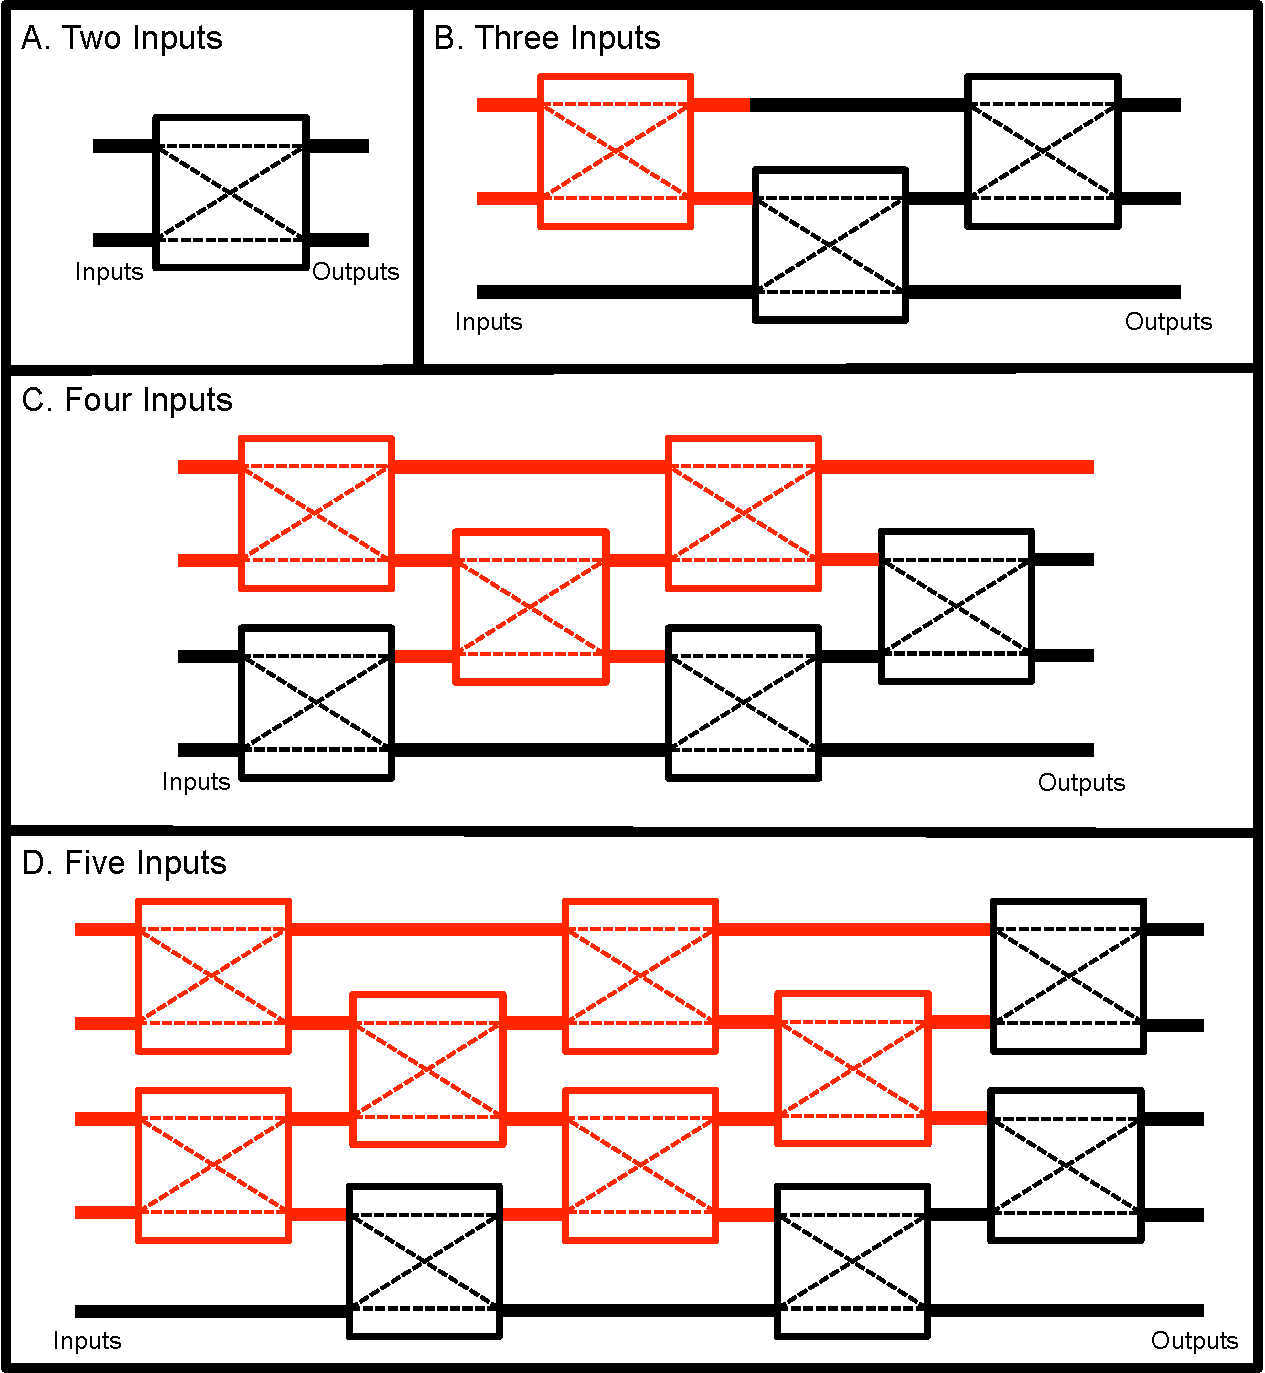
\includegraphics[width=9cm]{fig4.pdf}
      \medskip
     \end{minipage}\hfill
     \caption[Examples of a populated routing fabric]{Examples of a populated routing fabric. A. shows a single primitive, represented as a box, which is able to route two fluidic inputs to two fluidic outputs. This primitive (highlighted in red in B.) can be tiled with two other primitives, thus enabling the ability to route three fluidic inputs. The addition of three primitives (C.) to the three-input architecture (red) results in a four-input fabric. D. shows the natural continuation of the tiling process by adding four additional primitives to the four-input fabric (red) in order to create a five-input fabric. The number of transposer primitives required $f(n)$ for A--D is 1, 3, 6 and 10, respectively, as dictated by Equation \ref{eqn:fabric}.}
	    \label{fig:fabric}
    \end{figure}



\subsection{Optimality of the number of transposers}

Below, we show that a quadratic number of transposers is necessary and sufficient for routing any permutation of $n$ inputs to $n$ outputs.

\subsubsection{Necessity}

Routing an arbitrary permutation of $n$ inputs requires reordering the input fluids using transposers, in such a way that they arrive at their intended output destinations. We observe that each transposer is capable of reordering exactly two channel positions. Consider the scenario where inputs $i$ must be routed to output $n-i+1$. Here, input $i$ must require $|n-i+1-i| \in \Theta(n)$ transpositions, and therefore $\Theta(n)$ transposers. Thus, to route all $n$ input channels in this case, the problem scales on the order of $\Theta(n^2)$ transposers. It is important to note that this is a claim regarding the routing problem's complexity; the actual number of transposers required is described in Equation \ref{eqn:fabric}.

\subsubsection{Sufficiency}

Routing is accomplished by correctly routing an initial input to its destination, and then recursing. In this fashion, all inputs can be routed based on the necessary condition outlined above. The definition of correct routing is described in Section \ref{ssec:correct}.

\subsection{Planar and non planar fabrics}
Consider a graph with a vertex for each transposer and an arc from vertex $u$ to $v$ if fluid can flow directly out of the transposer corresponding to vertex $u$ into that corresponding to vertex $v$, without flowing through any  transposers along the way. It is easy to observe that this graph is planar for any $n$-input fabric. The ``intersection'' of flows occurs within a transposer. For planar fabrics, the above argument shows that the fabric design described is optimal in the number of transposers. 

\subsection{Comparison with alternative primitives}
\label{ssec:alts}
Similar programmable routing could be achieved using existing primitives. For example, a one-of-$n$ input could be routed to any of $n$ outputs using a multiplexer-demultiplexer pair with $\Theta(\lg n)$ control lines \cite{thorsen2002}. Additionally, this design would not allow for continuous-flow across all $n$ input channels, as multiplexors and demultiplexers are one-of-$n$ and $n$-of-one devices, respectively. Flow in channels not selected would, therefore, be stopped. A naive way to obtain an $n$-input $n$-output routing fabric from this would be to use $n$ mux-demux pairs resulting in $\Theta(n \lg n)$ control lines. Such a design, however, would be complex and non planar. Conversely, sub quadratic non planar fabric designs may exist, but we do not explore them here.

\subsection{Analysis of control requirements}
Since each transposer primitive requires two control lines, the number of control lines also scales on the order of $\Theta(n^2)$ with the actual number of control lines required equaling $n(n-1)$. Ballooning control requirements is a fundamental weakness of microfluidic LSI. This weakness has been largely mitigated through the use of microfluidic multiplexors \cite{thorsen2002}. The microfluidic multiplexor creates an infrastructure in which $m$ valves are controlled using $2 log_2(m)$ control lines. Thus, if a microfluidic multiplexor is integrated into to the routing fabric's control framework using latched or unlatched multiplexed addressing, as previously described \cite{melin2007}, the number of control channels would scale at $2log_2[n(n-1)]$ and as such 32 fluids could be routed with 20 control lines and the number of fluids able to be routed would increase exponentially with each additional control line (ex. 50 control lines will arbitrarily route 5,798 fluids). 
\section{Routing Algorithm}
\label{ssec:alg}
There are two main steps in our algorithm for routing within a transposer fabric:
\begin{enumerate}
	\item Generate an unrouted graph based on the number of inputs to be routed $n$
	\item Delete unnecessary edges based on desired fluid destinations to form a routed graph 
\end{enumerate}
Locations on a graph are described in terms of stages and levels. A graph for $n>2$ will have $n$ levels and $n+2$ stages, the additional two stages are a result of source and terminal nodes. Coordinates are zero-indexed. 
    \subsection{Generate Unrouted Graph}
    \label{sec:unrouted}
    Generating an unrouted graph for $n>2$ requires three primary steps:
	\begin{enumerate}
			\item Populate vertices according to rules set forth in Algorithm \ref{alg:PopulateVertices}.
			\item Assign vertices to individual transposers according to Algorithm \ref{alg:PlaceXposers}.
			\item Create edges to form an unrouted graph.
		\end{enumerate}

    \subsubsection{Populate Vertices}
    The first step in generating an unrouted graph for $n>2$ is to populate the vertices based on the number of inputs, $n$. Vertices are placed based on a set of rules. Source nodes are placed on stage 0 of each level, while terminal nodes are placed on stage $n+1$, remembering that coordinates are zero-indexed. There are two main edge cases when placing decision nodes, Level 0 and Level ($n-1$). Placing nodes on all other levels is regular as demonstrated by Algorithm \ref{alg:PopulateVertices}.

\begin{figure}
\begin{algorithm}[H]
\DontPrintSemicolon
\SetKwData{level}{level}\SetKwData{stage}{stage}\SetKwData{stages}{stages}
\SetKwFunction{AppendToV}{AppendToV}
\KwData{Number of inputs to be routed $n$}
\KwResult{A list of vertices $V$}
\Begin{
$levels \leftarrow n-1$\;
$stages \leftarrow n+1$\;
$count \leftarrow 0$\;
$V \longleftarrow \emptyset$\;
  %\tcc{Populate source and terminal nodes}
  \For{Each \level}{
	  $S_{level} \longleftarrow p=level,0$\;
	  $T_{level} \longleftarrow p=level,n$\;
	  $\AppendToV(S_{level})$\;
	  $\AppendToV(T_{level})$\;
  }
\tcc{Populate decision nodes}
  \For{Each \level}{
	  \For{\stages 1 \textbf{through} n}{
      \If{\level$= 0$ \textbf{and} \stage is odd}{
	$D_{count} \longleftarrow p=\level,\stage$\;
	$\AppendToV(D_{count})$\;
      }
      \ElseIf{\level$=n-1$}{
	      \If{$n$ is odd \textbf{and} \stage is even}{
		$D_{count} \longleftarrow p=\level,\stage$\;
		$\AppendToV(D_{count})$\;
	      }
	      \ElseIf{$n$ is even \textbf{and} \stage is odd}{
	 	$D_{count} \longleftarrow p=\level,\stage$\;
		$\AppendToV(D_{count})$\;
	      }
      }
      \ElseIf{\level$\neq 0$ \textbf{or} \level$\neq n-1$}{
	$D_{count} \longleftarrow p=\level,\stage$\;
	$\AppendToV(D_{count})$\;
      }
      Increment $count$\;
    }
  }
}
\caption{Populate Vertices. Creates vertices and assigns coordinates $p$ and type characteristics $v\in\{S,D,T\}$ to each created vertex.\label{alg:PopulateVertices}}
\end{algorithm}
\end{figure}

\subsubsection{Place Transposers}
  Individual transposers $x_o$ are addressed by a single decision node $v_o$ that exhibits heteroparity of coordinates (i.e., $p_{l_{v_o}}+p_{s_{v_o}}$ is odd). Since $v_o$ can only be of type $D$, for decision node, this excludes all vertices in stage 0 (source nodes) and stage $n+1$ (terminal nodes). Once $v_o$ is identified for all transposers in a graph, it is then possible to correctly create edges to form an unrouted graph. Algorithm \ref{alg:PlaceXposers} takes the list of vertices $V$ generated by Algorithm \ref{alg:PopulateVertices} and searches for decision nodes with heteroparity. The algorithm then creates a new transposer primitive $x_o$, assigns it an address $p_{v_{o}}$ and adds the individual transposer to the set of transposers $X$. 

\begin{figure}
\begin{algorithm}[H]
\DontPrintSemicolon
\SetKwFunction{AppendToX}{AppendToX}
\KwData{A list of vertices $V$}
\KwResult{A list of transposer objects $X$}
\Begin{
$X \longleftarrow \emptyset$\;
\For{$v \in V$ where $p_{s_v}\neq 0$ \textbf{or} $p_{s_v} \neq n+1$}{
	  \If{$p_{l_v}+p_{s_v}$ is odd}{
      $x_o \longleftarrow v$\;
      $\AppendToX(x_o)$
    }
  }
}
\caption{Place Transposers. Finds all decision nodes with heteroparity of coordinates, creates a new transposer object $x_o$ in that location and adds the new transposer to the set of transposers $X$ \label{alg:PlaceXposers}}
\end{algorithm}
\end{figure}

\begin{figure}[h]
     \begin{minipage}[t]{0.99\linewidth}\centering
      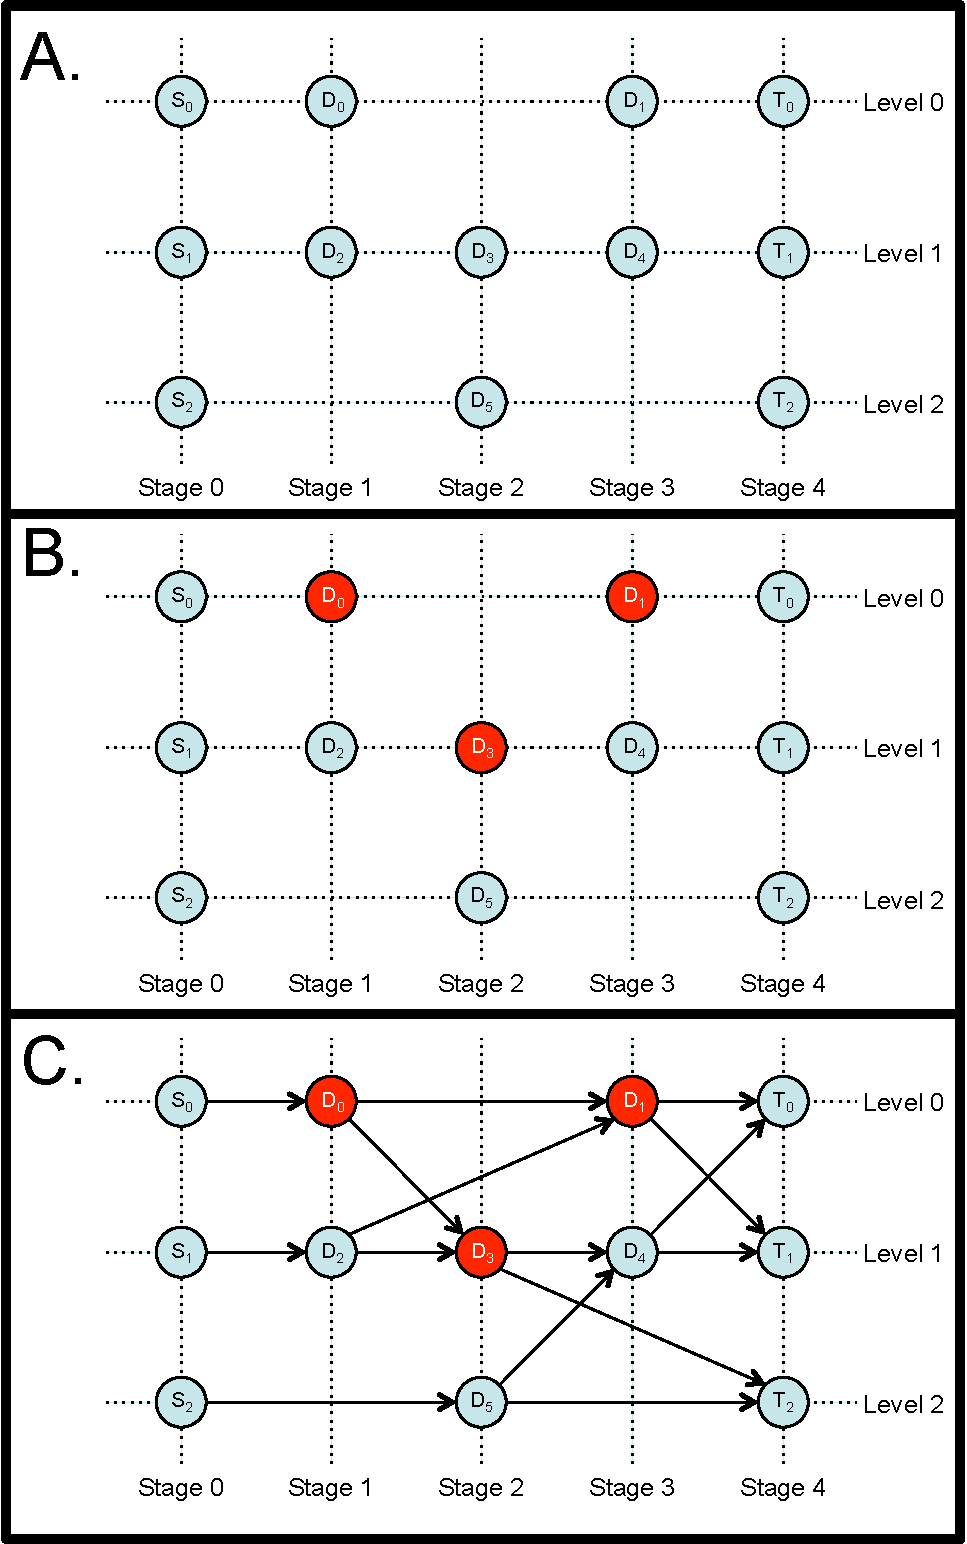
\includegraphics[width=6cm]{fig5.pdf}
      \medskip
     \end{minipage}\hfill
     \caption[Transposer routing algorithmic progression]{Algorithmic progression for generating an unrouted graph for a three-input ($n=3$) routing fabric. A. shows the outcome of Algorithm \ref{alg:PopulateVertices}, where vertices $v_i$ have coordinates $p$ and types $v\in\{S,D,T\}$ corresponding to source, decision and terminal nodes, respectively. B. shows in red the locations of the three transposer primitives as dictated by Algorithm \ref{alg:PlaceXposers}. The number of primitives is governed by Equation \ref{eqn:fabric} and the primitives are defined by their addressable node $v_o$. The graph in C. is the complete unrouted graph as dictated by Algorithm \ref{alg:GenerateGraph}.}
	\label{fig:algProgression}
\end{figure}

\begin{figure}[h]
     \begin{minipage}[t]{0.99\linewidth}\centering
      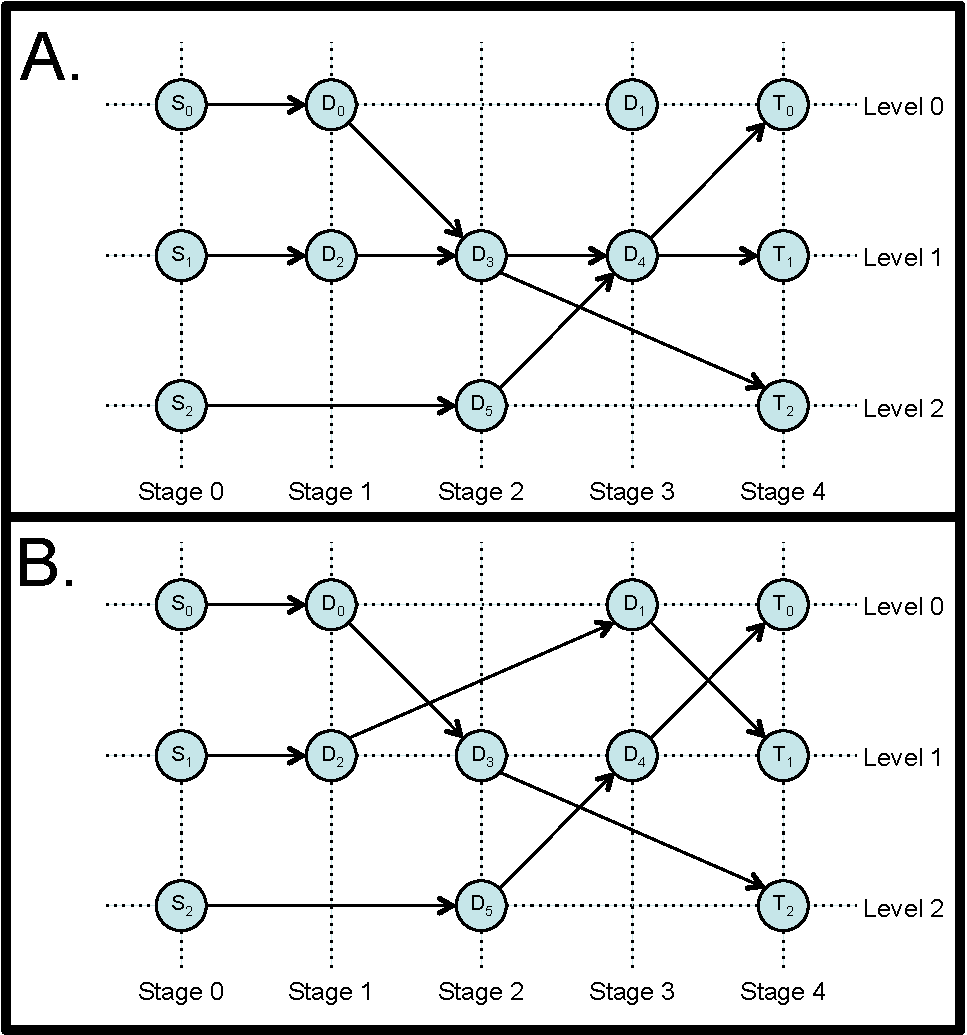
\includegraphics[width=9cm]{fig6.pdf}
      \medskip
     \end{minipage}\hfill
     \caption[Graphical representations of an illegally routed versus a correctly routed graph]{Graphical representations of illegally routed (A.) and correctly routed (B.) graphs. Each graph routes inputs from $S_0$ to $T_2$, $S_1$ to $T_1$ and $S_2$ to $T_0$. The graph in A. is illegal because vertices $D_3$  and $D_4$ appear in more than one path.}
    \label{fig:legalese}
\end{figure}


\subsubsection{Generate Unrouted Graph}
This step links the vertices in list $V$ with edges and, upon completion, results in an unrouted graph that represents a fabric of transposers for $n$ inputs. Algorithm \ref{alg:PlaceXposers} ensures that for each transposer $x\in X$, $\exists$ a decision node $v_o\in V$, and $v_o$ has the characteristic of heteroparity of coordinates; these characteristics make it possible to correctly link all vertices with edges that will form an unrouted graph representing a fabric of transposer primitives. 
    
The first edge will connect $v_o$ to the next vertex on the same level as $v_o$, i.e., $p_{l_{v_o}}$; therefore, the initial vertex for this edge will be $v_o$ and the terminal vertex will be the infimum of the set of vertices on $p_{l_{v_o}}$ with a stage number greater than $p_{s_{v_o}}$. The second edge will be the same as the first except that the terminal vertex will be the infimum of the set of vertices on the level incremented from that of $v_o$, i.e., $p_{l_{v_o}}+1$, that has a stage number greater than $p_{s_{v_o}}$. For each transposer primitive, two edges will also be added to each vertex that exists on the same stage as $v_o$, but incremented one level, i.e., $p_l+1$; we will refer to this vertex as $v_e$. The first edge will connect $v_e$ to the next vertex on the same level as $v_e$, while having a stage number greater than $p_{s_{v_e}}$. The second edge will terminate at the next vertex on the level decremented from $v_e$, which is also the same level as $v_o$, having a stage number greater than $p_{s_{v_e}}$. These steps are illustrated in Figure \ref{fig:algProgression}C and formalized in Algorithm \ref{alg:GenerateGraph}.

\begin{figure}
\begin{algorithm}[H]
\DontPrintSemicolon
\SetKwFunction{AppendToE}{AppendToE}
\KwData{A list of vertices $V$ and transposers $X$}
\KwResult{$G=(V,E)$}
\Begin{
$E \longleftarrow \emptyset$\;
\tcc{Route all source nodes to first decision node in level}
\For{$v \in V \mid p_{s_v}=0$}{
  $v_i=v$ \;
  $v_t=inf\{V \mid p_l=p_{l_v}, p_s>p_{s_v}\}$\;
  $e_{it} \leftarrow (v_i,v_t)$\;
  $\AppendToE(e_{it})$\;
}
\For{$x \in X$}{
  $v_{t_0}=inf\{V \mid p_l=p_{l_{v_o}}, p_s>p_{s_{v_o}}\}$\;
  $e_{it_0} \leftarrow (v_o,v_{t_0})$\;
  $\AppendToE(e_{it_0})$\;
  $v_{t_1}=inf\{V \mid p_l=p_{l_{v_o}}+1, p_s>p_{s_{v_o}}\}$\;
  $e_{it_1} \leftarrow (v_o,v_{t_0})$\;
  $\AppendToE(e_{it_1})$\;
  $v_e=v\in \{V \mid p_l=p_{l_{v_o}}+1, p_s=p_{s_{v_o}}\}$\;
  $v_{t_2}=inf\{V \mid p_l=p_{l_{v_e}}, p_s>p_{s_{v_e}}\}$\;
  $e_{it_2} \leftarrow (v_e,v_{t_2})$\;
  $\AppendToE(e_{it_2})$\;
  $v_{t_3}=inf\{V \mid p_l=p_{l_{v_e}}-1, p_s>p_{s_{v_o}}\}$\;
  $e_{it_3} \leftarrow (v_e,v_{t_3})$\;
  $\AppendToE(e_{it_3})$\;
}
}
\caption{Generate Unrouted Graph. Creates edges between all vertices in $V$ based on their locations on the graph and their association with transposer elements \label{alg:GenerateGraph}}
\end{algorithm}
\end{figure}

\subsection{Correctly Traverse Unrouted Graph}
\label{ssec:correct}
A routing fabric for continuous-flow microfluidics must avoid cross-contamination of fluids by ensuring that two channels do not intersect and carry a signal unless they are separated by a valve. The transposer-based routing fabric accomplishes this based on the bimodal nature of the primitive. In other words, since the primitive only has two modes, crossed and straight, and since the architecture is based on an alternating, mason grid layout, this ensures that cross contamination will never occur. 

Traversing the unrouted graph within the constraints of the primitive and architecture can be accomplished by creating paths that do not share vertices. Therefore, an \textbf{illegally routed graph} is one in which a vertex of any type appears in more than one path. An example of an illegally routed graph is shown in Figure \ref{fig:legalese}. The graph is illegal because vertices $D_3$ and $D_4$ appear in more than one path. For example, vertex $D_3$ appears in two paths: $(S_0, D_0),(D_0, D_3),(D_3,T_2)$ and $(S_1, D_2),(D_2, D_3),(D_3,D_4),(D_4,T_1)$. Therefore, traversing an unrouted graph given an ordered set of non-repeating inputs, representing the desired fluid destinations, is a matter of generating paths for each individual inputs to their desired outputs while ensuring that no paths share vertices. This process is outlined in Algorithm \ref{alg:Traverse}.

\begin{figure}
\begin{algorithm}[H]
\DontPrintSemicolon
\KwData{$G=(V,E)$, A set $D$ containing map elements $d_i$ in the from of an ordered pair of source nodes and their desired terminal node $(S_i,T_i)$}
\tcc{Ex: In Figure \ref{fig:legalese} $D=\{(S_0,T_2),(S_1,T_1),(S_2,T_0)\}$} 
\KwResult{$G'=(V,E')$, where $E'\subset E$ containing correctly routed paths $\forall d \in D$}
\Begin{
\For{$d_i \in D$}{
  Find all paths from $S_i$ to $T_i$\;
}
\For{all paths}{
  Find paths $\forall d \in D$ containing no duplicate nodes\; 
  Discard unused edges\;
  }
}
\caption{Traverse Graph. Discards unnecessary edges by setting the mode (straight or crossed) for each transposer primitive in the unrouted graph generated by Algorithm \ref{alg:GenerateGraph}\label{alg:Traverse}}
\end{algorithm}
\end{figure}

\section{Discussion}

\subsection{Primitive and Fabric}
%This work focuses primarily on the physical and algorithmic construction of a programmable fabric using multiple primitives towards flexible continuous-flow microfluidic routing. In order to demonstrate the sufficiency of our routing framework, we constructed a three-input fabric using the fabrication techniques described in Section \ref{sec:assembly}. We then implemented our algorithms in software\dag and used it to control the device. All possible permutations of three-input routes are demonstrated in Figure \ref{fig:routes}.
%No supplementary material.
This work focuses primarily on the physical and algorithmic construction of a programmable fabric using multiple primitives towards flexible continuous-flow microfluidic routing. In order to demonstrate the sufficiency of our routing framework, we constructed a three-input fabric using the fabrication techniques described in Section \ref{sec:assembly}. We then implemented our algorithms in software and used it to control the device. All possible permutations of three-input routes are demonstrated in Figure \ref{fig:routes}.

The primitive used in this work is provided simply as a means to demonstrate the functionality of the fabric. The actual architecture of the primitive used to construct the fabric is irrelevant, provided that it accomplishes the functional specification illustrated in Figure \ref{fig:modes}; thus, the fabric can be integrated with any continuous-flow microfluidic technology independent of fabrication technique and control environment. This effectively removes fluid routing considerations from chip design, thereby raising the level of abstraction, allowing experimentalists and chip designers to focus on developing functional continuous-flow microfluidic devices within the context of their particular application area. Furthermore, this work is applicable regardless of an experimentalist's existing microfluidic fabrication or control infrastructure, therefore what we present is immediately useful at no additional cost.

We acknowledge that our transposer primitive design can be optimized in many ways; for example, the primitive used in this work incorporates Manhattan geometries, which may increase transport waste and create turbulent flow patterns at right angle junctions. Manhattan geometries were chosen for clarity in demonstrating the functionality of the fabric as well as to utilize a microfluidic place-and-route tool developed in our lab \cite{huang2014}. Our fabrication methods could also be optimized with regards to materials, miniaturization, irreversible bonding, etc. Irrespective of optimizations to the primitive, the fabric in which the primitive integrates remains unchanged. In this regard, the routing fabric presented above can be integrated in any continuous-flow microfluidic technology, fabrication method or control environment regardless of the primitive's architecture or performance. 

\subsection{Comparison with Other Programmable Architectures}
This work differs from other programmable architectures, such as the recently reviewed \cite{kim2016pneumatically} class of programmable devices that consists of planar, two-dimensional valve arrays \cite{fidalgo2011}\cite{thorsen2002}\cite{jensen2013}\cite{linshiz2016end}, in its ability to achieve arbitrary continuous-flow routing while coupled with application-specific microfluidic primitives. While these two-dimensional valve array architectures present compelling cases for their ability to route, mix and store fluids, one significant shortcoming in this regard is their inability to arbitrarily route fluids while maintaining continuous flow through the device. This limitation precludes an experimentalist from using the architecture to serialize a computational work flow within a single chip architecture as described in Section \ref{sec:example}. 

The valve array architecture is proven to be an excellent platform for flexible, general-purpose microfluidic operations, to include operations other than fluid routing. The transposer-based routing architecture makes no claims as to its ability to perform any function other than algorithmically scalable, arbitrary fluid routing while maintaining continuous flow; as such, we believe our architecture consisting of a programmable routing fabric combined with application-specific (or programmable) functional blocks allows the experimentalist a maximum degree of flexibility to integrate their most-trusted microfluidic constructs into a programmable device.
\begin{figure}[h]
     \begin{minipage}[t]{0.99\linewidth}\centering
      \includegraphics[width=15cm]{fig7.pdf}
      \medskip
     \end{minipage}\hfill
     \caption[Photographs of all possible permutations for a three-input routing fabric]{All possible permutations for a three-input routing fabric. Fluid moves from left to right in each photo. The inputs from top to bottom are always in the order: green, red, blue. The outputs of the photos correspond to all possible routing permutations for the three input fluids to the three output ports.}
	\label{fig:routes}
\end{figure}



\subsection{Integration into a larger functional architecture}
Programmable routing is a key element in reconfigurable electronic computing architectures such as FPGAs \cite{compton2002reconfigurable}. An FPGA derives its basic computational abilities from configurable logic blocks (CLB), which are responsible for performing elementary logic and storage functions \cite{farooq2012tree}. More complex computations are achieved by chaining many CLBs together. An FPGA infers flexibility from the programmable nature of both the CLB and the routing fabric. Island-style FPGAs \cite{schmit2005extra} are a particular FPGA architecture that organize CLBs in a two \cite{chang1996universal} or three dimensional \cite{alexander1995three} array connected by a grid of prefabricated wire segments and programmable routing structures \cite{chang1996universal}. The CLBs can be viewed as computational ``islands'' among an ocean of routing elements \cite{farooq2012tree}, as shown in Figure \ref{fig:fpgaArchAndRouting}A. 

\begin{figure}[h]
     \begin{minipage}[t]{0.99\linewidth}\centering
      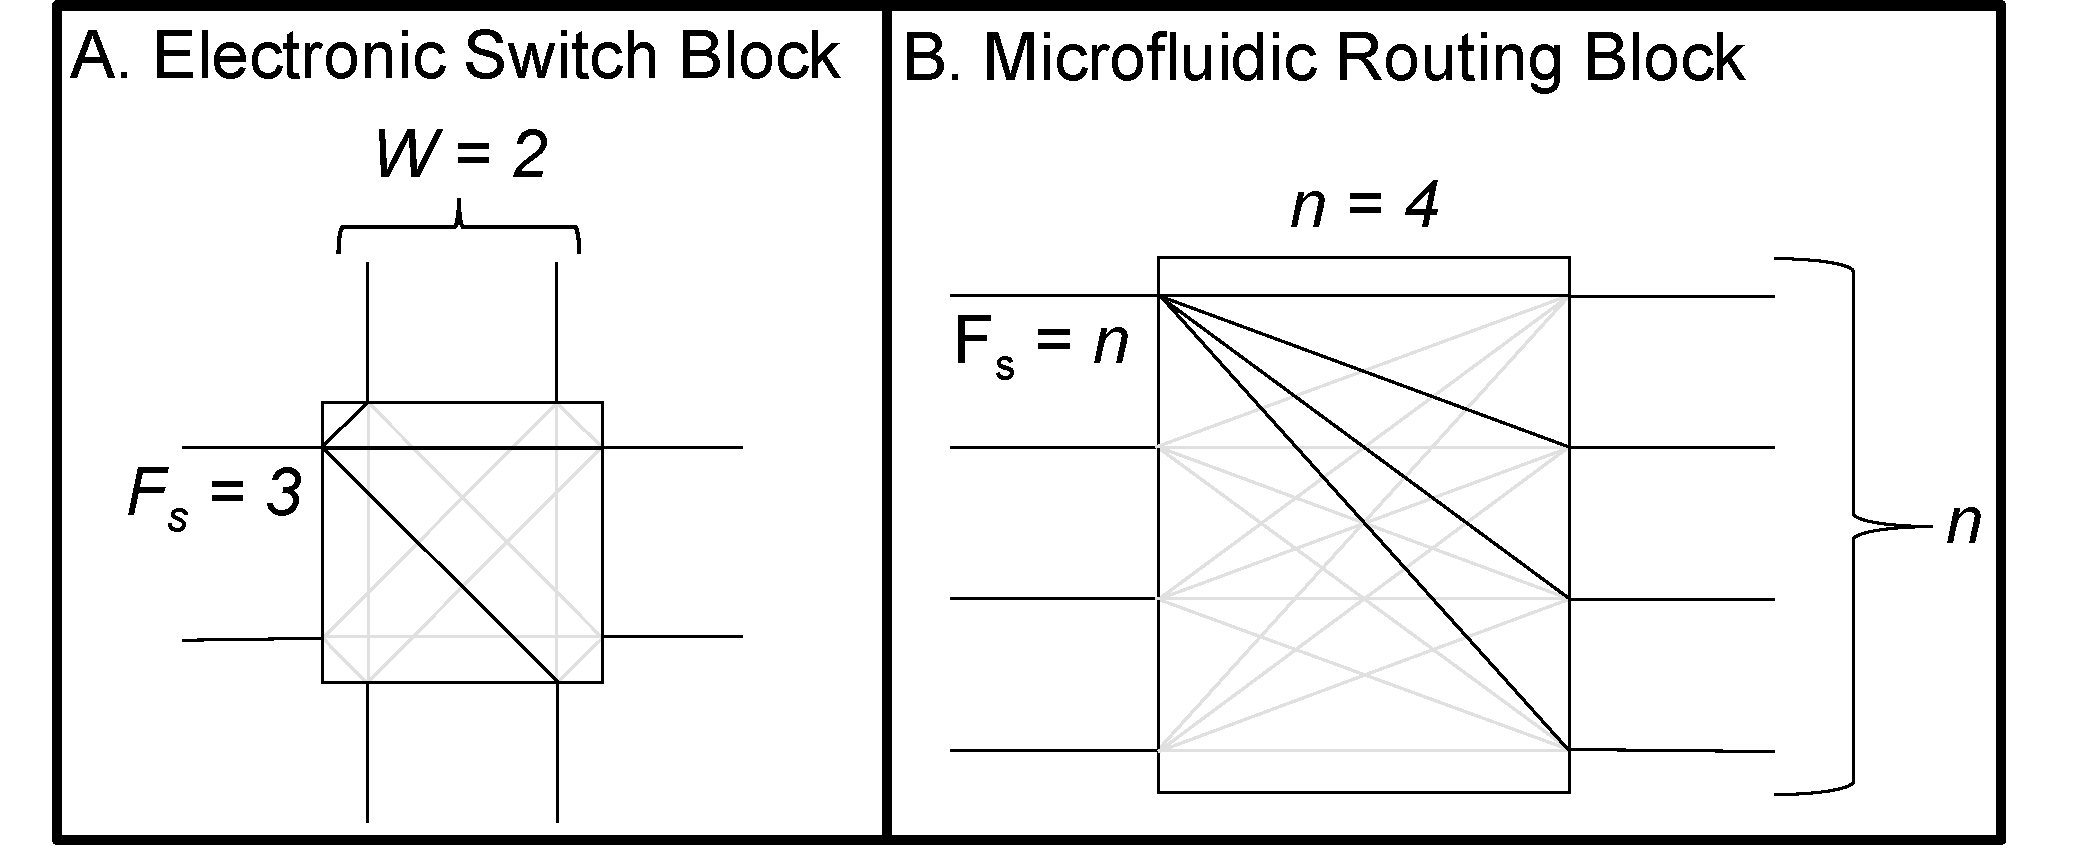
\includegraphics[width=15cm]{fig8.pdf}
      \medskip
     \end{minipage}\hfill
     \caption[Electronic and Microfluidic programmable routing blocks]{Electronic (A.) and Microfluidic (B.) programmable routing blocks. The channel width ($W$) and flexibility ($F_s$) of the electronic switching block (A.) is two and three, respectively. These switching block attributes are the same as the ones used in Figure \ref{fig:fpgaArchAndRouting}A and \ref{fig:fpgaArchAndRouting}B.}
	\label{fig:switchBlocks}
\end{figure}

Programmable routing structures within an island-style FPGA can take on one of two general forms: \textbf{switching blocks} or \textbf{connection blocks}. Connection blocks are used to connect the prefabricated wire segments directly to CLBs. Switching blocks are used to connect prefabricated wire segments at dimensional intersections within the 2D or 3D array; for example, a 2D island-style FPGA architecture places a switching block at all intersections of vertical and horizontal prefabricated wire segments \cite{schmit2002fpga}, as Figure \ref{fig:fpgaArchAndRouting}A demonstrates. As shown in Figure \ref{fig:switchBlocks}, $W$ denotes the number of prefabricated wire segments on each side of the switching block, while $F_s$ denotes the switching block's flexibility, i.e., the number of possible routes for each prefabricated wire segment entering the switching block. Figure \ref{fig:fpgaArchAndRouting}B is an example of signal routing using a switching block with $W=2$ and $F_s=3$. 


A transposer-based routing fabric can be viewed as having the functionality of a combination switching block and connection block, which we will call a \textbf{routing block}, in a 1D FPGA. A microfludic routing block can be described in the same terms as an FPGA switching block. As shown in Figure \ref{fig:fpgaArchAndRouting}C, the routing block developed in this work has a flexibility $F_s=n$ and width $W=n$. Microfluidic \textbf{functional blocks} can take the form of any microfluidic primitive such as cell traps, gradient generators, or optical reporting areas. These functional blocks need not be uniform with regard to the number of input or output ports between blocks, nor must they be symmetric in the number of input and output ports in the same block, as Figure \ref{fig:fpgaArchAndRouting}C shows. Functional blocks may take on any class of microfluidic function including, but not limited to, combining operations (mixing, droplet generation, etc.), biological operations (cell culture, polymerase chain reaction (PCR), etc.), or measurement/sensing operations (microscopy, pH, etc.). 

In microfluidic and electronic FPGA architectures, elementary functions are performed in functional blocks and CLBs, respectively. More complex operations are accomplished by chaining multiple blocks together using our routing fabric. Since all elements are modular and programmable, both architectures provide flexibility that is impossible to achieve in traditional, application-specific chips.  Chaining multiple primitives through microfluidic routing blocks has compounding effects on a chip's flexibility and functional capability in a manner similar to that of an FPGA. This concept is described in further detail in Section \ref{sec:example}. These novel capabilities are impossible in a continuous-flow microfluidic device without the capability of dynamic fluid routing provided by the transposer routing fabric.


\subsection{Example Architecture}
\label{sec:example}
Consider a lab that utilizes two distinct microfluidic devices. The first device is a two-stage microfluidic designed to mix a particle stream with a buffer stream and then perform separation as part of a protocol for rare cell isolation \cite{pamme2007continuous}. The second device is also a two-stage microfluidic but instead of performing mixing and separation, this device utilizes cell trapping followed by a thermal treatment within a temperature-controlled reaction chamber as part of a polymerase chain reaction (PCR) protocol \cite{zhang2006pcr}. If these two distinct chips are brought together, with a single transposer separating the two stages, a flexible architecture is created with novel functionality. For example, the two independent chips were originally only capable of mixing followed by separation and trapping followed by temperature cycling, respectively; the new chip, incorporating a single transposer, is now capable of mixing followed by temperature cycling, which could be useful in chemical synthesis \cite{jensen2014tools}, and at the same time is capable of trapping followed by separation, which is part of a protocol for debulking platelets from blood samples \cite{shields2015microfluidic}.

	Figure \ref{fig:example} shows a schematic representation of all possible functionalities derived from such an architecture. The addition of more functional blocks vertically (i.e., increasing $n$ on a routing block) increases the number of possible simultaneous operations the chip can perform, while adding more functional blocks horizontally, with each stage separated by a routing block, increases the number of possible sequential operations. This specificity achieved through well-tested and characterized functional blocks (ex., mixers, separators, cell traps and reaction chambers) coupled with the flexibility of a programmable routing architecture unlocks a new category of programmable devices made possible only through arbitrary, continuous-flow microfluidic routing. 


Functional blocks may have incompatible channel geometries relative to other functional blocks in a larger architecture. This issue can be mitigated by modifying the primitive's channel geometries for each differing channel of interest. This would only be necessary should a channel reduction or expansion impede function and if the differing channels require rerouting; otherwise, these geometries would be considered internal to a functional block and not part of the routing fabric. Should a chip architecture require rerouting of multiple channels of differing dimensions, this would result in separate routing fabrics for each channel geometry that requires rerouting. The routing fabric is flexible such that a device containing separate routing fabrics, based on channel dimensions, could be integrated without any modifications to the algorithmic framework.

\begin{figure}[h]
  \begin{minipage}[t]{0.99\linewidth}\centering
    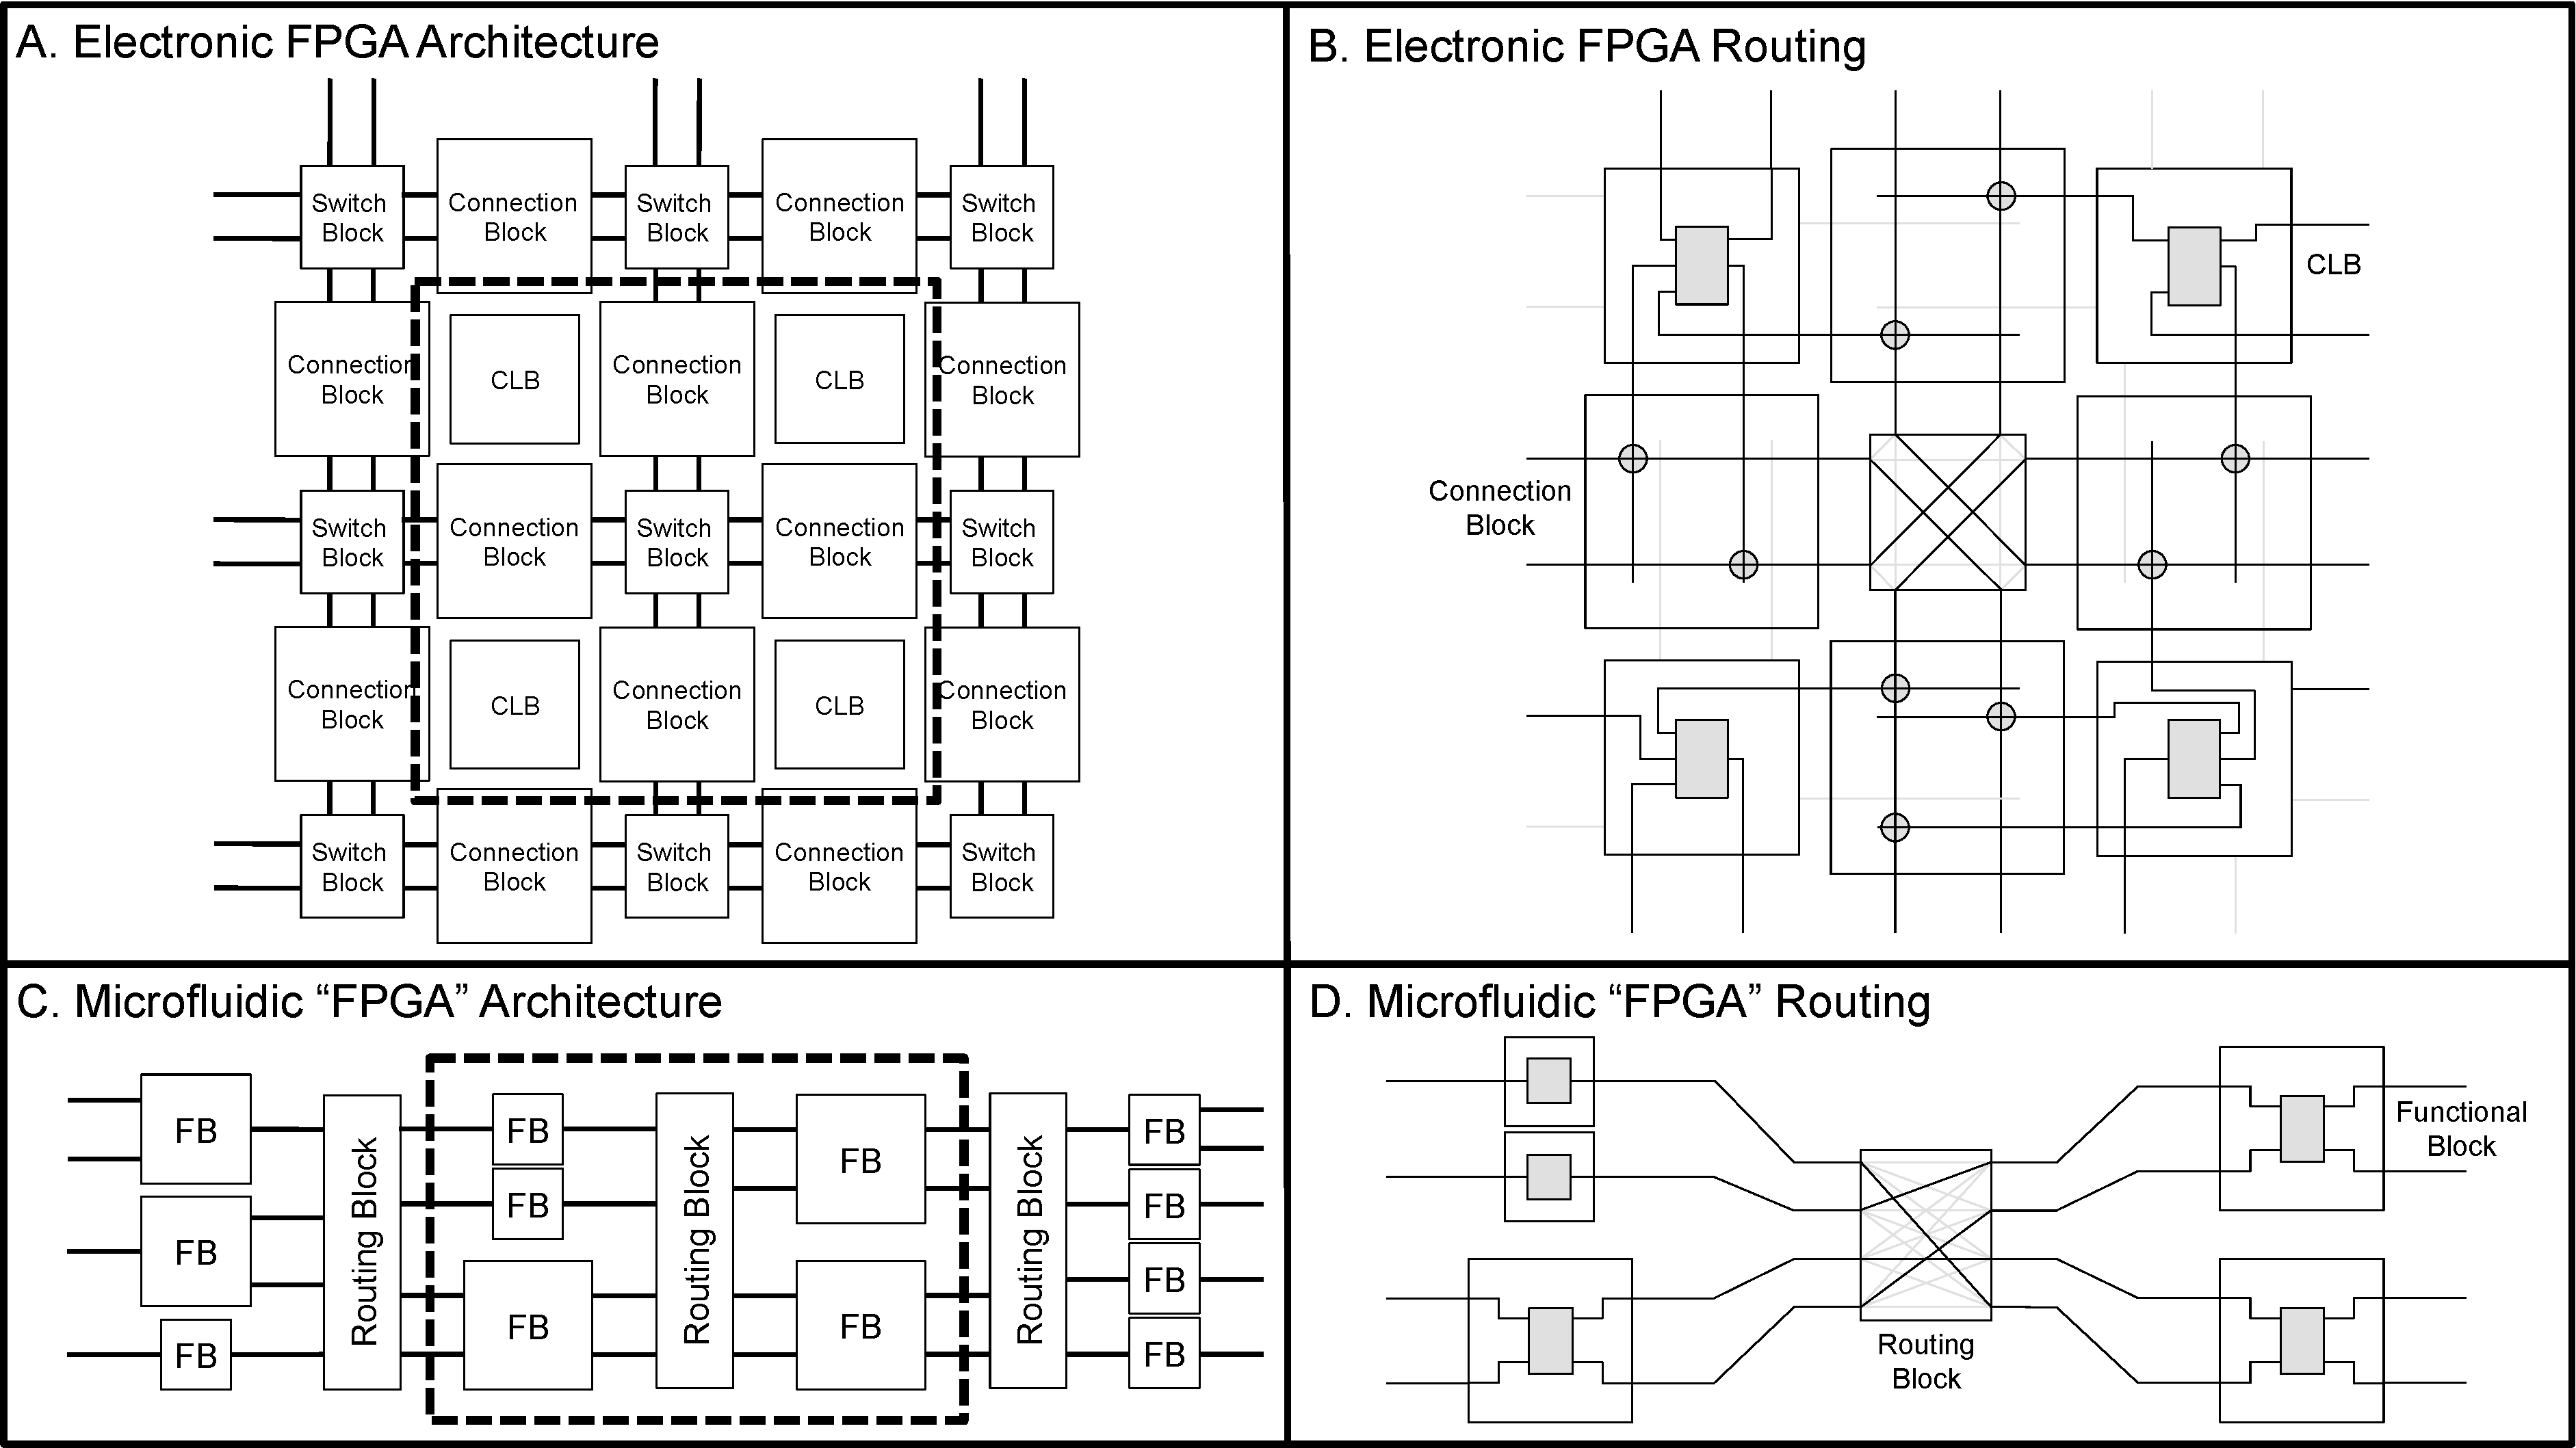
\includegraphics[width=15cm]{fig9.pdf}
    \medskip
  \end{minipage}\hfill
  \caption[Electronic and Microfludic programmable architectures]{Electronic and Microfluidic programmable architectures. A 2D, island-style Electronic FPGA architecture (A.) with example routing (B.) of the area of interest indicated by a dashed line in A. A transposer-based microfluidic chip architecture (C.) with example routing of area of interest (D.) indicated by a dashed line in C. Microfluidic functional blocks (FB) can be any continuous-flow microfluidic function such as mix, measure, etc. The microfluidic architecture in C. demonstrates that functional blocks need not be uniform (i.e., all have the same number of input/output channels). Grey lines in B. and D. indicate unconnected paths.}
	\label{fig:fpgaArchAndRouting}
\end{figure}
\subsection{Dynamic Reconfiguration}
Integrating intermediate sensing operations as functional blocks within a transposer-based microfluidic routing architecture unlocks a unique ability to dynamically reroute fluids based on real-time measurements. This is particularly valuable in experiments involving fluidic operations that depend on dynamic fluidic variables such as directed evolution \cite{wang2014microfluidic}, refinement \cite{swain2013thinking} and genetic logic \cite{tamsir2011}. However, reconfiguration of the routing fabric during run time carries a distinct limitation whereby at the moment of reconfiguration, a contaminated plug of liquid will propagate through the device. The problem is analogous to the concept in digital electronics of a dynamic discipline \cite{Harris+Harris}. The dynamic discipline affirms that the output of a digital logic element (ex. a flip flop) is not deterministic if queried inside of its established propagation delay. Extending this analogy to microfluidic routing, it can be stated that if a transposition occurs within channels containing functionally orthogonal fluids (so as to prevent permanent contamination downstream) that the output of the system will be valid only after waiting for the contaminated plugs to propagate through the device.
\begin{figure}[h]
     \begin{minipage}[t]{0.99\linewidth}\centering
      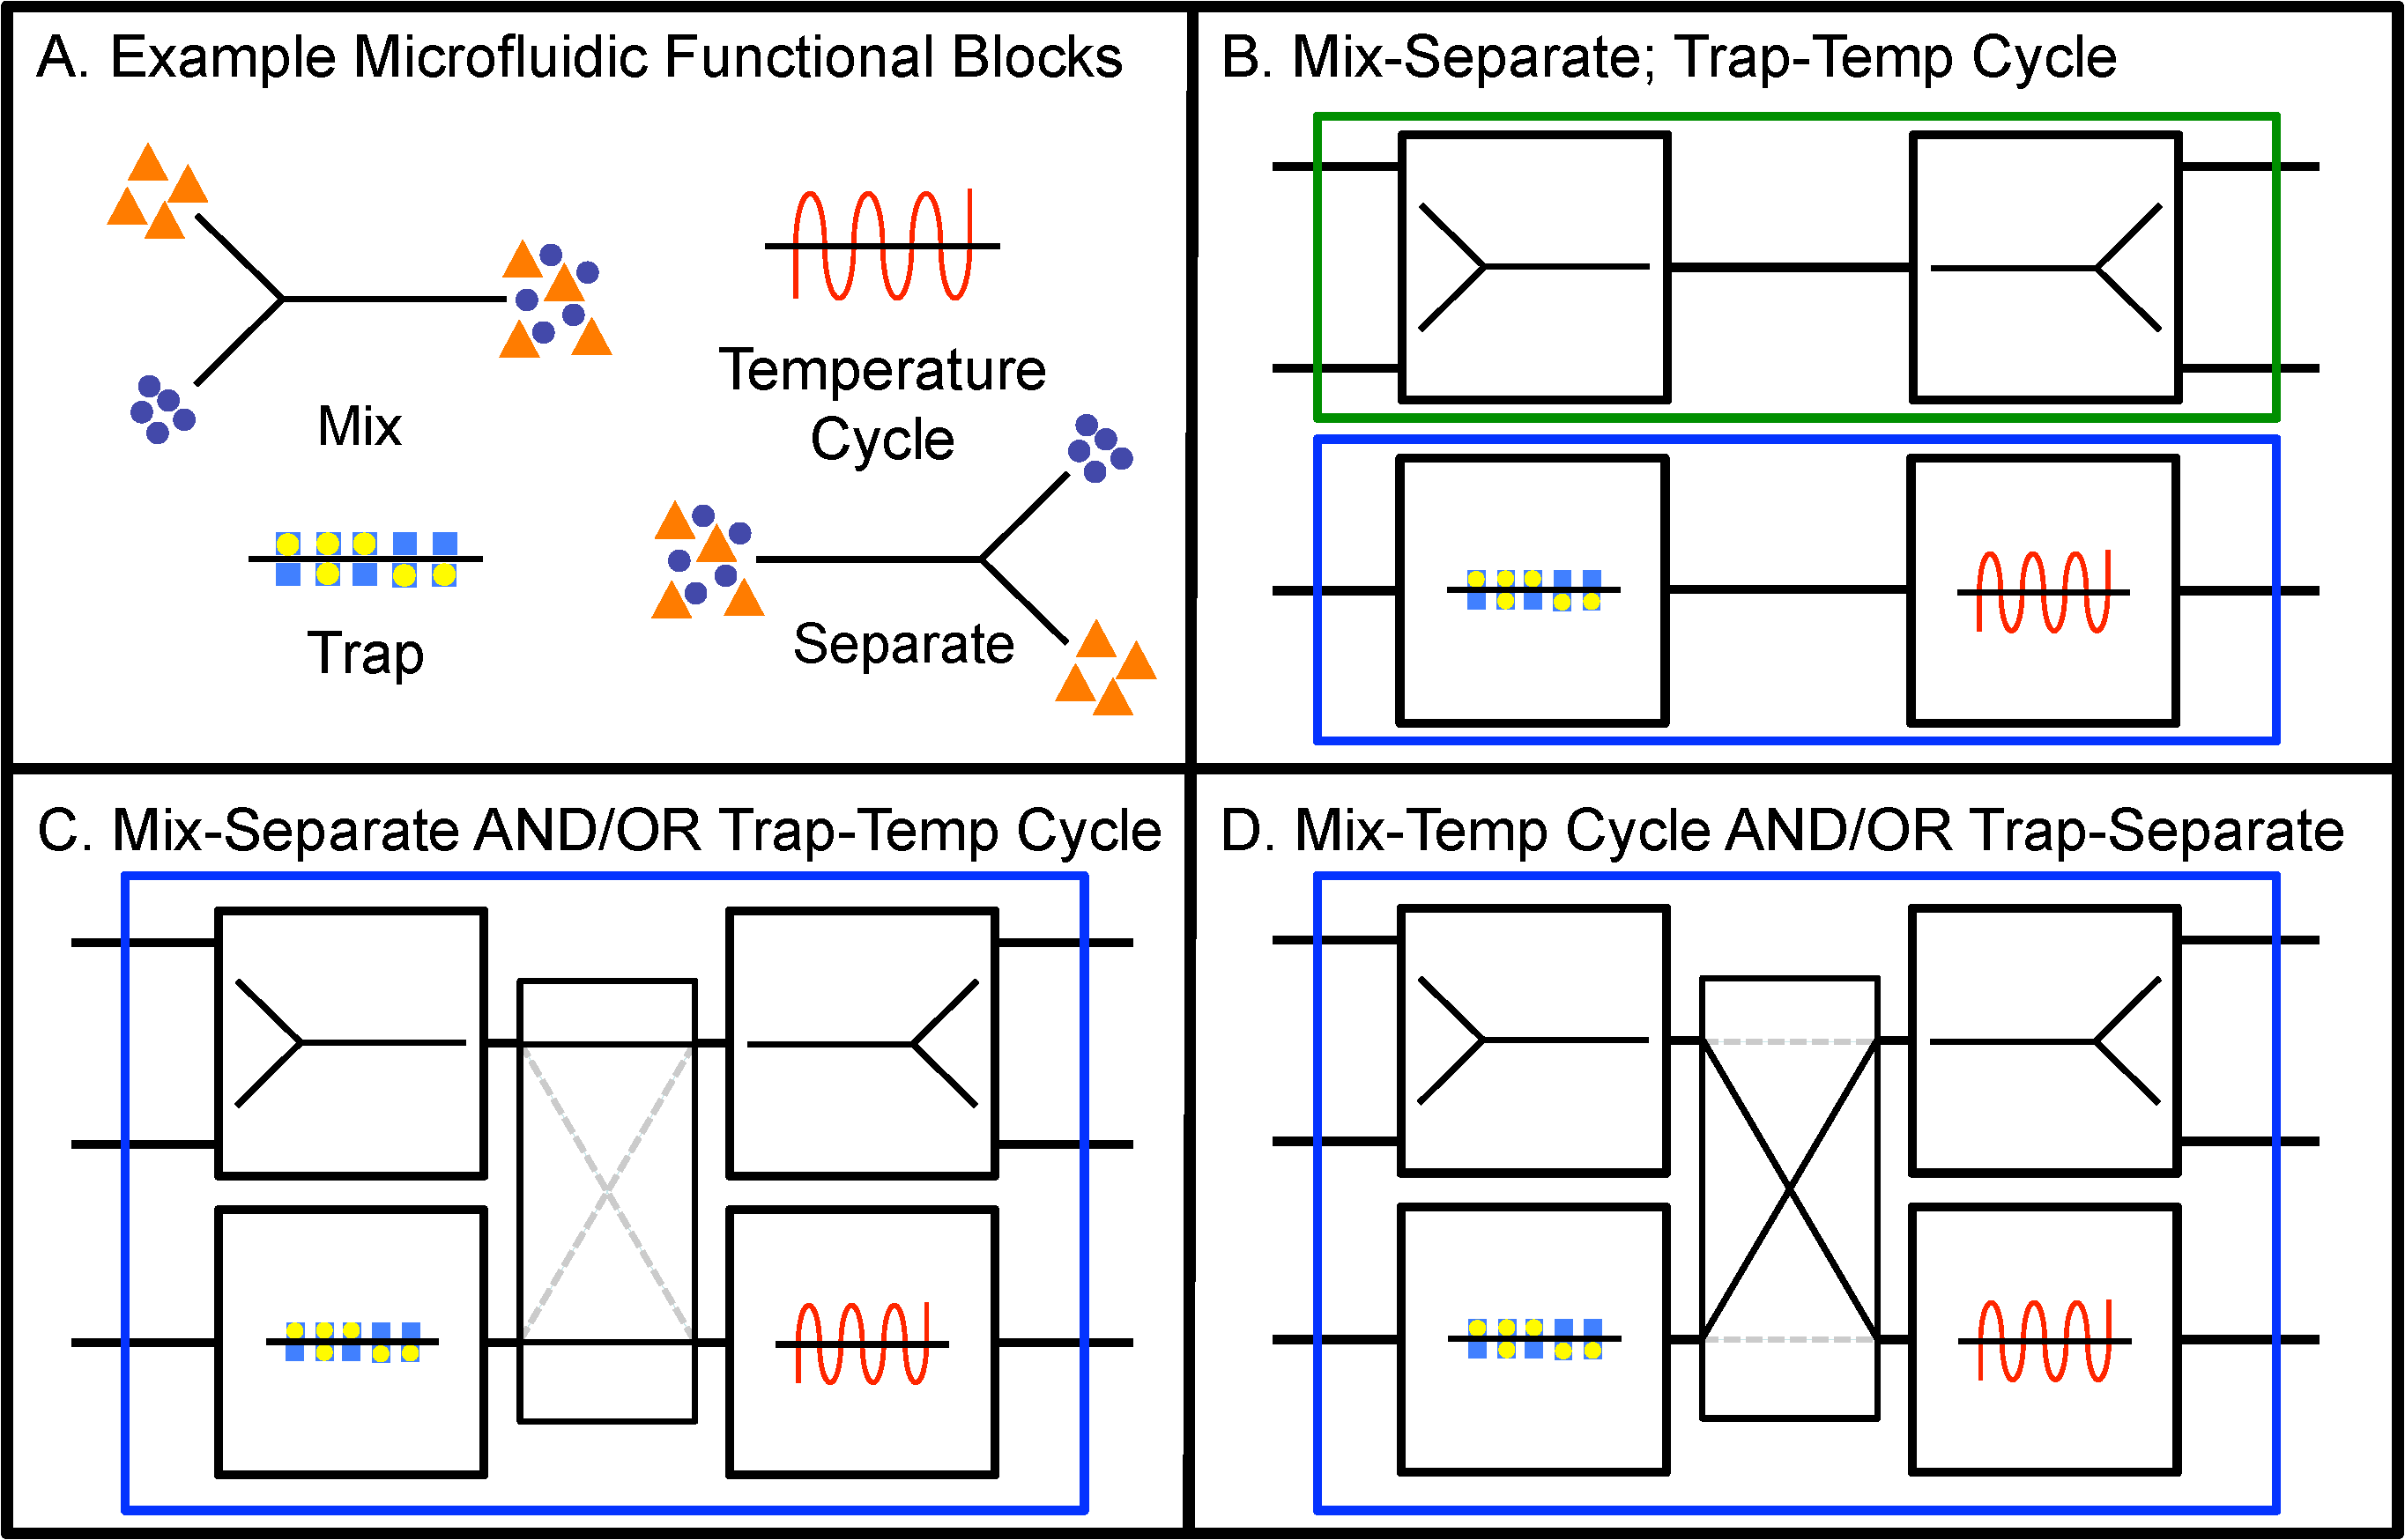
\includegraphics[width=14cm]{fig10.pdf}
      \medskip
     \end{minipage}\hfill
     \caption[Example of a functional, programmable microfluidic architecture]{Example architecture utilizing a single transposer. Microfluidic functional blocks (A.) are connected via static channels to form two separate devices (B.) the functions of which are immutable. One device can perform mixing and then separation, while the other can perform cell trapping and then temperature cycling. A transposer is used to join the functional blocks in lieu of static channels (C. and D.). This results in two novel functions, mix then temperature cycle and trap then separate (D.). Additionally, The single microfluidic chip is able to perform both functions shown in C. simultaneously as well as both functions in D.}
	\label{fig:example}
\end{figure}



\subsection{Future Work}
One particular strength of this work is the technology-agnostic manner in which the framework was built. This means that the transposer primitive can be optimized to suit any control or fabrication environment so long as the basic functionality shown in Figure \ref{fig:modes} is retained. The optimal transposer primitive may look dramatically different between experimentalists performing separation using acoustophoresis \cite{petersson2007free} versus filtration \cite{pamme2007continuous}, yet the routing framework would be identical.

Since each primitive only requires two control lines, which are of equipotential and toggled in a manner similar to the microfluidic multiplexor previously described \cite{thorsen2002}, the optimization of control lines based on variable routing constraints is a solvable problem.

Finally, the formulation of a flexible microfluidic architecture that encompasses a maximum subset of microfluidic assays is under development. This chip would allow experimentalists to fabricate devices in bulk, yet maintain maximum flexibility to perform a large range of assays and experiments using the same chip. Organic software will accompany this architecture and serve to integrate device-level microfluidic control with assay-level specification. This effectively raises the level of abstraction for the microfluidic experimentalist and frees the community from the need to design, fabricate and control singular microfluidic architectures for each experiment; rather, the experimentalist will reprogram the same chip architecture for many types of experiments through the same control environment.

\section{Conclusions}
This work demonstrates a novel microfluidic routing fabric for continuous-flow devices using a scalable primitive called a transposer. The fabric exists independent of any optimizations made to the primitive itself. We proved that fluidic routing through the fabric is extensible and developed algorithms to do so. We then integrated the fabric into a larger architecture towards the development of a programmable continuous-flow microfluidic device akin to the class of electronic devices known as FPGAs. 

The barrier to entry for continuous-flow microfluidics can be prohibitively high, yet the benefits of microfluidic technology are too good to ignore \cite{whitesides2006}. This work serves to introduce a new class of programmable microfluidic devices aimed at decreasing the design, fabrication and operational costs of continuous-flow microfluidics thus increasing the accessibility of microfluidic technology. It is our hope that programmable continuous-flow microfluidics could serve as the catalyst towards microfluidic ubiquity as programmable electronics was for electronic computing.

\cleardoublepage

% -------------------------------------
% CHAPTER 4: Acoustophoresis
% -------------------------------------
\chapter{Rapid prototyping of parameterized acoustofluidic microchannels towards isolation of bacteria for point of care diagnostics}
\label{chapter:acoust}
\thispagestyle{myheadings}

% set this to the location of the figures for this chapter. it may
% also want to be ../Figures/2_Body/ or something. make sure that
% it has a trailing directory separator (i.e., '/')!
\graphicspath{{4_acoust/Figures/}}

\section{Introduction}
\label{sec:acoust_intro}
Acoustic manipulation has emerged as a versatile method for microfluidic separation and concentration of particles and cells. Most recent demonstrations of the technology use piezoelectric actuators to excite resonant modes in silicon or glass microchannels. Here, we focus on acoustic manipulation in disposable, plastic microchannels in order to enable a low-cost processing tool for point-of-care diagnostics. Unfortunately, the performance of resonant acoustofluidic devices in plastic is hampered by a lack of a predictive model . In this manuscript, we build and test a plastic blood-bacteria separation device informed by a design of experiments approach, parametric rapid prototyping, and screening by image-processing. We demonstrate that the new device geometry can separate bacteria from blood while operating at 275\% greater flow rate as well as reduce the power requirement by 82\% , while maintaining equivalent separation performance and resolution when compared to the previously published plastic acoustofluidic separation device. 

\section{Problem Statment}
\label{sec:acoust_ps}
Separation and concentration of particles and cells via microfluidic acoustic manipulation has emerged as a versatile method for rapid and efficient fluid processing. It is an attractive alternative over other fluid manipulation techniques because it is label-free, requires no electrodes or specialized structures in the microchannel, and has the potential for scale-up for high throughput processing \cite{antfolk2017continuous}\cite{bhagat2010microfluidics}. In so-called ``bulk'' acoustic microfluidic devices, the acoustophoretic force is maximized  as the fluid-filled microchannel resonates as a cavity and establishes a standing pressure wave transverse to flow.  Hence, the magnitude of the acoustic force on a particle depends strongly on the physical dimensions of the channel and walls, which must be appropriately selected for the ultrasonic excitation frequency \cite{bruus2012acoustofluidics}. 

The force exerted on a particle by the acoustically-driven standing pressure wave scales cubically with particle diameter \cite{settnes2012forces}. Thus, acoustic manipulation is particularly well suited for isolating bacterial samples from larger blood components such as red blood cells (RBCs) and white blood cells (WBCs) based purely on relative differences in size \cite{ohlsson2016integrated}\cite{li2016acoustofluidic}. This is useful as downstream assays, such as antimicrobial susceptibility testing, benefit from a purified, well-defined input with reduced contamination of mammalian cell components.

Silicon, glass, or metal devices are commonly used for acoustophoresis because the rigid channel walls provide a near ideal acoustic boundary against the sample fluid, enhancing the required standing wave resonance \cite{barnkob2009acoustofluidics}\cite{hill2008modelling}. This ideal boundary simplifies design because one-dimensional analysis can be used to estimate the resonant modes in the channel-fluid system. However, the rigid materials used in these devices are relatively expensive and slow to manufacture, have limited compatibility with many biological samples, and pose challenges to produce as disposable laboratory tools \cite{nge2013advances}.  On the other hand, our recent work has demonstrated acoustophoresis in plastic, showing that acoustic separation of RBCs is possible in polystyrene, opening the door to low-cost diagnostic and therapeutic devices \cite{mueller2013continuous}.


However, the design of optimized plastic acoustofluidic devices is hampered by complex boundary conditions relative to those of more rigid materials, and a satisfactory predictive model is not yet established, because the one-dimensional approximations are inaccurate and the channel walls can no longer be considered ideally rigid \cite{mueller2013continuous}.  Moreover, even for rigid materials, a sophisticated two-dimensional analysis does not appear to easily predict experimental performance in detail \cite{garofalo2016performance}\cite{bora2015efficient}. To further optimize the geometry of acoustic microfluidics in plastic, a parametrized experimental investigation provides an expanded database for comparison with simulation and can give performance improvements without the need for simulation.  

This study used rapid prototyping, statistical design of experiments, and rapid experimental screening to obtain a better-performing device geometry when compared to the only other plastic, acoustofluidic blood--bacteria separation device in literature \cite{mueller2013continuous}, which will be referred to as the \textit{baseline}. The baseline was designed in accordance with the existing one-dimensional hard-wall theory and no further optimization had been attempted. The devices tested varied in cross section dimensions. 

While plastic acoustofluidic devices can be produced in volume using methods such as hot embossing or injection molding \cite{heckele2003review}, prototyping test geometries in small batches could become a costly endeavor.  We minimized fabrication costs by manufacturing chips on-site through the use of an automated, rapid prototyping software framework in conjunction with a new class of inexpensive, desktop computer numerical controlled (CNC) micromills.

%\begin{figure}[htb]
  %\begin{minipage}[t]{0.99\linewidth}\centering
    %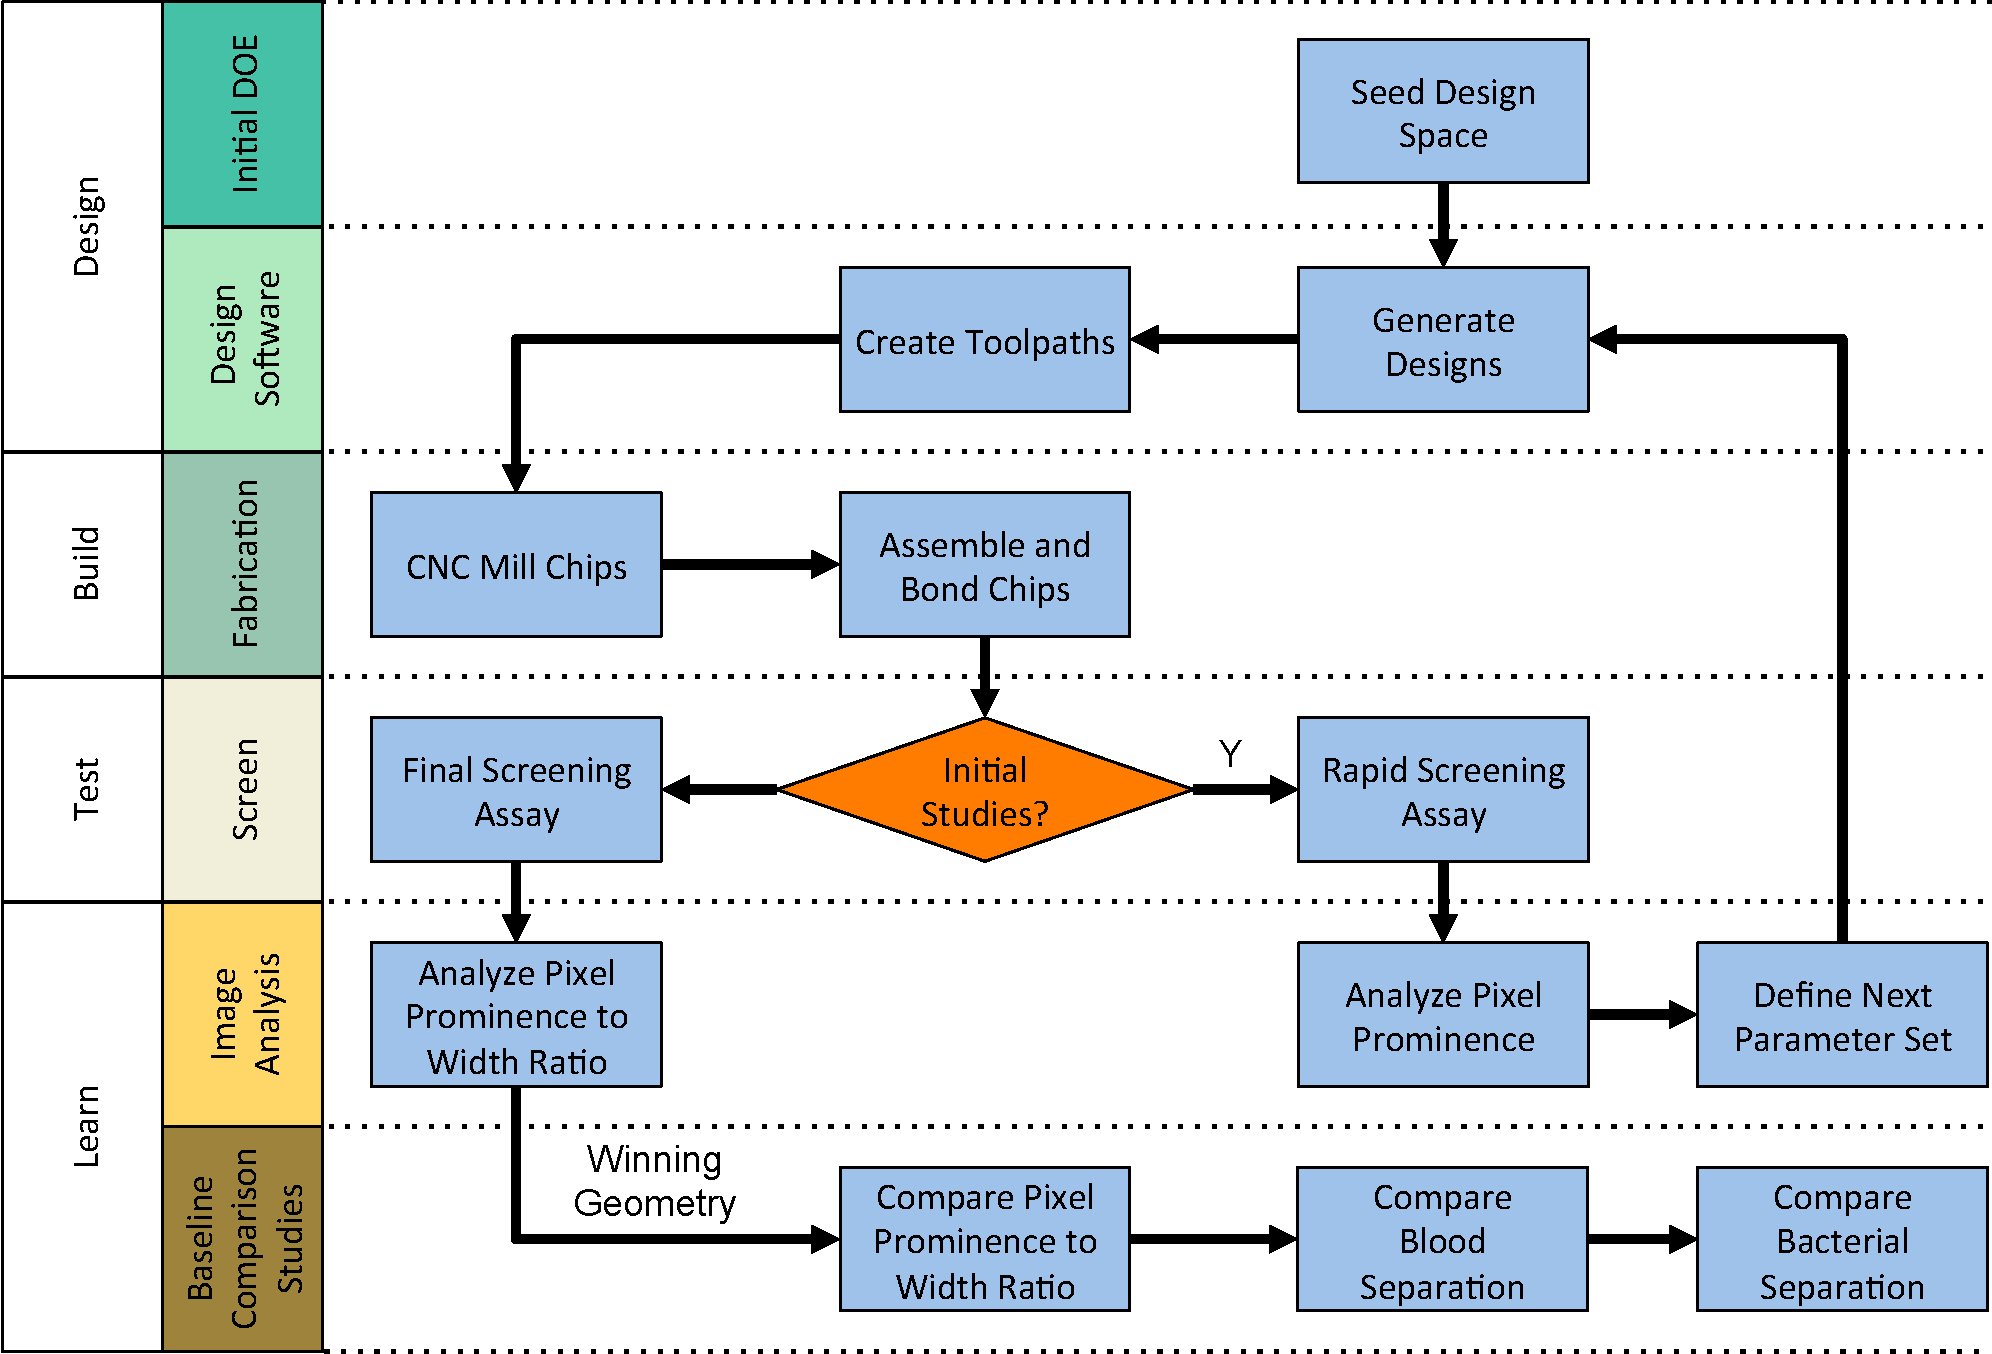
\includegraphics[width=14cm]{flow.pdf}
  %\end{minipage}\hfill
%\caption{Rapid Prototyping Workflow.}
%\label{fig:flow}       % Give a unique label
%\end{figure}


\begin{figure}[htb]
  \begin{minipage}[t]{0.99\linewidth}\centering
    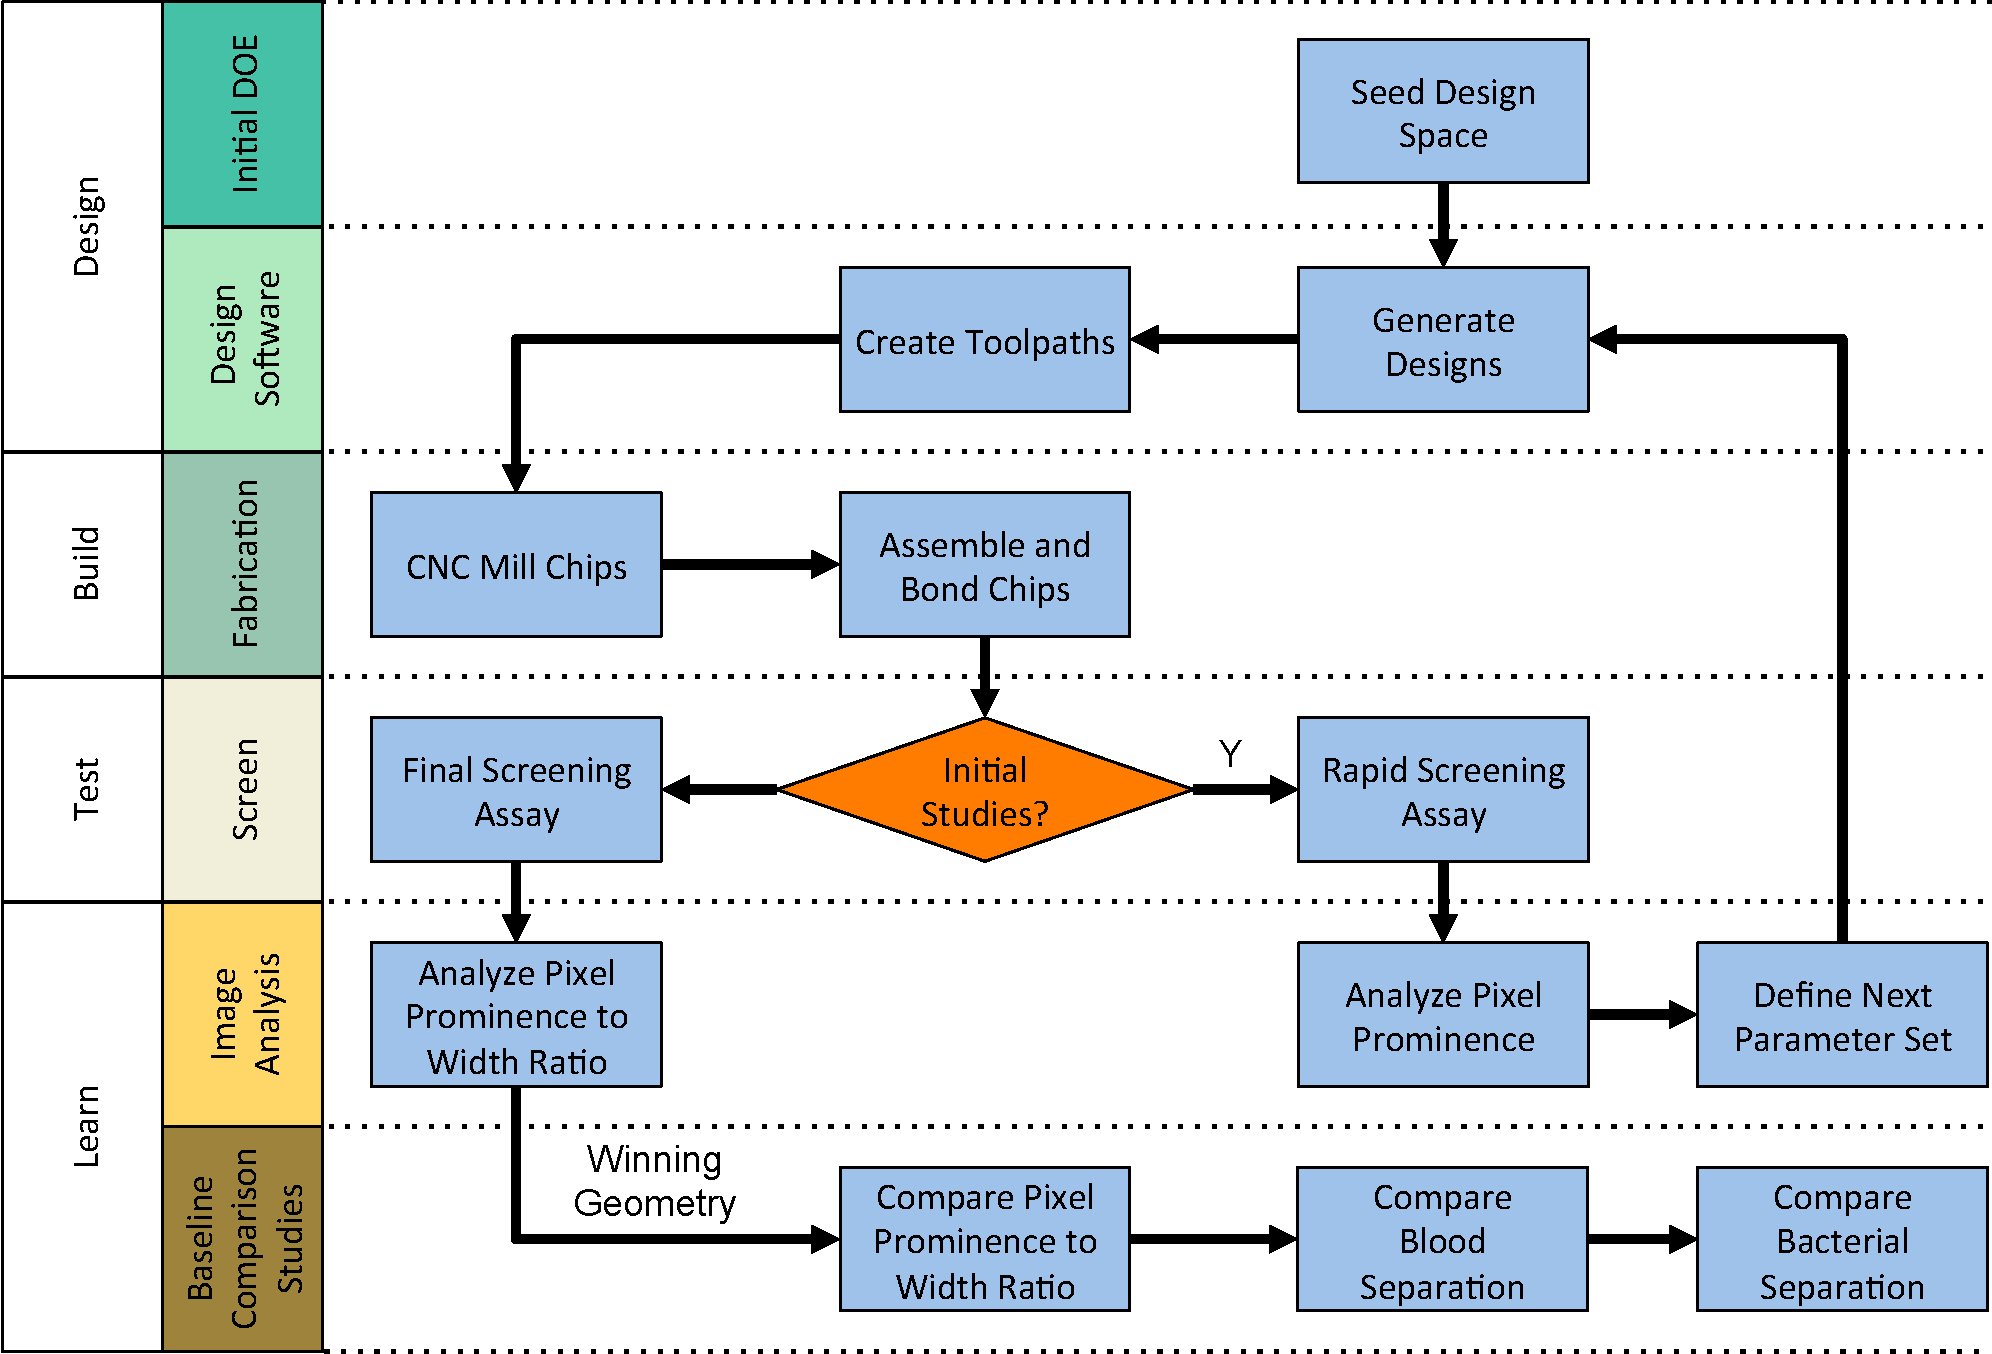
\includegraphics[width=14cm]{flow.pdf}
  \end{minipage}\hfill
  \caption[Rapid prototyping workflow]{Iterative rapid prototyping and testing workflow. The design space was first seeded using a design of experiments tool known as an orthogonal array, which minimizes the number of necessary experiments when compared to a full-factorial experimental analysis (Section \ref{ssec:seeding}). Trends were then identified within single geometric variables and experimentally explored. These variable isolation studies were repeated until a fully functional design set was achieved (Section \ref{ssec:iso}). The best performing device geometry emerging from the workflow, Chip 2.0, is then compared to the baseline using image processing, blood separation, and, finally, bacterial separation tests (Section \ref{ssec:comparison}).}
\label{fig:flow}       % Give a unique label
\end{figure}

Devices were screened in rapid succession using an image-based performance parameter of RBC acoustophoresis,  described in Section \ref{sec:img}, while varying two measures of merit: dissipated power and volumetric flow rate. As a final validation, the improved design was compared to the baseline in the task of separating bacteria from blood and shown to achieve comparable separation with significant advantages in the figures of merit. This improved device offers increased throughput and reduced power requirements and could improve performance in future point-of-care plastic acoustofluidic devices.

Figure \ref{fig:flow} illustrates the iterative workflow used in conducting the study, further described in Section \ref{sec:experiment}. Section \ref{sec:experiment} summarizes the approach used to design variable chip geometries and defines the two types of tests used in the screening phase of the workflow. Section \ref{sec:methods} outlines the methods used to screen separation performance from microscope images. Finally, Section \ref{sec:results} presents the results of the device screening as well as the winning design's performance when compared to that of the baseline geometry. 

\begin{figure}[htb]
  \begin{minipage}[t]{0.99\linewidth}\centering
    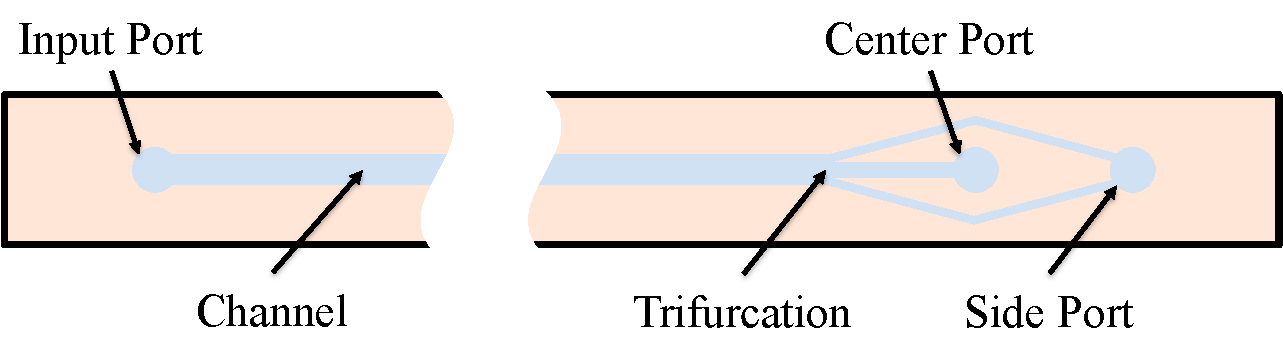
\includegraphics[width=14cm]{chip}
    \medskip
    \centerline{(a)}
  \end{minipage}\hfill\\
  \begin{minipage}[t]{0.99\linewidth}\centering
    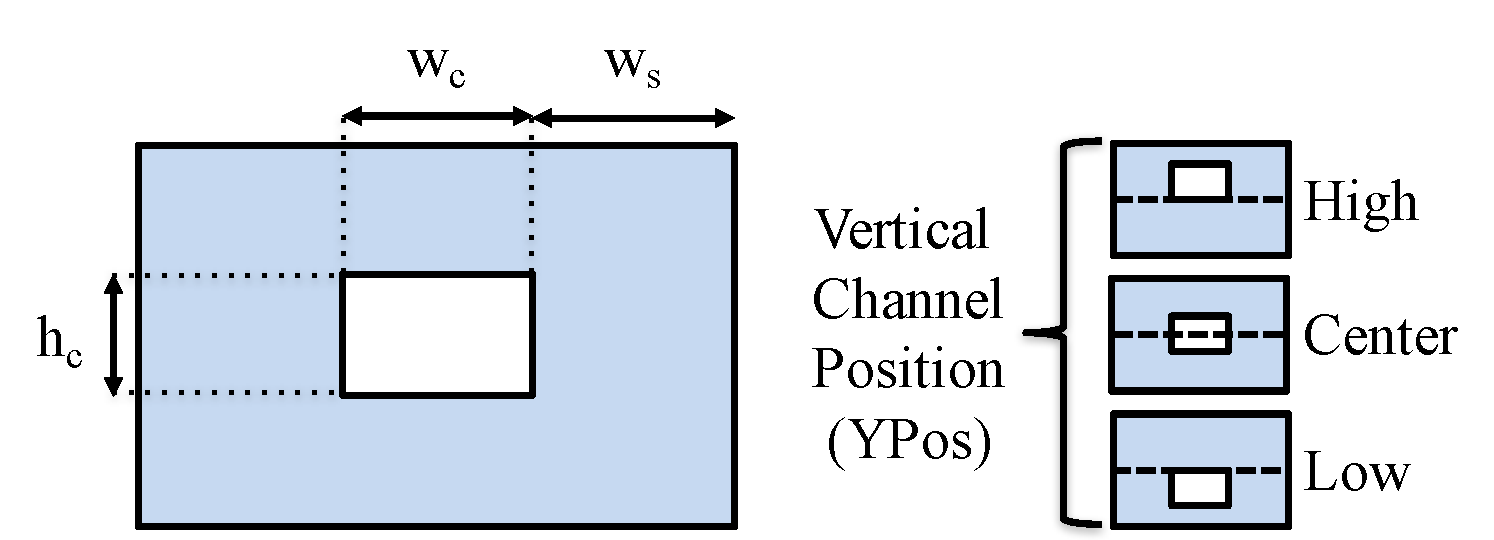
\includegraphics[width=14cm]{2D}
    \medskip
    \centerline{(b)}
  \end{minipage}
  \caption[Acoustofluidic separation device and 2D geometric definitions]{Acoustic separation device. (a) Complete trifurcated microfluidic separation chip. (b) Definitions for each two-dimensional geometry included in the study. Note that the definitions apply to the fluidic channel upstream of the trifurcation.} 
  \label{fig:geometry}
\end{figure}


Figure \ref{fig:geometry}a. is a top-down, two-dimensional drawing of the trifurcated acoustic separation device. The device functions by focusing large particles, such as RBCs and WBCs, to the center port, while smaller particles (ex., platelets, bacteria, etc.) are collected at the side port. This trifurcated device is used in the blood and bacterial separation experiments. In order to reduce manufacturing complexity, devices screened using the methods outlined in Sections \ref{sssec:rapidScreen} and \ref{sssec:finalScreen} consist only of the input port; fluid channel, defined as the channel upstream of the trifurcation; and a single output port. The cross-sectional geometries, defined in Figure \ref{fig:geometry}b., apply to this simplified device design. 

\section{Experimental Methodology}
\label{sec:experiment}

\subsection{Rapid Prototyping}
\label{sec:rp}
This study relied upon the ability to design and fabricate iterations of chip geometries in a rapid process informed by experimental tests. The traditional workflow of conventional machining requires a fully specified mechanical drawing and changes to the design may demand regeneration of the solid model and revised setup of the milling instrument.  This section describes how these limitations were mitigated using free and open-source design software in conjunction with a \$3,199 USD desktop micromill (Othermill Pro, Other Machine Co., Berkeley, CA, USA).  Microchannels with parameterized dimensions were systematically fabricated with a minimum of operator intervention.

\begin{minipage}{0.95\linewidth}
\begin{lstlisting}[caption={The custom OpenSCAD library allows solid model creation using just a single line of code},label={lst:chip}, frame=single, language=scad]
  chip(Wc=0.55,Hc=0.25,Ws=0.85,YPos=high);
\end{lstlisting}
\end{minipage}

\begin{figure}[htb]
  \begin{minipage}[t]{0.99\linewidth}\centering
    
\includegraphics[width=14cm]{PaperExampleListing1}
  \end{minipage}\hfill
  \caption[Single solid geometry]{Output solid geometry of Listing 1, including bonding plate.}
  \label{fig:listing1}
\end{figure}

\begin{minipage}{0.95\linewidth}
\begin{lstlisting}[caption={The single line of code in Listing \ref{lst:chip} can then be iterated upon to form an array of different device geometries that can be sent directly to a CAM tool for toolpath generation}, label={lst:chipLayout}, frame=single, language=scad]
include<chip.scad>

wc=[1.5,1,0.5];		 
ws=[0.5,1.5,2.5];
hc=[0.1,0.2,0.25];
ypos=[high,high,high];
Spacing=0.79375;         //End Mill Diameter

numChips=len(wc);	 //Total chips to make

module chipLayout(){
  //Iterate over number of chips
  for(i=[0:(numChips-1)]){
    let (ChipY=wc[i]+ws[i]*2){
      //Correctly space chips apart
      translate([0,2*i*(ChipY+Spacing),0])
      chip(Wc=wc[i],Hc=hc[i],Ws=ws[i],YPos=ypos[i]);
    }
  }
}
\end{lstlisting}
\end{minipage}


\begin{figure}[htb]
  \begin{minipage}[t]{0.99\linewidth}\centering
    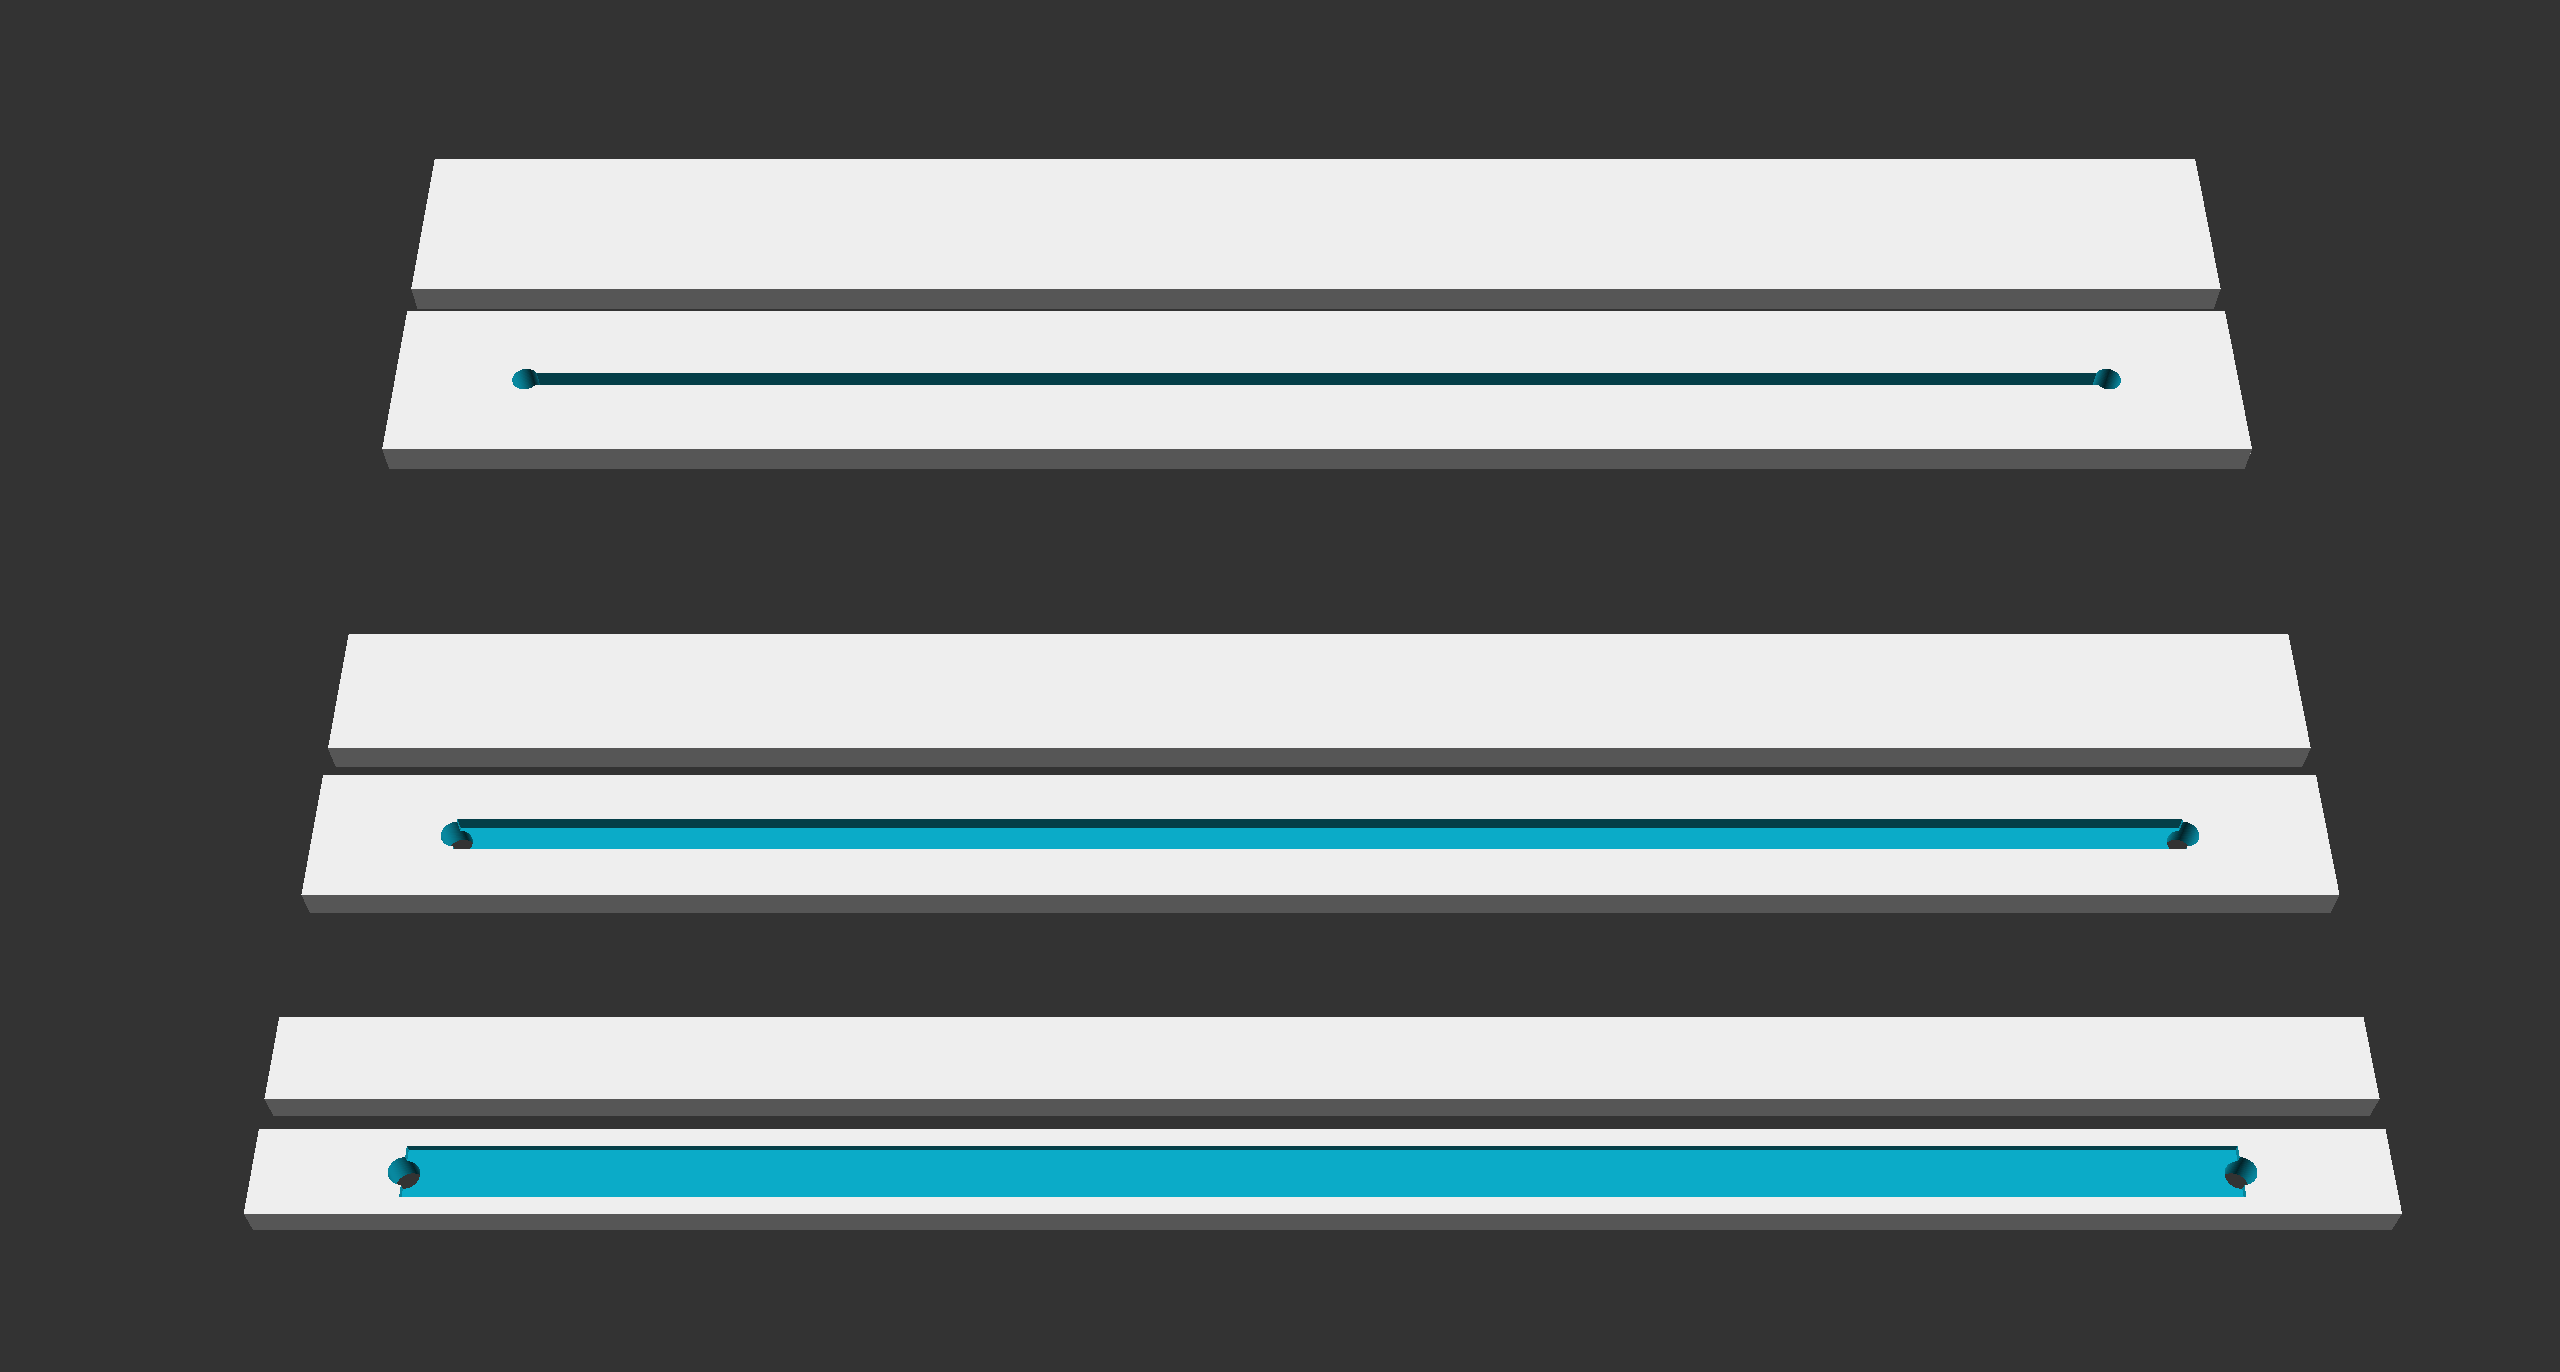
\includegraphics[width=14cm]{ExampleLayout}
  \end{minipage}\hfill
  \caption[Example layout of multiple device designs]{Output solid geometry of Listing 2, which includes three different designs and their corresponding bonding plates.}
	\label{fig:layout}
\end{figure}

\subsubsection{Design Generation}
\label{ssec:design}
Three levels of software are required to design and fabricate a novel chip geometry using a computer numerical control (CNC) micromill: a computer aided design (CAD) tool is used to create a solid model of the device; computer aided manufacturing (CAM) software generates the commands (also called toolpaths) that are sent directly to the micromill; and control software manages the connection between a computer and the micromill and sends individual toolpaths to the micromill. 

Device designs were created using OpenSCAD \cite{wikiOpenScad}, a free and open source CAD tool that reads script files to generate solid models. A custom library was used to create solid models using just the geometric parameters outlined in Figure \ref{fig:geometry}b. as inputs. Figure \ref{fig:layout} shows how an array of distinct solid models can be created from a few lines of code shown in Listing \ref{lst:chipLayout}. This array of designs is spaced according the size of the endmill used by the CNC to cut out each design, thus allowing for seamless processing by CAM software (Autodesk Fusion 360).

\subsubsection{Fabrication}
\label{ssec:fab}

Micromilling has demonstrated advantages for low-volume prototyping of plastic microfluidic devices in terms of time and cost when compared to other fabrication methods such as embossing and injection molding \cite{guckenberger2015micromilling}. While such studies claim that micromilling devices using an outside source can lower costs to \$137 per batch and 11-15 days of turn-around time, these costs only consider material costs and not labor, which can drive up the cost of prototyping an order of magnitude \cite{guckenberger2015micromilling}. Costs per device can be lowered to less than \$1 if devices can be fabricated in-house; however, the costs associated with establishing such capabilities can be prohibitive. It is only very recently that high quality micromills have been available at low cost: As recently as 2015, micromills capable of achieving resolutions at or below 25$\mu$m were available for a minimum of \$15k \cite{guckenberger2015micromilling}. The large footprints and noise associated with these machines made them inappropriate for use within a microfluidics laboratory. Additionally, the cost in terms of expertise required to operate a micromill is non-trivial. The software stack associated with generating toolpaths for a micromill does not currently resemble the simplicity of other CNC machines such as 3D printers. Traditional micromilling requires a suite of CAM tools that demand extensive knowledge of various tooling strategies such as feed rate, depth of cut and spindle speed that vary with each material and tool size. 

Recent advances in micromilling has led to the formation of a new class of desktop micromills, which can approach 25$\mu$m resolution at costs starting at \$2,500 all in a form-factor appropriate for a typical laboratory bench \cite{yen2016cost}. While these new machines still require knowledge of CAD and CAM software tools, research in automation techniques specifically for micromilling microfluidics is beginning to bear fruit \cite{silva2016iwbda}\cite{mcdaniel2017case}. This study leverages these advancements to quickly manufacture distinct acoustofluidic device designs at a negligible cost when compared to outsourcing fabrication.

\subsection{Device Evaluation}
\label{sec:eval}
We organized this study into four types of experiments: rapid screening, final screening, blood separation, and bacterial separation, progressing toward the selected design and then validating its performance in a series of functional tests. Rapid screening tests were conducted on two initial sets of designs for which the functionality of each design in the set could not be assumed, as shown in Figure \ref{fig:flow}. The methodology for this test is outlined in Section \ref{sssec:rapidScreen}. The results of these two initial rapid screening tests were then used to inform the parameter set of a final, more involved, screening test described in Section \ref{sssec:finalScreen}. Next, the winning geometry after final screening, hereafter referred to as Chip 2.0,  was compared to that of the baseline geometry in two different experiments measuring a device's ability to focus RBCs.  Finally, Chip 2.0 was compared to the baseline in experiments separating bacteria from diluted whole blood. The methodologies for each experiment are outlined in the subsections below. 

The screening tests analyzed microscope images and derived pixel intensities as an indicator of RBC focusing performance. This method assumes that higher concentrations of RBCs will appear visibly darker, and hence have a higher inverse grayscale value, when better acoustic focusing is present \cite{barnkob2012measuring}. Figures \ref{fig:pixelPerformance} and \ref{fig:microscopePics},  demonstrate that in conditions conducive to good focusing (ex., lower flow rate and higher dissipated power) the observable band of blood cells will appear narrower and darker and thus have a correspondingly higher inverse grayscale value within this band. 

\begin{figure}[htb]
  \begin{minipage}[t]{0.49\linewidth}\centering
    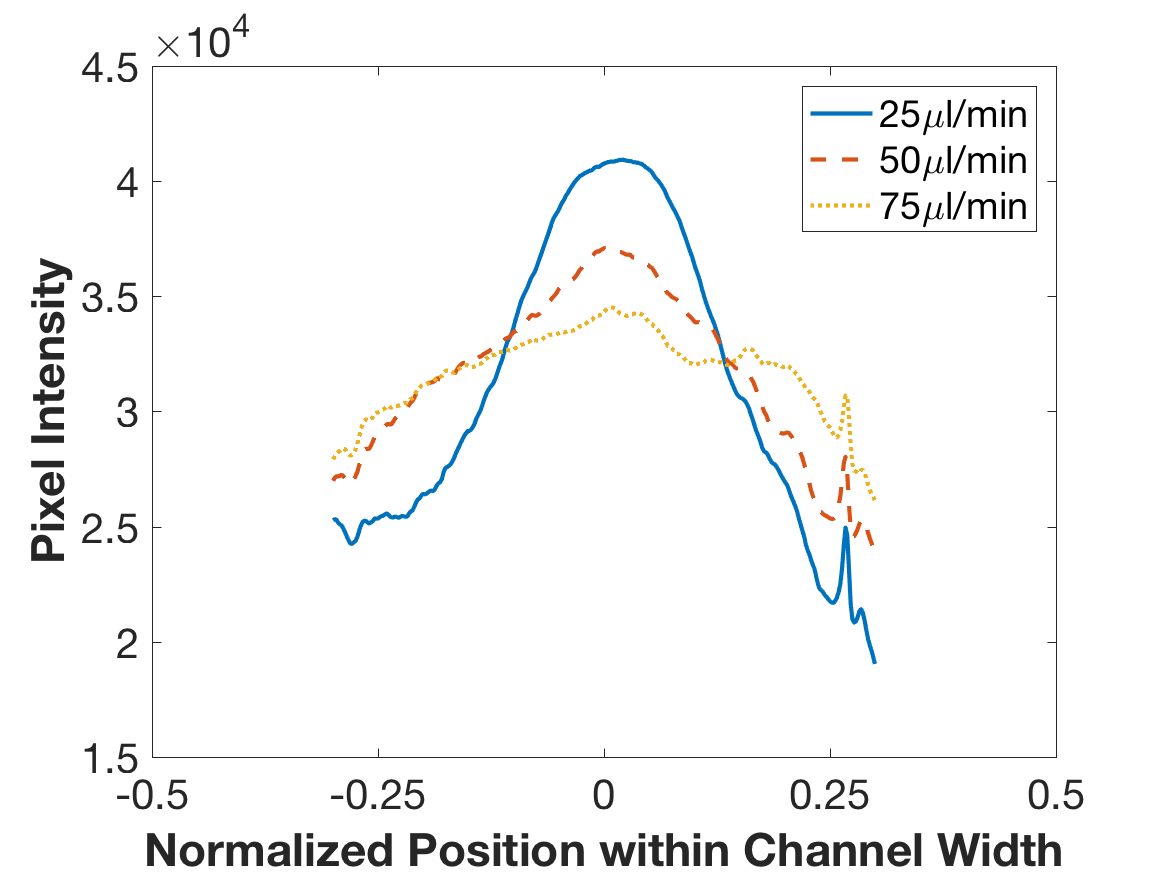
\includegraphics[width=7cm]{Baseline3PromFlow}
    \medskip
    \centerline{(a)}
  \end{minipage}\hfill
  \begin{minipage}[t]{0.49\linewidth}\centering
    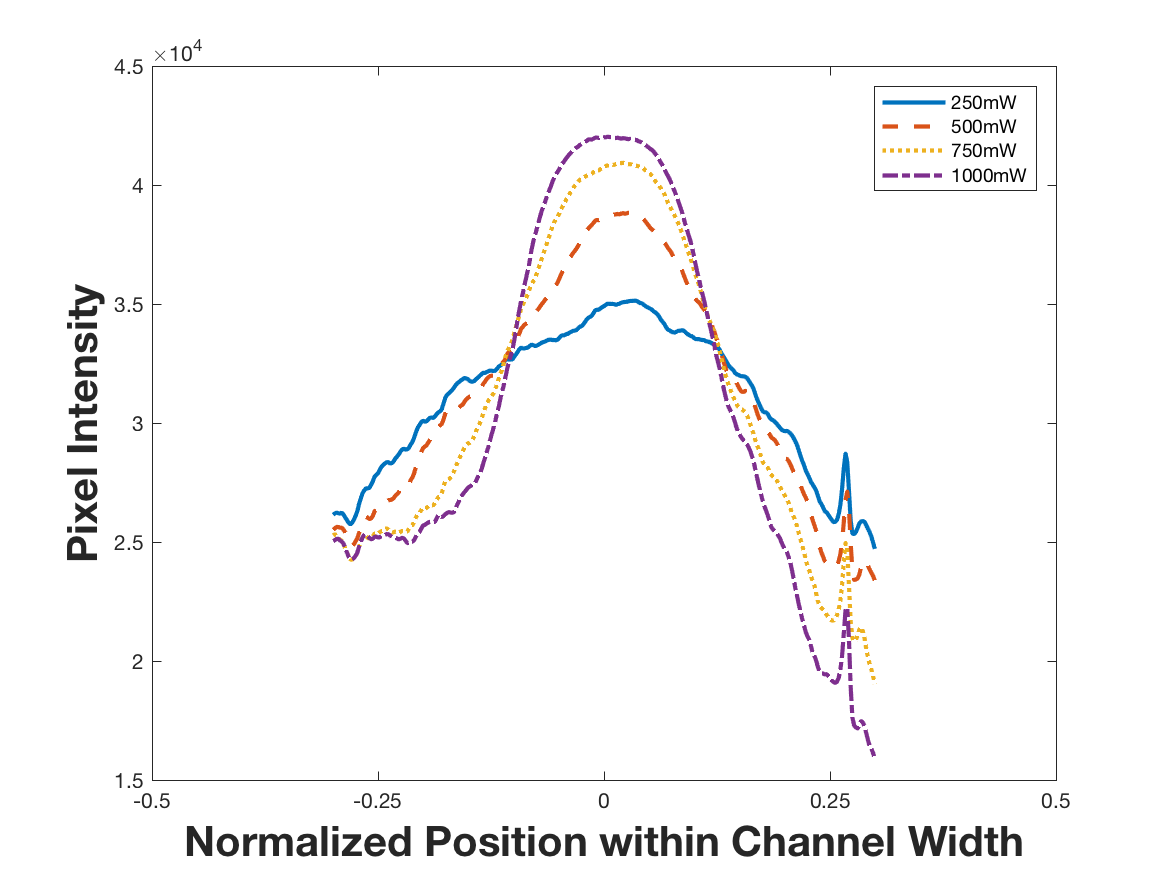
\includegraphics[width=7cm]{Baseline3PromPower}
    \medskip
    \centerline{(b)}
  \end{minipage}
  \caption[Pixel grayscale values across the width of the fluidic channel]{Pixel intensity as a surrogate for RBC focusing performance. Inverted pixel grayscale values (i.e., darker areas have a higher value) across the width of the fluidic channel. (a) Power is held constant at 750 mW while flow rate is varied. Note that maximum pixel intensity, and thus focusing performance, increases as flow rate is decreased. (b) Flow rate is held constant at 25 $\mu$l/min, while power is varied. Note that focusing performance increases as power is increased.}
	\label{fig:pixelPerformance}
\end{figure}

\begin{figure}[htb]
  \begin{minipage}[t]{0.49\linewidth}\centering
    
\includegraphics[width=7cm]{25ul250mWBaseline_3}
    \medskip
    \centerline{(a) 250mW}
  \end{minipage}\hfill
  \begin{minipage}[t]{0.49\linewidth}\centering
    
\includegraphics[width=7cm]{25ul500mWBaseline_3}
    \medskip
    \centerline{(b) 500mW}
  \end{minipage}\\
  \begin{minipage}[t]{0.49\linewidth}\centering
    
\includegraphics[width=7cm]{25ul750mWBaseline_3}
    \medskip
    \centerline{(c) 750mW}
  \end{minipage}\hfill
  \begin{minipage}[t]{0.49\linewidth}\centering
    
\includegraphics[width=7cm]{25ul1000mWBaseline_3}
    \medskip
    \centerline{(d) 1000mW}
  \end{minipage}\\
  \caption[Microscope images at resonant frequency for increasing power levels]{Microscope images of focusing performance at resonant frequency with increasing power at levels of 250mW (a), 500mW (b), 750mW (c), 1000mW (d). The plots in Figure \ref{fig:pixelPerformance}(b) are derived directly from these images.}
	\label{fig:microscopePics}
\end{figure}

The two types of screening tests, rapid screening and final screening, each have different assumptions regarding the nature of their input parameter sets. In the rapid screening test a device may not exhibit acoustic focusing at any frequency under the experimental conditions; thus, the performance parameter determines the existence of acoustic focusing, but does not discern the relative quality of focusing between devices.  In contrast, the final screening test attempts to compare the relative performance of devices that exhibit some acceptable measure of focusing performance. 

The latter separation experiments measured a device's ability to maintain cell separation performance while minimizing dissipated power to the transducer (i.e. amplitude of acoustic excitation) and maximizing sample throughput (i.e., volumetric flow rate). Maximizing the volumetric flow rate will enable the largest volume of input sample to be enriched in the shortest amount of time. Minimizing the power requirements of the system is another important measure of merit because heat generated in the transducer and in the PS channel during actuation may lead to delamination of the channel or may be harmful to the clinical sample. Therefore, it is best to drive the system at the smallest amplitude necessary to achieve acceptable performance. 

\subsubsection{Rapid Screening Test}
\label{sssec:rapidScreen}

The purpose of the rapid screening test was to discover functional device designs, i.e., designs that could focus blood, and the frequencies at which they operate. Functionality of an acoustofluidic device was determined by analyzing the strength of focusing bands whose maxima occurs within the center fifth of the channel width, as the purpose of the device is to focus RBCs into the center channel of the trifurcation shown in Figure \ref{fig:geometry}. Thus, in order to affirm the decision node labeled ``Focusing Observed Across Set'' in Figure \ref{fig:flow}, the point of maximum pixel intensity must be present in the center fifth of the channel for the device under test. 

Each set of devices was tested under the same power and flow conditions while sweeping through a frequency band  of  0.50 -- 2.00 MHz.  This range was informed by the optimum frequency of the baseline device (1.012 MHz).  The transducer was selected with a resonant frequency of 2.34 MHz to avoid confounding effects of transducer resonance. The flow rate was set such that the average velocity in each chip was  1.94 cm/sec, a value that is equivalent to 100 $\mu$l/min in the baseline device. The input power to the RF amplifier was set such that the average dissipated power at the transducer was 1 W at 1 MHz. Electrical equipment settings (ex., input voltage, RF amplifier gain, etc.) for this condition (i.e., 1 W at 1 MHz) were held constant as the frequency was varied. Within the tested bandwidth photos of the downstream end of the channel were taken in 10 kHz increments, from which a number corresponding to the maximum peak prominence was returned.   Prominence is a measure of a ``peak'' in pixel intensity and is defined further in the Methods section. The maximum peak prominence for the entire frequency band constituted the score for that particular design. An example frequency sweep is shown in Figure \ref{fig:freqSweep}.

%(\textbf{FOR JASON:} $Q=VA$; $A=0.043cm*0.02cm=0.00086cm^2$; $Q=100\mu L/min=0.1cm^3/min$; $V=\frac{Q}{A}=\frac{0.1}{0.00086}=116.3 cm/min=1.94 cm/sec$)

\begin{figure}[htb]
  \begin{minipage}[t]{0.99\linewidth}\centering
	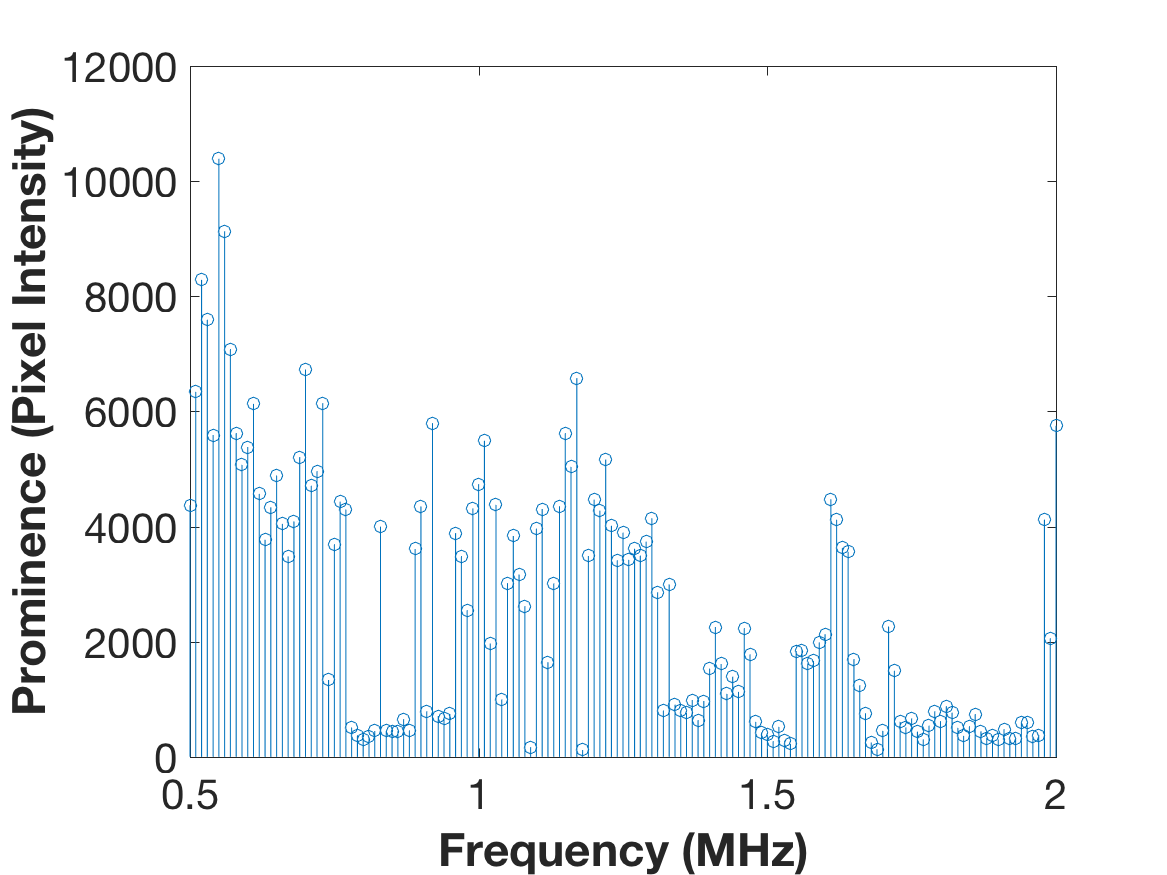
\includegraphics[width=12cm]{freqSweep}
  \end{minipage}\hfill
	\caption[Prominence versus frequency across swept bandwidth]{Prominence versus Frequency for a fixed input voltage for device 4L9 in Table \ref{tab:geometries}. Images were captured in 10 kHz increments over the bandwith extending from 0.5 MHz to 2 MHz, inclusive.}
	\label{fig:freqSweep}
\end{figure}

\subsubsection{Final Screening Test}
\label{sssec:finalScreen}

The final screening test served to discriminate between devices that exhibited RBC focusing on the rapid screening test. This was accomplished by manually tuning the device to its optimum frequency (by visual inspection of the RBC focusing) and then modulating the measures of merit. Three flow rates (25 $\mu$l/min, 50 $\mu$l/min, and 75 $\mu$l/min) and four power levels (250 mW, 500 mW, 750 mW, and 1000 mW) were studied. A microscope image was captured for each combination of flow rate and power level, from which the ratio of peak prominence to width was calculated in accordance with the method described in Section \ref{ssec:promToWidth}.  The ratio of peak prominence to width serves as a predictor of the device's ability to separate RBCs.

\subsubsection{Blood Separation Test}
\label{ssec:bloodAssay}

The purpose of the blood separation test is to measure a device's ability to focus RBCs to the center port of the device at a series of combinations of flow rate and power settings. A test of this sort has proven useful in assessing or comparing the acoustic energy density in several device configurations for applications ranging from high-throughput cell sorting \cite{adams2012high}\cite{mueller2013continuous} to plasmapheresis \cite{lenshof2009acoustic}. Samples of dilute whole blood were collected from both side and center ports for each setting according to the protocol established in Section \ref{sec:sampleMeasurement}. Performance is measured using RBC separation percentage, calculated by dividing the number of RBCs collected from the center port and dividing by the total number of RBCs collected from both outlet ports.

\subsubsection{Bacterial Separation Test}
\label{ssec:bacteriaAssay}

The goal of the bacterial separation experiments is to determine the maximum capacity of a chip design in its ability to separate bacteria from blood, as has been demonstrated in other acoustic microfluidic devices \cite{ohlsson2016integrated}\cite{li2016acoustofluidic}. The operational capacity of a chip is evaluated in terms of the two measures of merit: volumetric flow rate and average dissipated power, each tested with the other fixed.  Bacterial separation is measured at the point of minimum power or maximum flow rate required to achieve 90\% separation of RBCs, measured by the ratio of colony forming units (CFU) to RBCs present in the side port.  Where power was varied, flow rate was held at 50 $\mu$l/min.  Where flow rate was varied, power was held at 1 W. 

\section{Methods}
\label{sec:methods}

\subsection{Materials and Assembly}
Polystyrene (PS) was selected as an appropriate material based on its relatively low attenuation and high acoustic impedance relative to other plastics \cite{mueller2013continuous}\cite{selfridge1985approximate}. The chip was sealed using a thermal bonding method previously described \cite{mueller2013continuous}. 0.75'' lengths of polyetheretherketone (PEEK) tubing served as an interface between the PS chip and the longer lengths of polyvinyl chloride (PVC) tubing used to introduce and collect sample. The rigid PEEK tubing was inserted into machined port cavities and affixed to the chip using epoxy (Epoxy 907, Miller-Stephenson, Danbury, CT, USA). 

Lengths of vinyl capillary tubing  were appended to the outlet ports to divide outlet volumes at a ratio of 60\% volume measured at the side port to 40\% at the center, using relative resistances. 

%tubing length was cut to match the ratio of hydraulic diameters of each channel. Once flow fractions matched outlet dimensions, the channel was primed with deionized (DI) water, followed by the sample.  Once the sample being tested occupied the total volume of the microfluidic chip and inlet/outlet tubing, the flow rate was set to appropriate setting on the syringe pump.  Control measurements were taken for each flow rate with the acoustics off to validate flow fraction as well as cellular behavior within microfluidic chip.  Samples were collected in conical tubes and measured for flow fraction and cell quantity calculations. The resonant frequency was found visually by observing the focusing stream -- the most compact stream reveals the resonant frequency.  Once the resonant frequency was found, powers were swept by increasing RF amplifier gain to encompass the experimental parameters.  For each sample, weights and hematology data was taken and entered into a database.  MATLAB was used for further data analysis and plotting.  

The sealed chip was mounted to a lead zirconate titanate (PZT) transducer (APC International, PZT 850) with a published resonance of 2.34 MHz using low viscosity cyanoacrylate adhesive.  

\subsection{Image Processing and Analysis}
\label{sec:img}
Image processing software (ImageJ \cite{imagej}) was used to measure pixel intensities across the width of the channel, $W_c$, from which prominence was calculated. The prominence of the focused stream, as described in detail in Section \ref{ssec:prom} below, served as a measure of the degree of focusing and the performance of the chip. Prominence has advantages over raw pixel intensity for the purposes of comparison due to its self-normalizing nature. Since prominence is measured relative to points on the signal itself it is robust against irregularities inherent to the signal. These irregularities can take the form of variable lighting conditions between experimental runs, such as variations in environmental lighting, and illumination variabilities within a single microscope image's region of interest, such as skewed background intensities caused by shadows. 

%Peak prominence is used as a direct measure of merit for device rapid screening studies.  When a device is determined to function well based on its prominence score it is compared to the baseline geometry (final screening) using the ratio of peak prominence to half-prominence width, $\chi$ (Figure \ref{fig:algProg}c.). $\chi$ cannot be used during device screening as the metric can skew results by rewarding peaks with relatively small prominence values and correspondingly small widths. However, this metric is useful for comparing the quality of the most prominent peaks among different, commensurate, devices such as the winner of a design screening iteration and the baseline geometry.


\subsubsection{Definition of Prominence}
\label{ssec:prom}
Suppose an ordered signal is defined as in Equation \ref{eqn:sig}, where set $D$ consists of $N$ data points. Prominence is calculated by first finding all local maxima within the response set $D$ and then determining a reference point on the signal associated with each local maxima \cite{freeman1977corner}\cite{arge2013algorithms}. Briefly, this reference point is established by drawing a horizontal line in both the positive and negative directions from the local maxima (labeled as ``Scan High'' and ``Scan Low'', respectively, in Figure \ref{fig:algProg}) until either the end of the signal is reached (as in the case of $i_{high}$, in Figure \ref{fig:algProg}) or until the line intersects the signal itself ($i_{low}$, in Figure \ref{fig:algProg}), thus creating two sets of data points in the positive and negative directions. Minima are determined for each of the data sets, and prominence is then defined as the height of the local maxima relative to the maximum of these two established minima ($s_{ref}$). 

\begin{equation}
  \label{eqn:sig}
  \hfill s[n]=D \quad n=0,1,2,\cdots,N-1 \hfill
\end{equation}

A framework for defining prominence in a more formal terms begins by establishing the data structure for the signal of interest. Individual values are accessed by index such that $s[i]=d_i, d_i\in D$. Two discrete points $d_i \in D$ and $d_{i'} \in D$ are said to be $neighbors$ if $|i-i'| = 1$. A local maxima, hereafter called a $peak$, is a point $p$ where $d_i$ is greater than all of its neighbors, as defined in Algorithm \ref{alg:peaks}. The set of peaks $P \subset D$ consists of individual peak values $p \in P$. A peak is referenced by its index value $i$ in $D$ and the raw peak height is calculated by finding $s[i]$. The index in $D$ of peak $p$ is returned by the function $x(p)$. The height of peak $p$ is returned by the function $s[x(p)]$. Thus if $p \leftarrow d_i$, $x(p)=i$ and $s[x(p)]=d_i$. Prominence is then determined via Algorithm \ref{alg:prom}. 

%\paragraph{Paragraph headings} Use paragraph headings as needed.
%\begin{equation}
%a^2+b^2=c^2
%\end{equation}

\begin{figure}
\begin{algorithm}[H]
\DontPrintSemicolon
\SetKwFunction{AppendToP}{AppendToP}
\SetKwData{neighbors}{neighbors}
\KwData{Ordered data set $D$}
\KwResult{A list of peaks $P\subset D$}
\Begin{
$P \longleftarrow \emptyset$\;
\For{$d_i \in D$}{
    Find all $neighbors$ for $d_i \mid |i-i'|=1$
    $\AppendToP(neighbors)$
}
}
\caption{Find Peaks. Finds all local maxima in $D$ and returns them as a list of peaks $P$ as shown in Figure \ref{fig:algProg}(a). \label{alg:peaks}}
\end{algorithm}
\end{figure}

\begin{figure}
\begin{algorithm}[H]
\DontPrintSemicolon
\SetKwData{s_{low}}{s_{low}}
\SetKwFunction{AppendToWidth}{AppendToWidth}
\KwData{Ordered data set $D$ and a list of local maxima $P\subset D$}
\KwResult{A list of prominence values, $Prom$, for each local maxima, $p$}
\Begin{
$Prom \longleftarrow \emptyset$\;
  \For{$p_j \in P$}{
	\tcc{Scan Low}
	\For{$i = 0$ to $x(p_j)$}{
	  \If{$x(p_j)=0$}{
	    $i_{low}=x(p_j)$\;
	    Exit Loop\;
	  }
	  \ElseIf{$s[x(p_j)-i] \geq s[x(p_j)] \lor x(p_j)-i=0$}{
	    $i_{low}=x(p_j)-i$\;
	    Exit Loop\;
	  }
	}
	\For{$i = 0$ to $N-1$}{
	  \If{$x(p_j)=N-1$}{
	    $i_{high}=x(p_j)$\;
	    Exit Loop\;
	  }
	  \ElseIf{$s[x(p_j)+i] \geq s[x(p_j)] \lor x(p_j)+i=N-1$}{
	    $i_{high}=x(p_j)+i$\;
	    Exit Loop\;
	  }
	}
  $s_{low}=min(s[i_{low}] \to s[x(p_j)])$\;
  $s_{high}=min(s[x(p_j)] \to s[i_{high}])$\;
  $s_{ref}=max(s_{low},s_{high})$\;
  $Prom_j = s[x(p_j)] - s_{ref}$\;
  $\AppendToWidth(Prom_j)$\;
  }
}
\caption{\label{alg:prom}Calculate Prominence. Draw a horizontal line to the left (low) and right (high) of the peak until the end of the signal is reached or until the signal is intersected. Record the indices of each as $i_{low}$ and $i_{high}$, respectively. Find the minima in each set and use the maximum of the minima to set the reference level. Calculate a peak's prominence by subtracting the reference level from the raw signal value of the peak (Figure \ref{fig:algProg}(b-c))}
\end{algorithm}
\end{figure}

\subsection{Definition of Prominence to Width Ratio, $\chi$}
\label{ssec:promToWidth}
The half-prominence width of a peak of prominence $Prom$ is calculated by drawing two horizontal lines extending in the negative and positive directions from the point of half-prominence. These lines extend in either direction until either the end of the signal is reached or the line intersects the signal itself. The indices of these events in the negative and positive directions are recorded as $i^-$ and $i^+$, respectively. The peak width $HalfPromWidth$ is then defined as $|i^+-i^-|$, as described in Algorithm \ref{alg:width}. We reason that for equivalent separation performance, assuming a fixed ratio of flow to side and center ports \cite{ley2016continuum}, that the prominence half width scales with the channel width, therefore it is appropriate to normalize the peak width by the width of the channel. The final equation for $\chi$ is shown in Equation \ref{eqn:ratio}

\begin{figure}
\begin{algorithm}[H]
\DontPrintSemicolon
\SetKwData{s_{low}}{s_{low}}
\SetKwFunction{FindPeaks}{FindPeaks}
\KwData{A list of prominence values, $Prom$, for each local maxima, $p$}
\KwResult{A list of half-prominence peak widths $HalfPromWidth$, for each local maxima, $p$}
\Begin{
$Prom \longleftarrow \emptyset$\;
  \For{$p_k \in P$}{
	\tcc{Scan Left}
	\For{$i = 0$ to $x(p_k)$}{
	  \If{$x(p_k)=0$}{
	    $i^-=x(p_k)$\;
	    Exit Loop\;
	  }
	  \ElseIf{$s[x(p_k)-i] \leq s[x(p_k)]-\frac{Prom_k}{2} \lor x(p_k)-i=0$}{
	    $i^-=x(p_k)-i$\;
	    Exit Loop\;
	  }
	}
	\tcc{Scan Right}
	\For{$i = 0$ to $N-1$}{
	  \If{$x(p_k)=N-1$}{
	    $i^+=x(p_k)$\;
	    Exit Loop\;
	  }
	  \ElseIf{$s[x(p_k)+i] \leq s[x(p_k)]-\frac{Prom_k}{2} \lor x(p_k)+i=N-1$}{
	    $i^+=x(p_k)+i$\;
	    Exit Loop\;
	  }
	}
  $HalfPromWidth_k = i^+-i^-$\;
  $\AppendToWidth(HalfPromWidth_k)$\;
  }
}
\caption{\label{alg:width}Calculate Peak Width at Half Prominence. Draw a horizontal line to the left (-) and right (+) at the median of the prominence line until either the end of the signal is reached or until the signal is intersected. Record the indices of each as $i^{-}$ and $i^{+}$, respectively. The absolute value of the difference between these index values is the peak width at half prominence. \ref{fig:algProg}(d))}
\end{algorithm}
\end{figure}

\begin{equation}
\label{eqn:ratio}
\hfill \chi=Prom*\frac{W_c}{HalfPromWidth}\hfill
\end{equation}


\begin{figure}[htb]
  \begin{minipage}[t]{0.99\linewidth}\centering
	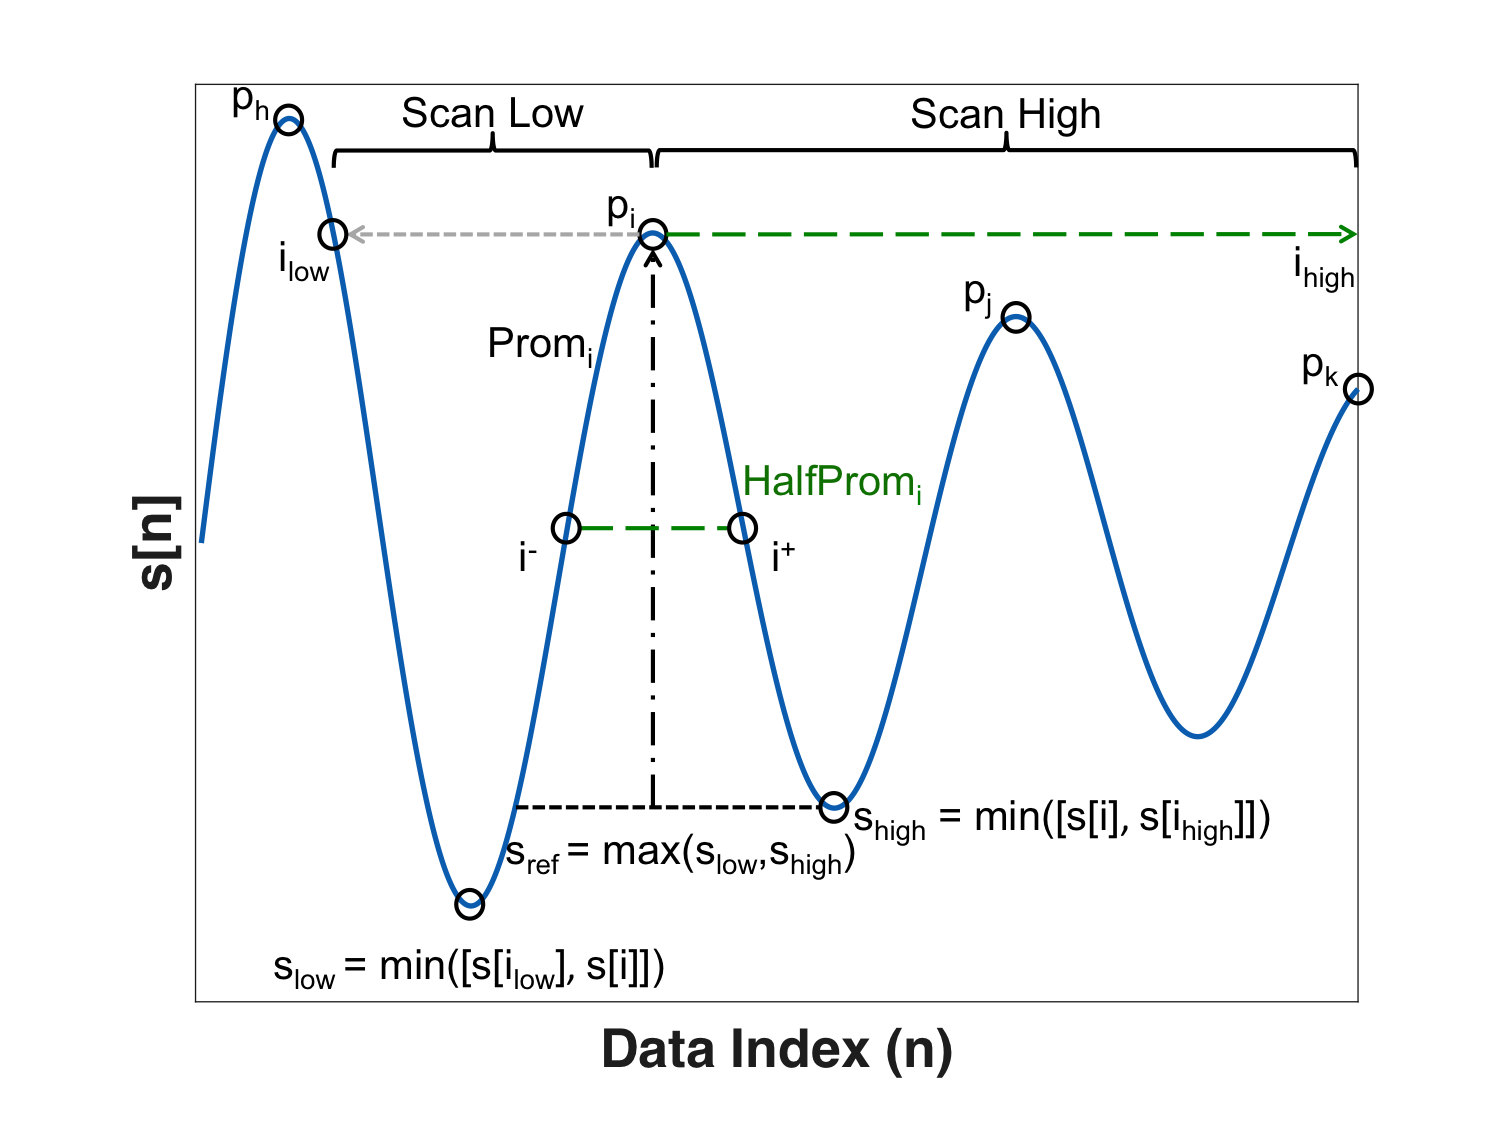
\includegraphics[width=12cm]{alg}
  \end{minipage}\hfill
  \caption[Algorithmic progression for calculating prominence]{Algorithmic progression. The blue, solid line represents a signal, $s[n]$, sampled at points, $n$, along the x-axis. Local maxima are labeled as points $p_{\{h,i,j,k\}}$. $s_{ref}$ marks the reference point from which the prominence, $Prom$, of peak $p_i$ is calculated. The width of the signal at the point of half-prominence, $HalfPromWidth$, is calculated by subtracting $i^-$ from $i^+$.}
	\label{fig:algProg}
\end{figure}

\subsection{Transducer Drive}
\label{ssec:MoM}

%The two measures of merit used in this study are average dissipated power of the transducer and volumetric flow rate of a clinical sample. Minimizing the transducer's power requirement via a geometry with an optimized resonance profile is desirable as high power requirements can result in localized heat buildup and chip failure. Maximizing volumetric flow rate allows for more rapid sample enrichment.

%\textbf{TODO Charlie: Add verbiage as to why we use Power as a measure of merit (tie displacement to power)}

The sinusoidal signal used to drive the transducer is generated by a function generator (AFG3022C, Tektronix, Beaverton, OR, USA) and amplified using a broadband RF amplifier (AG1021, T\&C Power Conversion, Rochester, NY, USA). The instantaneous voltage and current across the transducer is monitored using an oscilloscope (DPO2024B, Tektronix, Beaverton, OR, USA). In order to determine the actual power consumed by the transducer, it is first necessary to consider the instantaneous power as follows:

\begin{equation}
\label{eqn:instpower}
\hfill P_{inst} = VI = V_{max}sin(\omega t) I_{max} sin(\omega t-\varphi),\hfill
\end{equation}

\noindent where $V_{max}$ and $I_{max}$ are the maximum values of voltage and current, $\varphi$ is the phase lag between the instantaneous current and voltage signals, and $\omega=2\pi f$ is the sinusoidal drive frequency in rad/s. Using trigonometric identities and integrating over a cycle of the sinusoid we compute the average consumed power as:

\begin{equation}
\label{eqn:avgpower}
\hfill P_{avg} = V_{rms}I_{rms}cos\varphi,\hfill
\end{equation}

\noindent where $V_{rms}$ and $I_{rms}$ are the root mean square values of voltage and current. Using the oscilloscope, we multiply the instantaneous voltage and current and compute the average of this product to find the average consumed power in real time throughout our experiments.

Voltages and currents used to achieve 1 W of dissipated power at resonant frequencies for the baseline geometry and Chip 2.0 are shown in Table \ref{tab:comparison}. Note that the drive is not optimized for impedance matching, therefore most power is reflected.
\subsection{Blood Sample Preparation}
All experiments in this study used de-identified fresh human whole blood purchased from a vendor (Research Blood Components, Brighton MA), anticoagulated with acid–citrate–dextrose. In each case, the blood was diluted to 5\% by volume (for rapid screening tests) or 5\% hematocrit (for all other tests) in phosphate buffer solution (PBS 7.4 pH Lot Number 1832496). Cellular concentrations were measured before and after dilution using an automated hematology analyzer (XP-300, Sysmex Co., Kobe, Japan). The diluted sample was then transferred to a 10 ml plastic syringe (BD 10 ml Luer-Lok tip syringe 309604) and introduced to the chip through PVC tubing. The volumetric flow rate was regulated by a syringe pump (PhD Ultra, Harvard Apparatus).

\subsection{Bacteria--Blood Sample Preparation}

\textit{Pseudomonas aerouginosa}  was incubated overnight in a Lysogeny Broth (LB) culture. It was diluted by a factor of 50 and incubated until it reached a mid log phase. A whole blood sample was diluted into PBS as described in Section \ref{ssec:bloodAssay}. The optical density of the \textit{Pseudomonas} culture was taken and the appropriate dilution was calculated to create solution consisting of whole blood diluted in PBS to 5\% hematocrit and $10^5$ \textit{Pseudomonas} cells/ml. 

\subsection{Sample Measurement}
\label{sec:sampleMeasurement}

Blood or blood bacteria solutions were pumped through the device at its previously determined resonant frequency.  For each device this was found visually by observing the focusing stream--the most compact stream reveals the resonant frequency.  Outlet samples were collected in conical tubes after which they were measured and weighed for flow fraction and cell quantity calculations. 

Blood content was measured via a hematology analyzer while bacterial content was measured through a plating analysis: the samples were weighed, then serially diluted in 10x steps into PBS. Each dilution was cultured onto a plate of LB agar and incubated at 37$^{\circ}$C overnight after which the CFU were counted.   

The setpoint for 90\% RBC separation for variable power and fixed flow (50 $\mu$l/min) rate was accomplished by increasing power in small increments. Samples were collected from each output port and RBC counts were measured after each power increment. This process was repeated until a 90\% RBC separation ratio was achieved between the side and center ports.
%; smaller power increments were used to provide better resolution in determining the power conditions resulting in a separation ratio of 90\%. 

Determining 90\% RBC separation for variable flow rate and fixed power (1 W) required that the flow rate be set to 25 $\mu$l/min and increased in increments until such a point as 90\% RBC separation was achieved.  

\section{Results}
\label{sec:results}
\subsection{Screening Design of Experiments}
\label{ssec:doe}
Experiments must be initialized such that the sampling of the solution space can detect curvature in the response, as described in Section \ref{ssec:seeding}. Curvature in the response surface for an explanatory variable implies the existence of a local maxima in performance. Driving the design towards that local maxima is accomplished by isolating the variable in question and conducting experiments at adjacent points on the response plane, as outlined in Section \ref{ssec:iso}. 

Figure \ref{fig:geometry} illustrates the explanatory variables studied. Channel Width ($W_c$), channel height ($H_c$), side-wall width ($W_s$) and the position of the channel on the $y$-axis in two dimensional space ($Y_{pos}$) were selected as variables to study because they account for a majority of the two-dimensional design-space and are simple to vary during fabrication.

\subsection{Seeding of the Design Space (Rapid Screening Test)}
\label{ssec:seeding}

\begin{figure}[htb]
  \begin{minipage}[t]{0.99\linewidth}\centering
    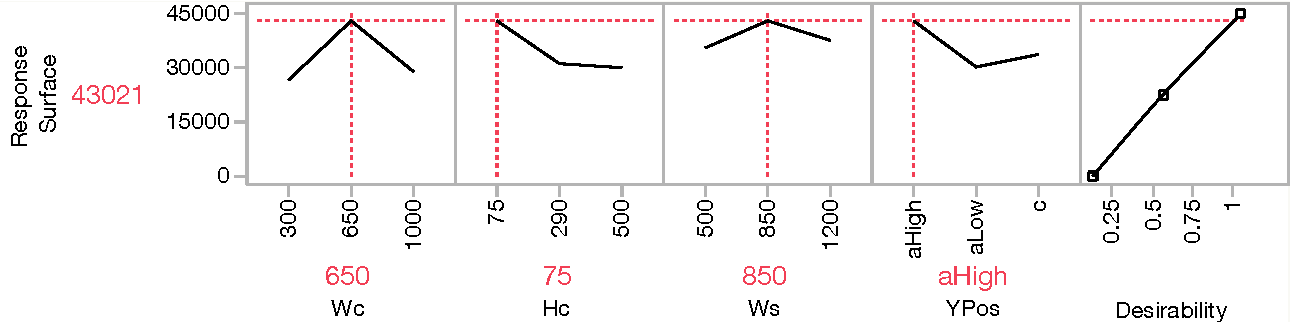
\includegraphics[width=14cm]{L9}
  \end{minipage}\hfill
  \caption[Results of initial seeding of design space]{Results of design space seeding. The quantities on the vertical axis correspond to the prominence data shown in Table \ref{tab:geometries}. The response surface is determined through a least squares fit of the aforementioned prominence values in four-dimensional space. The red dashed lines demarcate the points of maximum desirability.}
	\label{fig:L9}
\end{figure}

In order to economize the number of rapid screening experimental runs, an orthogonal array was chosen to generate a useful parameter set for the initial experiments. Orthogonal arrays are are used in design optimization to provide the most coverage of the solution space while minimizing the number of experimental runs \cite{yokoyama1993taguchi}. This is accomplished through the creation of an experimental set such that each combination of the array's strength appears equally often \cite{hedayat2012orthogonal}. The orthogonal array used to seed the design space is known as the $L_9 (3^4)$ array, which has a strength of two and is used to probe a solution space consisting of four explanatory variables at three settings in nine experimental runs, as opposed to the 81 experimental runs required to conduct the full-factorial experiment \cite{hedayat2012orthogonal}. The use of three explanatory variable settings was chosen in order to detect curvature in the response surface. The parameter set tested while seeding the design space, in accordance with an $L_9 (3^4)$ orthogonal array, is shown in Table \ref{tab:geometries}.

%Since the parameters generated during the initial seeding of the design space cannot assume a functional geometry (i.e., a geometry capable of focusing blood), the purpose of the initial iteration of experiments is directed towards discovering functional designs, as opposed to a comparison between functional designs. As such, the performance parameter used during this initial phase is peak prominence (Figure \ref{fig:algProg}c.). This is because $\chi$ (Figure \ref{fig:algProg}d.) can skew the results by rewarding peaks with small prominence values (i.e., poor focusing) and correspondingly small widths.  

\begin{table}[h]
% table caption is above the table
\caption[Geometries tested for L9 design array]{Geometries tested for L9 design array with corresponding Chip ID. All dimensions are given in units of $\mu$m. Prominence values are given in units of pixel intensity and correspond to each chip's maximum prominence value for the tested bandwidth. The given frequencies indicate the point at which the maximum prominence was observed.}
\label{tab:geometries}       % Give a unique label
% For LaTeX tables use
\centering
\begin{tabular}{lllll|cc}
\hline\noalign{\smallskip}
ID & $W_c$ & $H_c$ & $W_s$ & $Y_{Pos}$ & Prominence & $f$ ($MHz$) \\
\noalign{\smallskip}\hline\noalign{\smallskip}
1L9 & 300 & 75 & 500 & Low & 6375 & 1.58\\
2L9 & 300 & 290 & 850 & Center & 5496 & 1.22\\
3L9 & 300 & 500 & 1200 & High & 8240 & 0.67\\
4L9 & 650 & 75 & 850 & High & 43021 & 0.55\\
5L9 & 650 & 290 & 1200 & Low & 12950 & 0.66\\
6L9 & 650 & 500 & 500 & Center & 13251 & 0.57\\
7L9 & 1000 & 75 & 1200 & Center & 14215 & 0.74\\
8L9 & 1000 & 290 & 500 & High & 9574 & 0.73\\
9L9 & 1000 & 500 & 850 & Low & 3144 & 0.71\\
\noalign{\smallskip}\hline
\end{tabular}
\end{table}

The response surface generated from the data points shown in Table \ref{tab:geometries} was analyzed using statistical software (JMP®, Version 13.0.0. SAS Institute Inc., Cary, NC, 1989-2017) and is shown in Figure \ref{fig:L9}. Maximum desirability of the performance parameter (prominence) is achieved by setting $W_c$ to 650$\mu$m, $H_c$ to 75$\mu$m, $W_s$ to 850$\mu$m and placing the channel in the high vertical position (i.e., Chip 4L9 in Table \ref{tab:geometries}). Additionally, the response surface shows significant curvature while modulating the width of the channel, leading into the next iteration of the study outlined in Section \ref{sssec:width}.

\subsection{Variable Isolation Studies}
\label{ssec:iso}

\subsubsection{Channel Width Study (Rapid Screening Test)}
\label{sssec:width}

Proceeding from the  results of the initial seeding of the design space,  we fixed the other parameters from the best geometry (4L9) and varied the channel width in 50$\mu$m increments.  Although the response surface indicates that thinner channel height may be preferable,  we selected a height of 100$\mu$m for this variable isolation study, anticipating that a slightly greater channel height would have practical advantages. 

\begin{table}[h]
% table caption is above the table
	\caption[Geometries tested for an isolation study of channel width]{Geometries tested for an isolation study of channel width with corresponding Chip ID. All dimensions are given in units of $\mu$m. Prominence values are given in units of pixel intensity and correspond to each chip's maximum prominence value for the tested bandwidth. The given frequencies indicate the point at which the maximum prominence was observed. The frequency range scanned spanned from 500 kHz to 2 MHz. No focusing was observed within this range for the design with a channel width of 700$\mu$m. }   
\label{tab:width}       % Give a unique label
% For LaTeX tables use
\centering
\begin{tabular}{lllll|cc}
\hline\noalign{\smallskip}
ID & $W_c$ & $H_c$ & $W_s$ & $Y_{Pos}$ & Prominence & $f$ ($MHz$)\\
\noalign{\smallskip}\hline\noalign{\smallskip}
1Wc & 500 & 100 & 850 & High & 12143 & 0.64\\
2Wc & 550 & 100 & 850 & High & 15200 & 0.51\\
3Wc & 600 & 100 & 850 & High & 4770 & 1.58\\
4Wc & 650 & 100 & 850 & High & 5470 & 1.99\\
5Wc & 700 & 100 & 850 & High & - & - \\
\noalign{\smallskip}\hline
\end{tabular}
\end{table}

As shown in Table \ref{tab:width}, the highest performing channel width, holding other factors constant, was 550$\mu$m. Channels having a width of 600$\mu$m and above demonstrated the ability to focus RBCs to the center fifth of the channel, however the focusing was a result of driving the chip at a higher order mode thus creating more than one focusing band across the channel width. 

As a significant performance shift was observed as a result of a small adjustment to $H_c$, channel height was chosen as the variable to isolate for the next design set. 

\subsubsection{Channel Height Study (Final Screening Test)}
\label{sssec:height}

This design set fixed values for $W_c$, $W_s$, and $Y_{Pos}$ while varying $H_c$ resulting in the geometries shown in Table \ref{tab:height}. All devices in this set demonstrated focusing of blood; the frequencies for which are shown in Table \ref{tab:height}. This study was conducted in accordance with the final screening test specified in Section \ref{sssec:finalScreen}. The results shown in Figure \ref{fig:heightPlot} demonstrate that, for flow rates higher than 25 $\mu$l/min, the chip with a channel height of 250$\mu$m performed better than the other chips tested in terms of $\chi$ at all studied power levels. Thus the winning geometry of the study's device screening stage has a channel width of 550$\mu$m, a channel height of 250$\mu$m, a side-wall width of 850$\mu$m, with the channel in the High vertical position (i.e., Chip 4Hc in Table \ref{tab:height}).

\begin{figure}[H]
  \begin{minipage}[t]{0.49\linewidth}\centering
    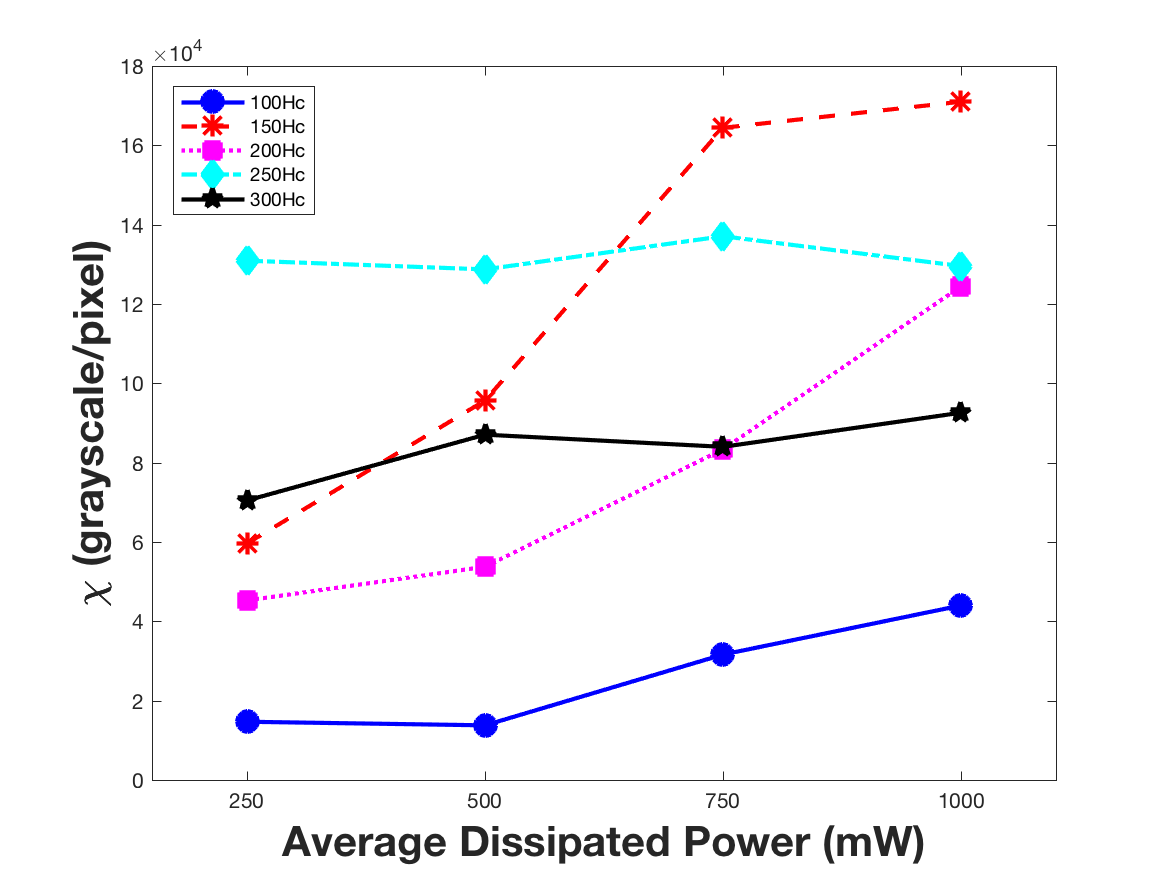
\includegraphics[width=7cm]{HeightPlot25ul}
    \medskip
    \centerline{(a) 25 $\mu$l/min}
  \end{minipage}\hfill
  \begin{minipage}[t]{0.49\linewidth}\centering
    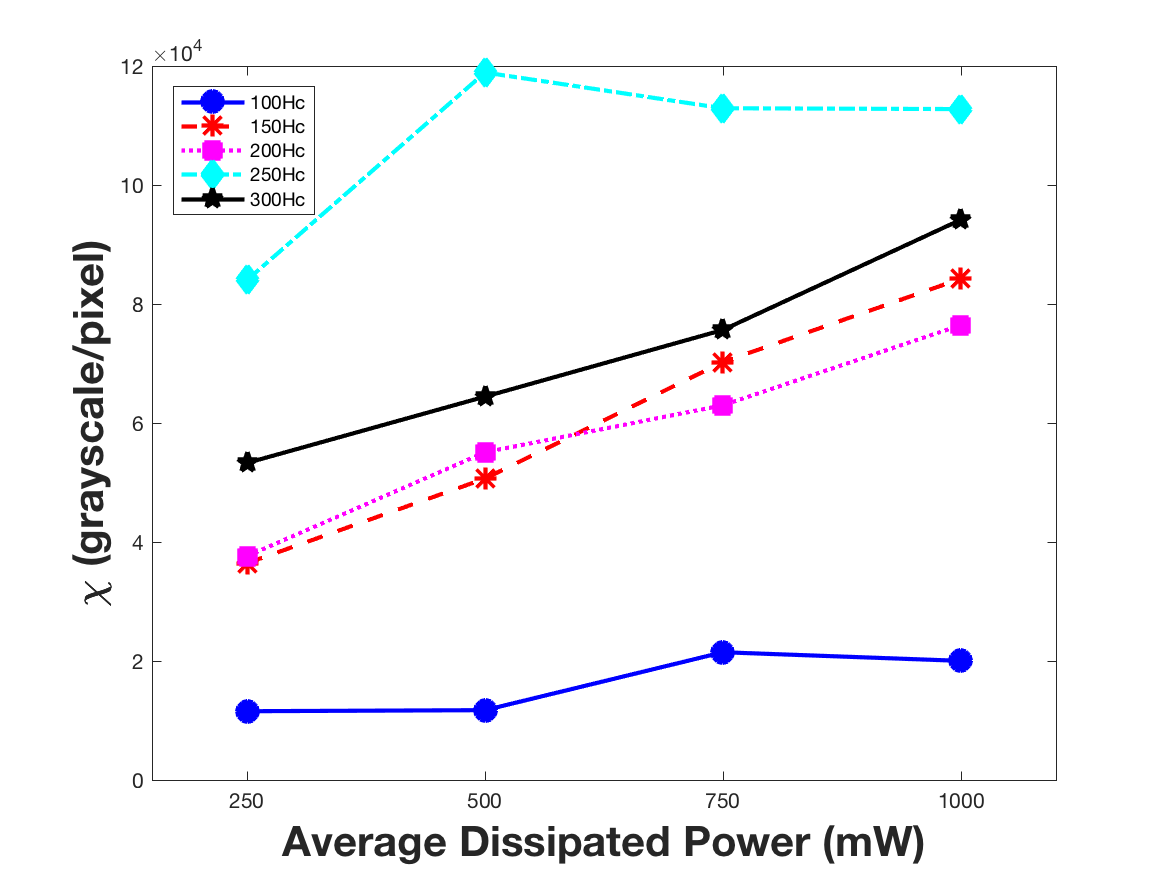
\includegraphics[width=7cm]{HeightPlot50ul}
    \medskip
    \centerline{(b) 50 $\mu$l/min}
  \end{minipage}
  \begin{minipage}[t]{0.99\linewidth}\centering
    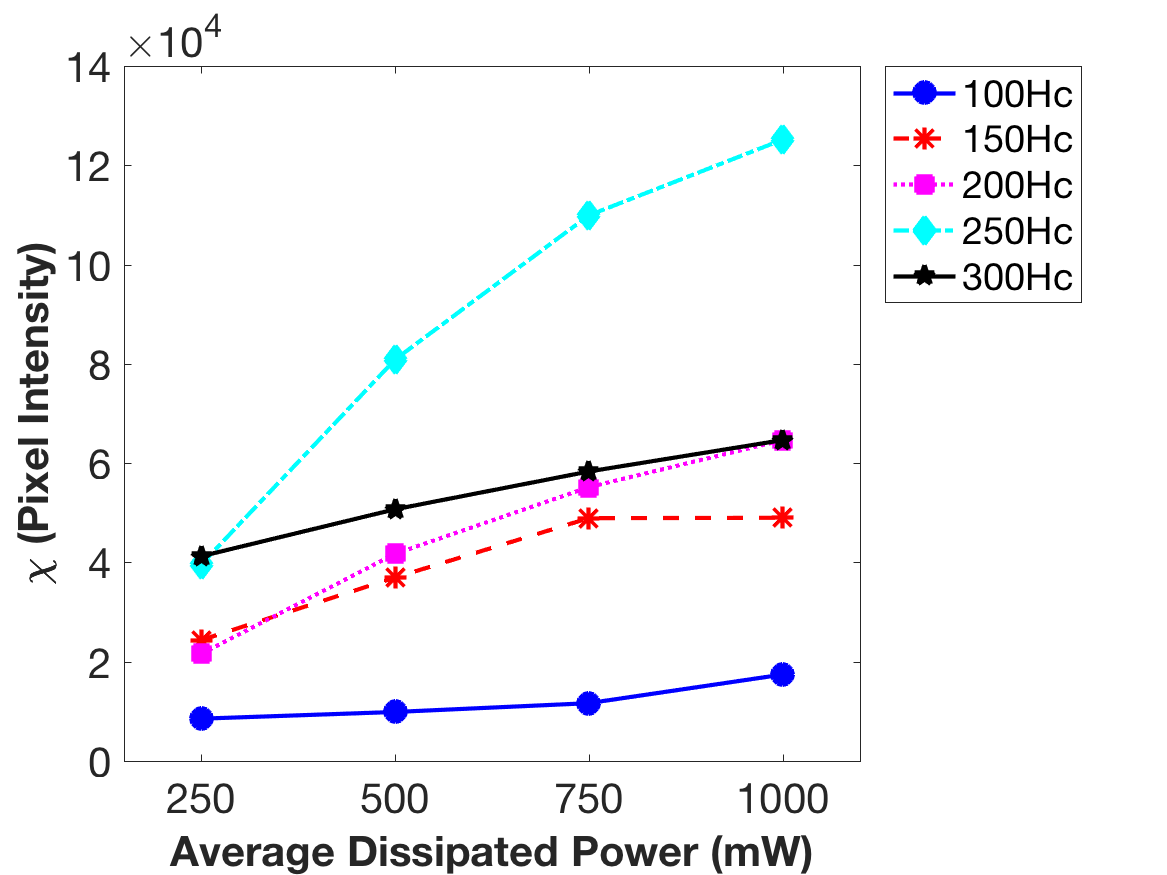
\includegraphics[width=7cm]{HeightPlot75ul}
    \medskip
    \centerline{(c) 75 $\mu$l/min}
  \end{minipage}
  \caption[Performance comparison of channel height study using image analysis]{Performance comparison of channel height study using image analysis. (a-c) plot the performance of the geometries in Table \ref{tab:height} for three volumetric flow rates: 25 $\mu$l/min, 50 $\mu$l/min and 75 $\mu$l/min, respectively. Performance is calculated from microscope images in the manner described in Section \ref{ssec:promToWidth}.  Datasets are shown for each channel height from 100 to 300$\mu$m.}
	\label{fig:heightPlot}
\end{figure}



\begin{table}[h]
% table caption is above the table
\caption[Geometries tested for a final screening study of channel height]{Geometries tested for a final screening study of channel height with corresponding Chip ID. All dimensions are given in units of $\mu$m. The listed frequencies coincide with the locations of the corresponding device's fundamental odd resonant mode.}
\label{tab:height}       % Give a unique label
% For LaTeX tables use
\centering
\begin{tabular}{lllll | c}
\hline\noalign{\smallskip}
ID & $W_c$ & $H_c$ & $W_s$ & $Y_{Pos}$ & $f$ ($MHz$)\\
\noalign{\smallskip}\hline\noalign{\smallskip}
1Hc & 550 & 100 & 850 & High & 0.684 \\
2Hc & 550 & 150 & 850 & High & 0.640 \\
3Hc & 550 & 200 & 850 & High & 0.634 \\
4Hc & 550 & 250 & 850 & High & 0.632 \\
5Hc & 550 & 300 & 850 & High & 0.640 \\
\noalign{\smallskip}\hline
\end{tabular}
\end{table}

\subsection{Comparison of Chip 2.0 versus Baseline Geometry}
\label{ssec:comparison}

The results of the screening tests shown in Figure \ref{fig:heightPlot} yield a geometry that outperformed the other devices in terms of RBC focusing analyzed by image analysis. However, in order to gauge the ultimate success of this geometry it was tested against the baseline geometry. This section presents results from three experiments that compared the winning geometry of the screening tests (i.e., Chip 2.0) against the baseline geometry through image analysis, blood separation, and bacteria separation.

\begin{table}[t]
% table caption is above the table
	\caption[Standard operating conditions for Baseline versus Chip 2.0]{Baseline versus Chip 2.0. All dimensions are given in units of $\mu$m. Standard operating conditions, measured at the transducer, are provided for frequencies, input voltages and currents required to achieve 1 W of average dissipated power. These conditions are the values for which the fundamental resonant odd modes for each chip were achieved.}
\label{tab:comparison}       % Give a unique label
% For LaTeX tables use
\centering
\begin{tabular}{lllll | ccc}
\hline\noalign{\smallskip}
Chip & $W_c$ & $H_c$ & $W_s$ & $Y_{Pos}$ & $f$ ($MHz$) & Voltage ($V_{pp}$) & Current ($mA_{pp}$) \\
\noalign{\smallskip}\hline\noalign{\smallskip}
Chip 2.0 & 550 & 250 & 850 & High & 0.632 & 56.44 ($\pm$2.4) & 1039 ($\pm$53)\\
Baseline & 430 & 200 &  1055 & High & 1.012 & 45.78 ($\pm$1.86)& 1340 ($\pm$70)\\ 
\noalign{\smallskip}\hline
\end{tabular}
\end{table}

\subsubsection{Comparative Focusing}
\label{sssec:comparisonFocusing}

\begin{figure}[H]
  \begin{minipage}[t]{0.49\linewidth}\centering
    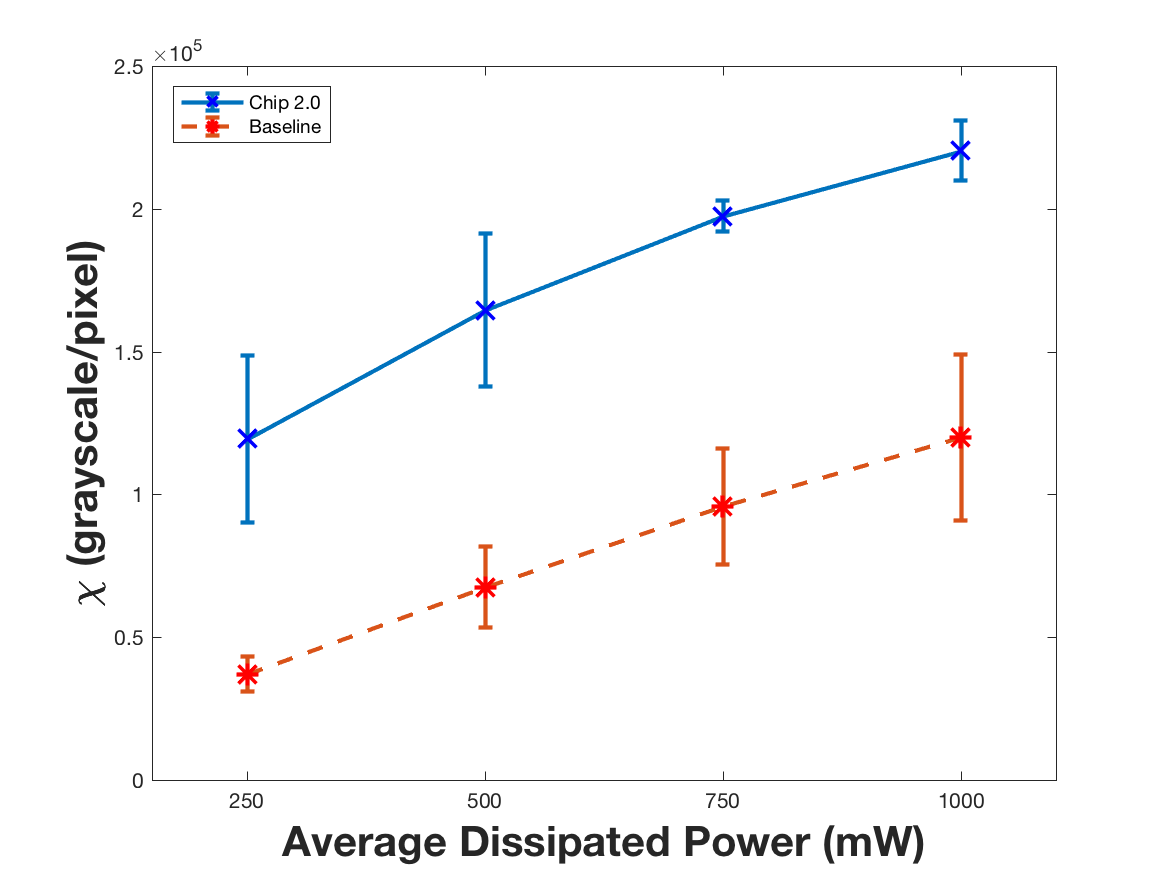
\includegraphics[width=7cm]{ErrorBars25ul}
    \medskip
    \centerline{(a) 25 $\mu$l/min}
  \end{minipage}\hfill
  \begin{minipage}[t]{0.49\linewidth}\centering
    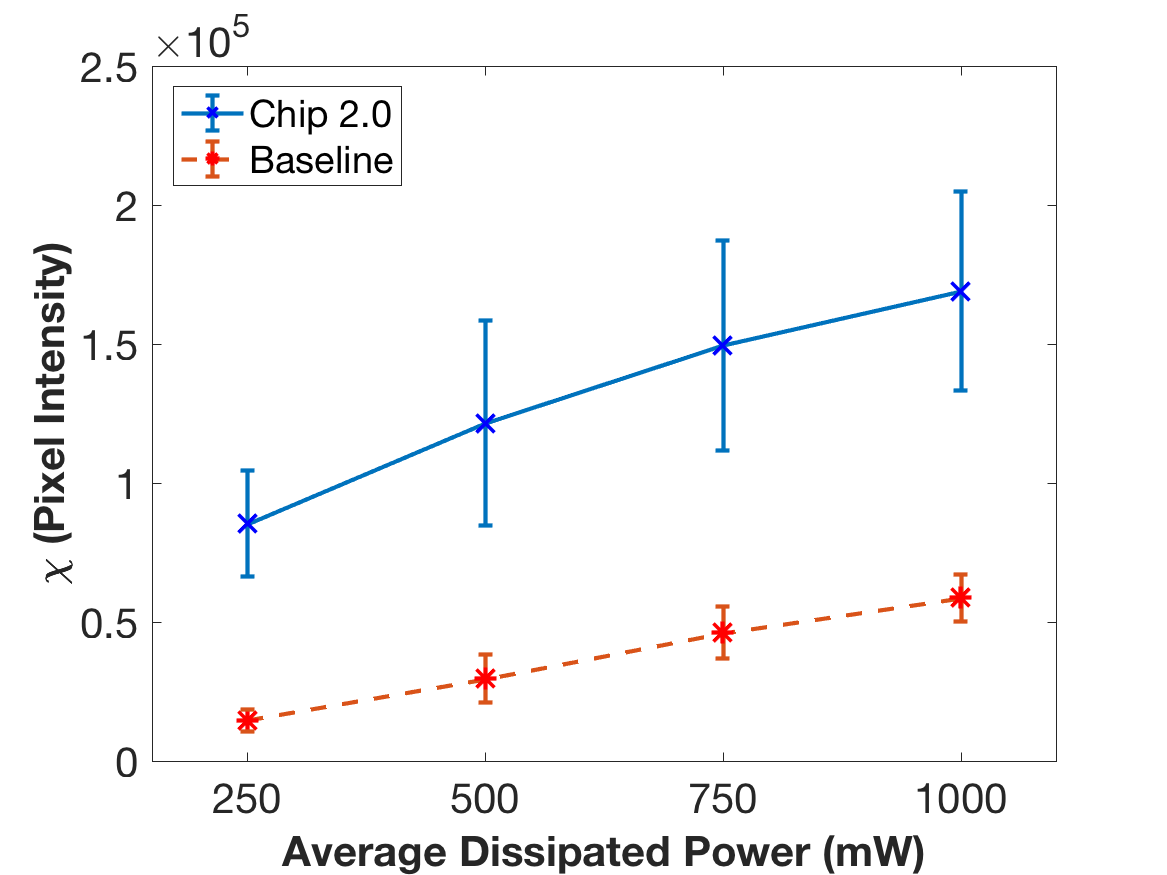
\includegraphics[width=7cm]{ErrorBars50ul}
    \medskip
    \centerline{(b) 50 $\mu$l/min}\\
  \end{minipage}
  \begin{minipage}[t]{0.99\linewidth}\centering
    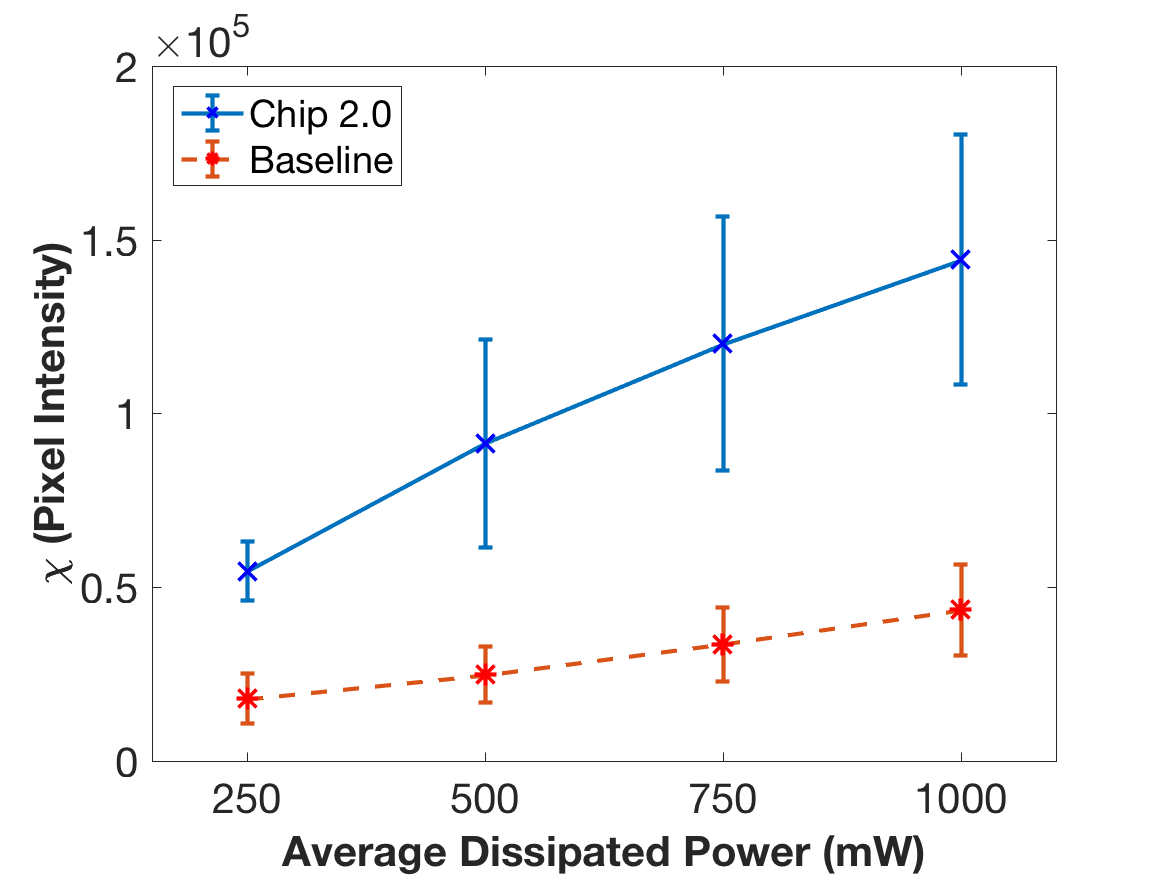
\includegraphics[width=7cm]{ErrorBars75ul}
    \medskip
    \centerline{(c) 75 $\mu$l/min}
  \end{minipage}
  \caption[Performance comparison versus baseline using image analysis]{Performance comparison versus baseline using image analysis. (a-c) plot the performance of the baseline versus the winner of the study for three volumetric flow rates: 25 $\mu$l/min, 50 $\mu$l/min and 75 $\mu$l/min, respectively. Performance is calculated from microscope images in the manner described in Section \ref{ssec:promToWidth}.}
	\label{fig:headToHeadImages}
\end{figure}


Figure \ref{fig:headToHeadImages}(a--c) plots the performance of Chip 2.0 against the baseline in terms $\chi$. The results show that Chip 2.0 outperforms the baseline for all tested combinations of flow and power settings.
\subsubsection{Comparative Blood Separation}
\label{sssec:comparisonBlood}

\begin{figure}[H]
  \begin{minipage}[t]{0.49\linewidth}\centering
    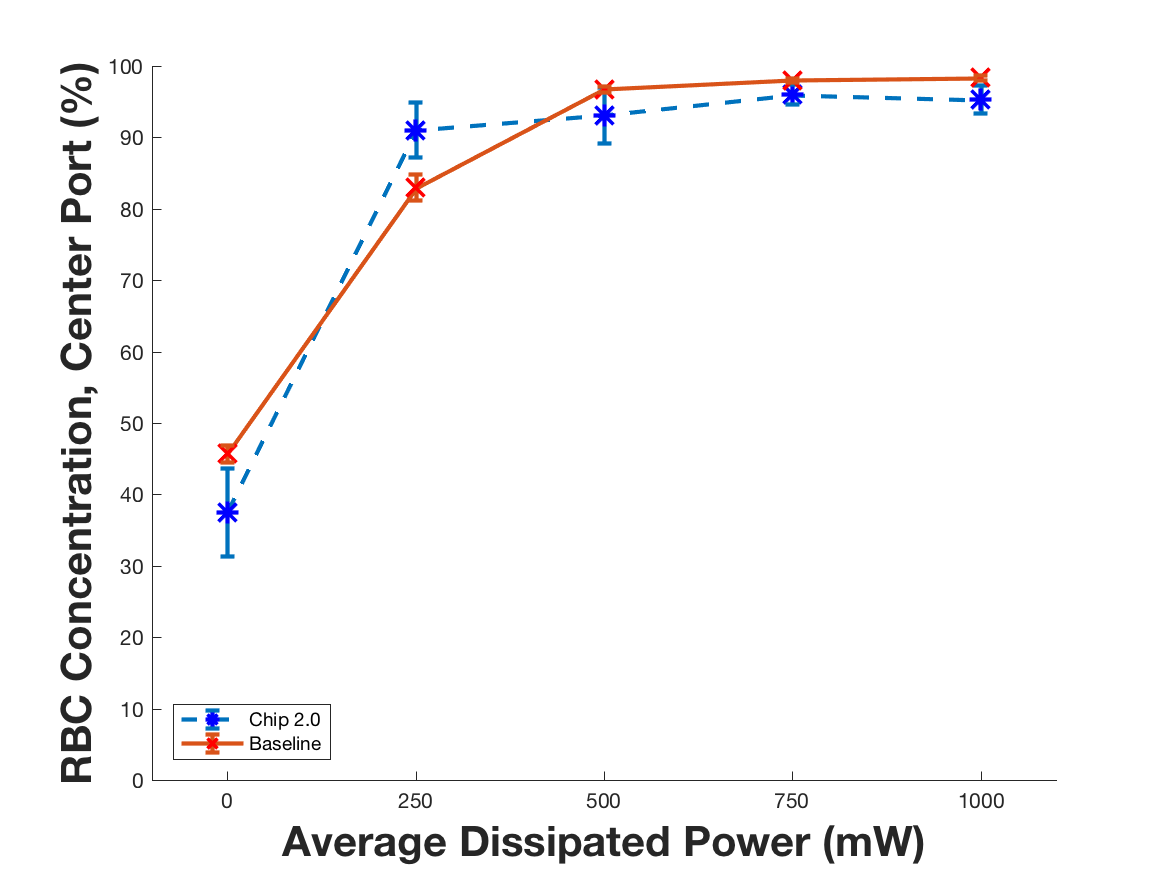
\includegraphics[width=7cm]{ErrorBarBloodData25ul}
    \medskip
    \centerline{(a) 25 $\mu$l/min}
  \end{minipage}\hfill
  \begin{minipage}[t]{0.49\linewidth}\centering
    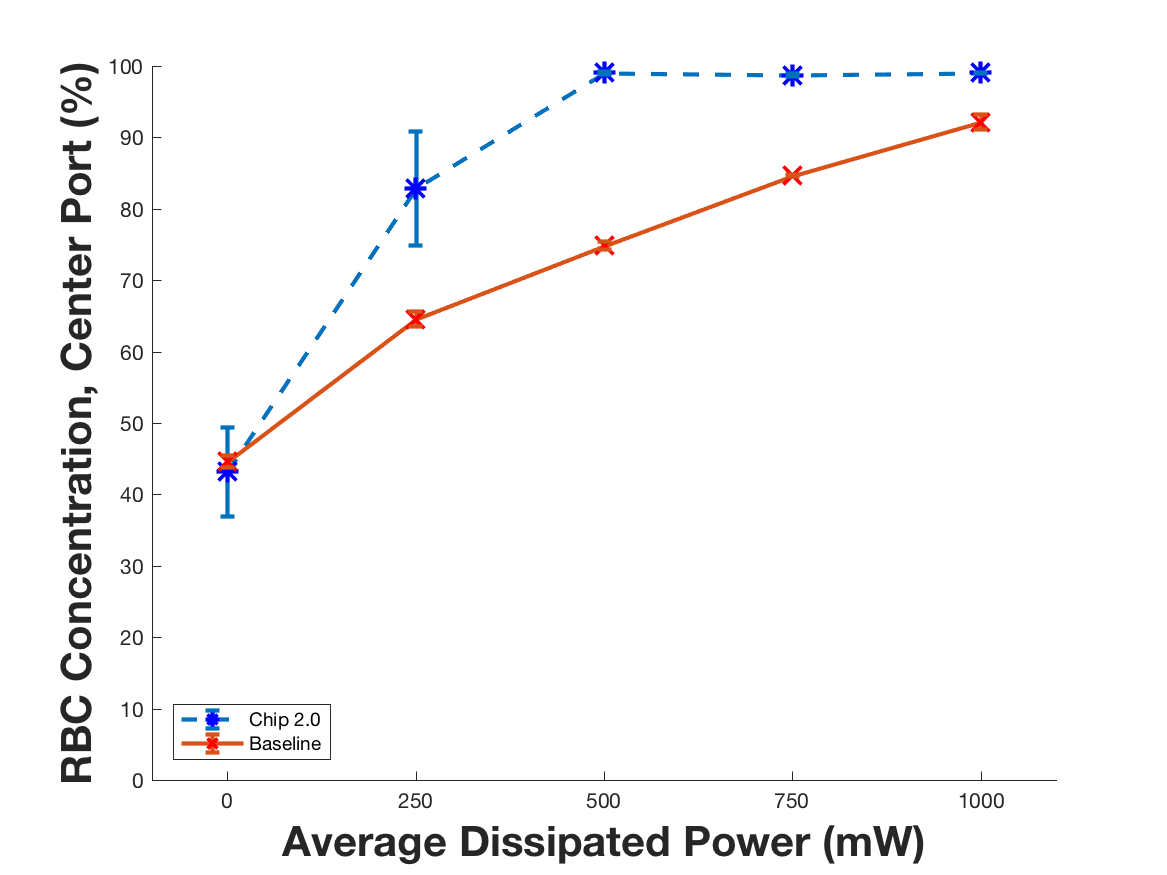
\includegraphics[width=7cm]{ErrorBarBloodData50ul}
    \medskip
    \centerline{(b) 50 $\mu$l/min}\\
  \end{minipage}
  \begin{minipage}[t]{0.99\linewidth}\centering
    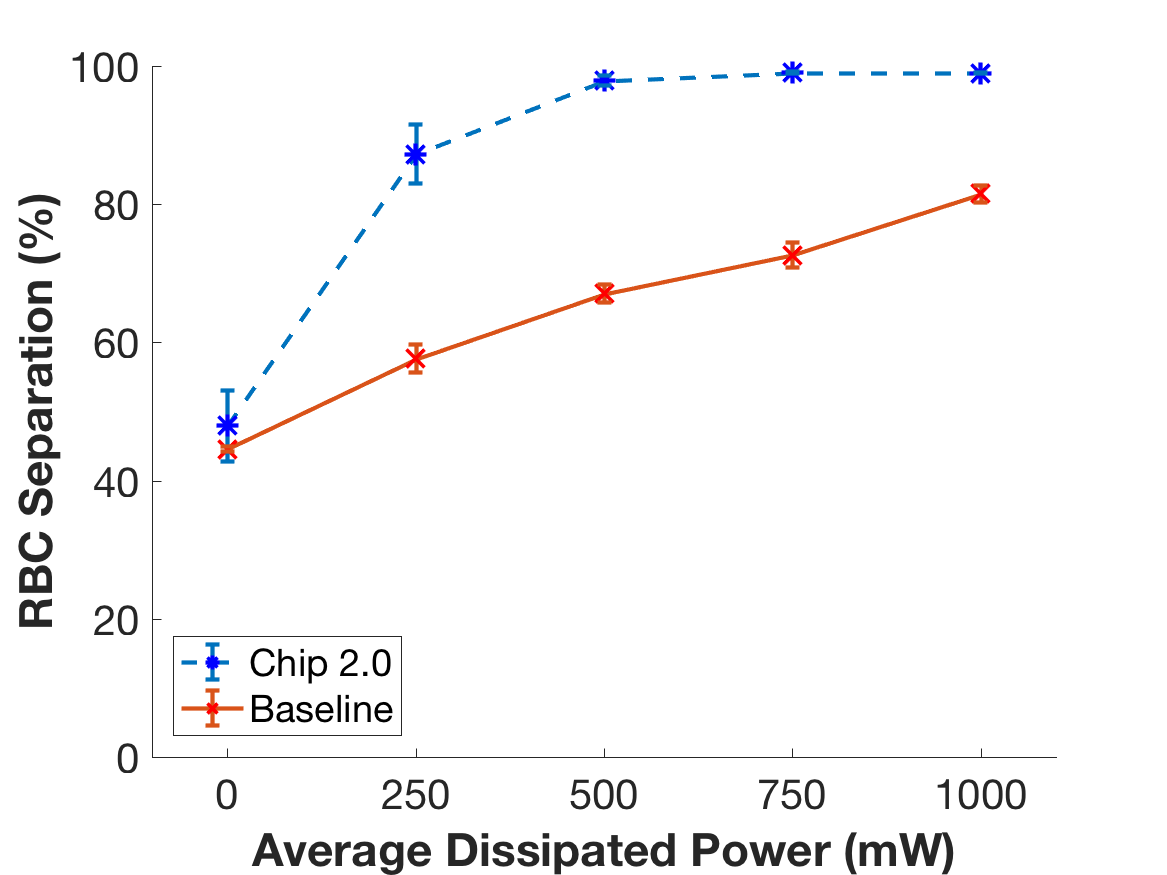
\includegraphics[width=7cm]{ErrorBarBloodData75ul}
    \medskip
    \centerline{(c) 75 $\mu$l/min}
  \end{minipage}
  \caption[Separation performance comparison versus baseline]{Blood separation performance comparison versus baseline. (a-c) plot the performance of the baseline versus the winner of the study for three volumetric flow rates: 25 $\mu$l/min, 50 $\mu$l/min and 75 $\mu$l/min, respectively. Performance is defined based on each design's ability to focus RBCs into the middle channel of the trifurcation shown in Figure \ref{fig:geometry}. RBC separation is defined as the number of RBCs measured at the center port divided by the total number of RBCs measured at the input port.}
	\label{fig:headToHeadBlood}
\end{figure}


Figure \ref{fig:headToHeadBlood} plots the performance of Chip 2.0 against the baseline in terms of each device's ability to focus RBCs to the center port. The dynamic range of each measurement was limited between the control measurement (i.e., zero average dissipated power) and 100\% RBC concentration in the center channel. As the chip has two outlet ports (Figure \ref{fig:geometry}), RBCs will be approximately equally distributed between them in the acoustics-off (0 W input power) condition. The baseline and Chip 2.0 demonstrated comparable performance at a flow rate of 25 $\mu$l/min across all power settings; however, at higher flow rates Chip 2.0 outperformed the baseline across all non-control power settings. 



\subsubsection{Comparative Bacterial Separation}
\label{sssec:comparisonBacteria}

Four experiments were conducted in three technical replicates, two for each device design (baseline and Chip 2.0),  in order to determine the optimal value for each measure of merit while holding the other constant. Optimality was defined as the maximum flow rate or minimum power required to maintain at least 90\% RBC separation between the side and center ports while bacteria recovery in the side port was measured. 

The results in Figure \ref{fig:bacPerf} show that Chip 2.0 achieved a 175\% increase in throughput relative to the baseline. Additionally, Chip 2.0 was able to decrease the average dissipated power by 81.63\% when compared to that of the baseline geometry. The actual average RBC separation across all four experiments was 95.25\% ($\pm$1.89\%). The yield of the bacterial samples collected at the side port had a standard deviation of 0.05\%.  For both devices the yield of bacteria in the side port was 33.5\% ($\pm$3\%) after separation, showing that separation performance in the 2.0 design is equal to that of the baseline while enabling lower driving power and/or higher throughput.

\begin{figure}[H]
  \begin{minipage}[t]{0.49\linewidth}\centering
    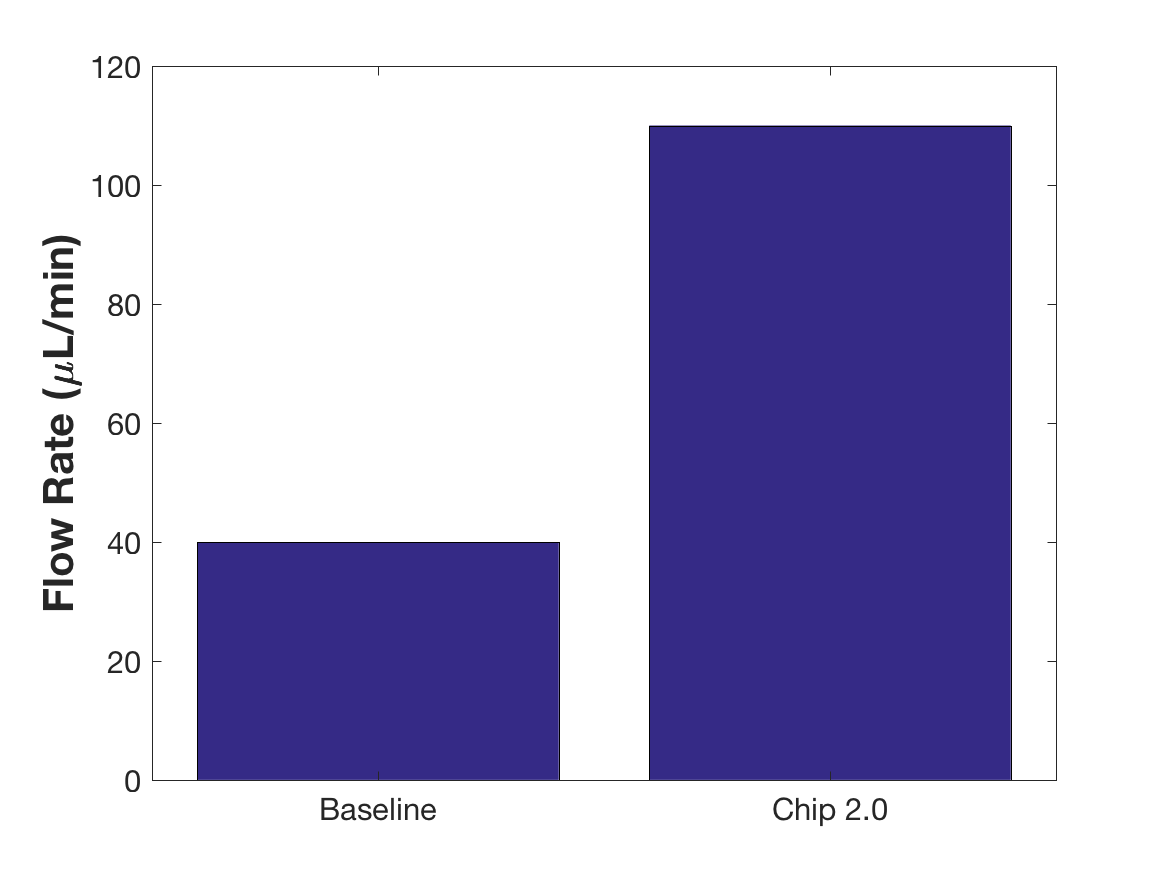
\includegraphics[width=7cm]{flowBac}
    \medskip
    \centerline{(a) Flow Rate at 1 W}
  \end{minipage}\hfill
  \begin{minipage}[t]{0.49\linewidth}\centering
    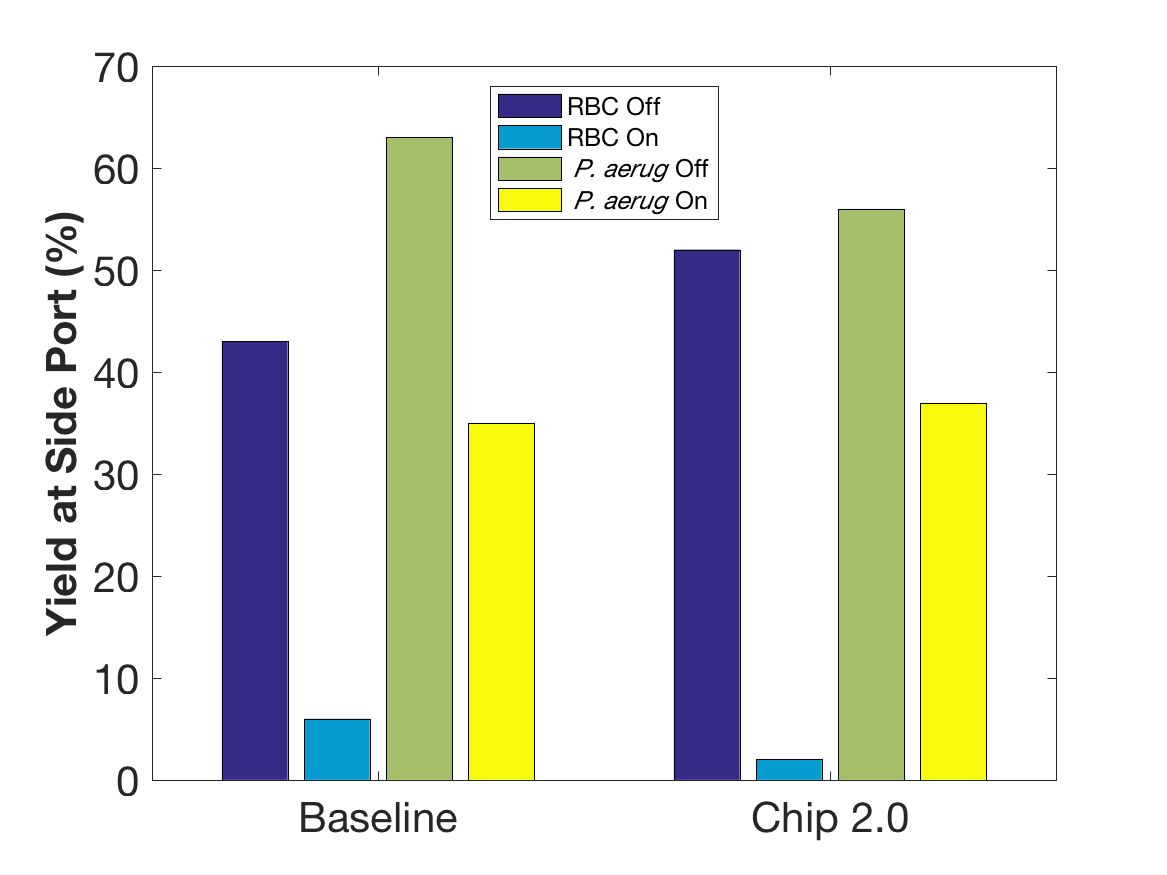
\includegraphics[width=7cm]{maxFlow}
    \medskip
    \centerline{(b) Separation performance for (a)}
  \end{minipage}\\
  \begin{minipage}[t]{0.49\linewidth}\centering
    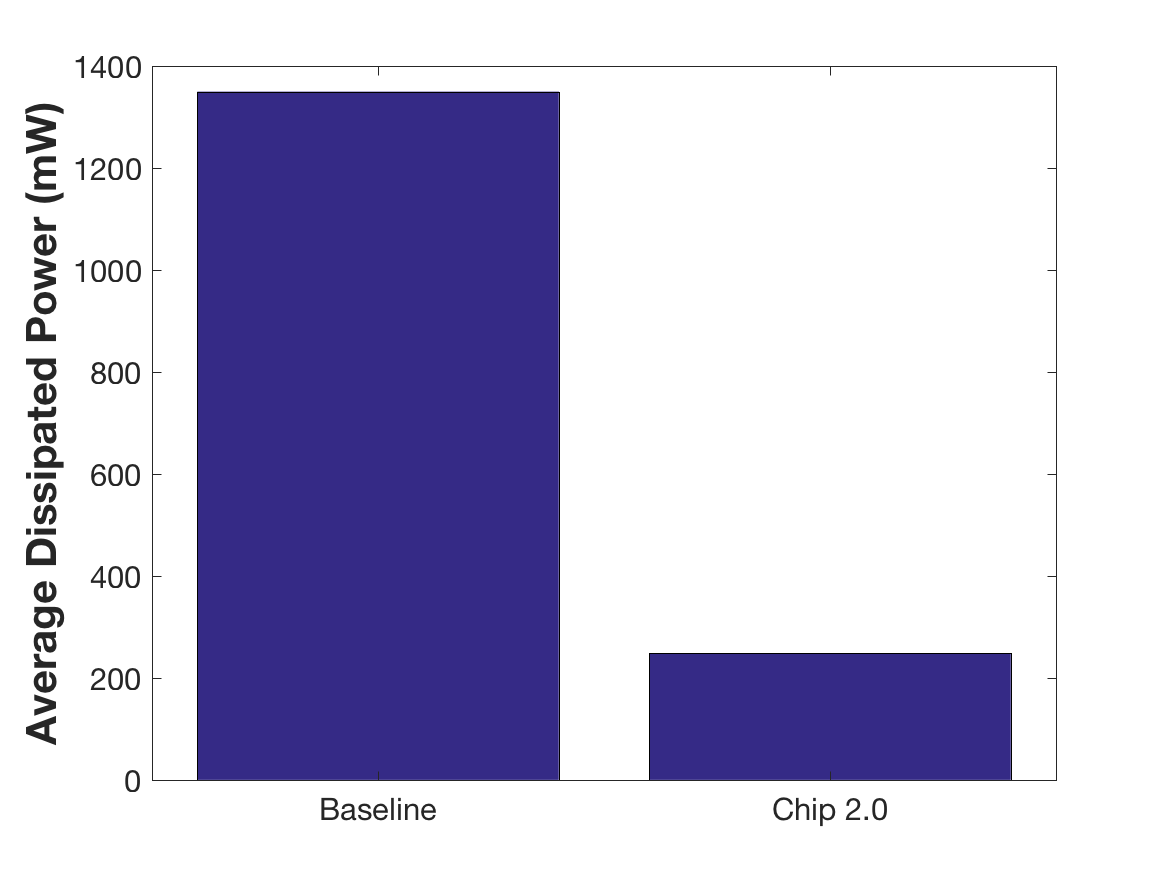
\includegraphics[width=7cm]{powerBac}
    \medskip
    \centerline{(c) Power at 50 $\mu$l/min}
  \end{minipage}\hfill
  \begin{minipage}[t]{0.49\linewidth}\centering
    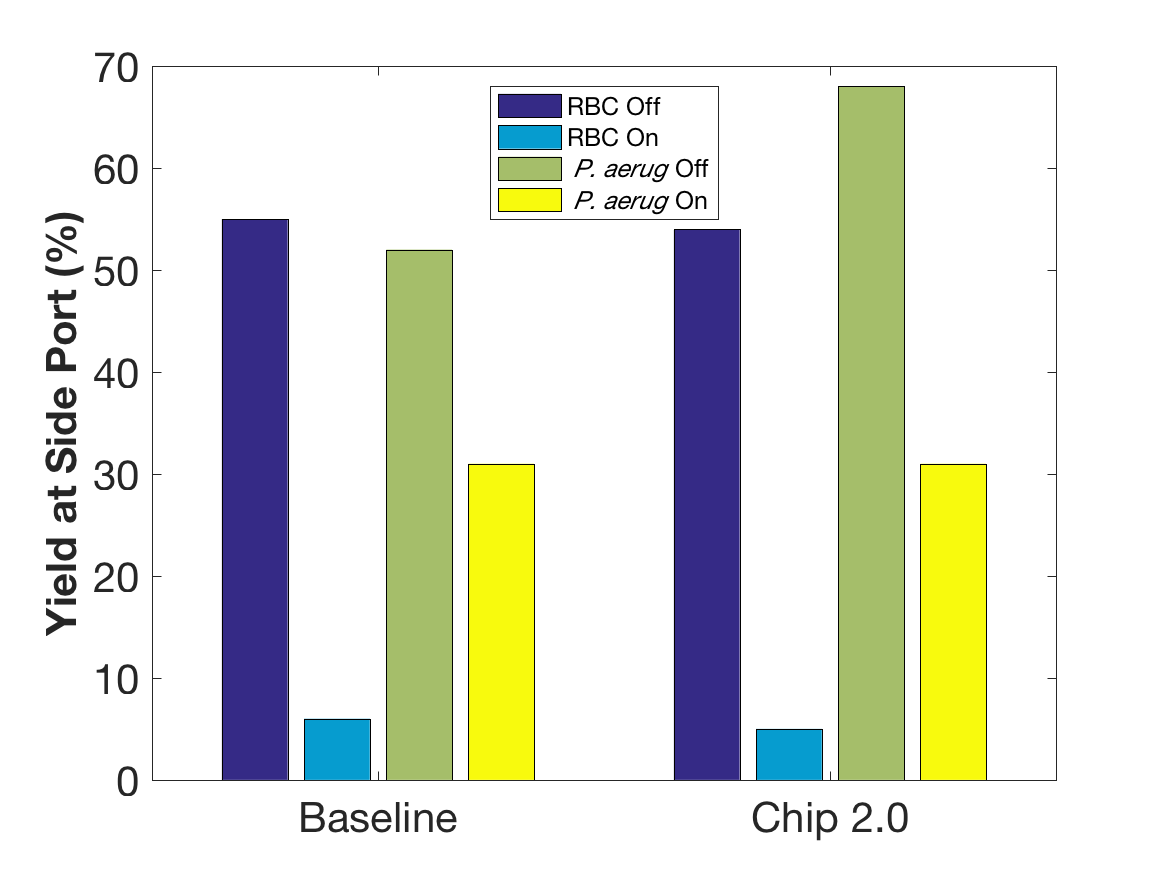
\includegraphics[width=7cm]{minPower}
    \medskip
    \centerline{(d) Separation performance for (b)}
  \end{minipage}\\
  \caption[Bacterial separation performance comparison]{Levels of each measure of merit required to achieve equivalent separation performance. (a) shows the relative performance of the baseline as it compares to Chip 2.0 in terms of flow rate with power held constant at 1 W. (b) illustrates the actual performance of each chip at the levels specified in (a) in both the acoustics ``off'' (0 W and established chip flow rate) and ``on'' conditions (1 W and established flow conditions). (c) summarizes the performance of the two chip designs holding flow rate at 50 $\mu$l/min while varying power. Constant values were maintained for RBC separation and bacterial recovery for all chip designs and experiments. (d) depicts the performance of each device at the power levels specified in (c); ``off'' being the control condition of 0 W and 50 $\mu$l/min.}
	\label{fig:bacPerf}
\end{figure}



It is worth noting that the Chip 2.0 design achieved better RBC separation  for both the maximum flow rate and minimum power experiments (98\% vs 94\% and 95\% vs 94\%, respectively) and equivalent bacterial recovery relative to the baseline across all four experiments; thus, for each Chip 2.0 experiment the measure of merit (flow or power) could show greater advantages if the RBC yield were adjusted to match that of the baseline. 

%Claim: without losing performance, we increased throughput and lowered power.

\section{Discussion}
\label{sec:discussion}

The resonant response of acoustophoretic microfluidic devices has been shown to be non-linear \cite{garofalo2016performance}\cite{bora2015efficient}\cite{glynne2009new}\cite{hahn2014modeling}. Complex response patterns with numerous explanatory variables have been successfully optimized using a fractional factorial experimental design approach in conjunction with a response surface methodology \cite{khuri2010response}; however, these methodologies assume that the function $f(x)$ modeling the response variable $y$ to the explanatory variables $x=(x_1,x_2,\dots,x_n)$ accounting for some experimental error $\epsilon$, as shown in Equation \ref{eqn:response}, is a low-degree polynomial \cite{khuri2010response}, 

\begin{equation}
\label{eqn:response}
  \hfill y=f(x)+\epsilon \hfill
\end{equation}

In the absence of a near-quadratic response, multiple rounds of experiments are required to adequately detect a positive gradient in performance \cite{carley2004response}. Even after multiple rounds of experiments, the nature of a complex response surface means that no claim of optimality can be made \cite{box2006improving}. Since this study seeks a performance enhancement, as opposed to a rigorous optimal geometry, this iterative method is acceptable.   

This study successfully improved the performance of the acoustic separator chip for both measures of merit. However, Chip 2.0 may not represent an optimal design, and further improvement is likely possible.  The experimental design selected parameters that were most accessible to systematic variation.  For example, the impact of total height of the device was not explored because changes in sheet stock thickness would require sourcing or custom fabricating those sheets, and the bond process would have to be adjusted for each thickness.  Likewise, the selection of the values tested assumes a more or less smoothly varying response.  Further analysis is needed to rigorously support that assumption.   

The frequency range studied for the rapid screening tests (0.5 -- 2.0 MHz) was chosen based on the known resonance of the baseline device (approximately 1 MHz) and the expectation that small variations in dimensions should result in comparably small variations in resonant frequency.  Additionally, the lower limit was selected with the knowledge that acoustic radiation force scales with frequency and lower frequencies could limit the ability of the device to focus small cells or particles such as platelets or bacteria, if desired in other applications.  Furthermore, there were practical experimental limitations at the upper end of the range; a transducer with a higher resonant frequency (ex., 5 MHz) would allow a wider range of frequencies to be explored, however the fragility of such transducers increases the difficulty of mounting and testing the devices.  Nevertheless reproducing the screening with a wider frequency range, particularly at the low end could yield further improvements.


Despite these and other limitations, this study was meant not only to identify an improved geometry, but also to establish a method for empirical development of devices.  The resulting performance improvement, as measured by the bacteria separation task, suggest that the initial screening using only image-based analysis of RBC focusing provides a useful approach for assessing devices.  To perform the setup, operation, output sample collection, and cell counting in the final bacteria separation takes several hours at least with all parameters fixed, whereas hundreds of image-based prominance measurements could be made at a rate of one every 15 seconds. 

Future explorations of device designs can be enabled by this parametric, rapid prototyping framework, which is part of a larger workflow \cite{ali2017iwbda}\cite{lippai2017iwbda}\cite{krishna2017iwbda}. The 19 devices designed in this manuscript can take advantage of this process with a high level description of the device functionality, microfluidic primitives, and automated fabrication and control.

%The accuracy of the desktop micromill ($<$0.003" per 6" of linear travel \cite{othermill}) as well as the centerline deviation (TIR) of the tools used to machine the chips all functioned within published parameters. This was confirmed using a calibrated microscope and drop gauge (\textbf{\uppercase{I need to grab the model number from the machine shop}}). YOU CAN TAKE THIS OUT OR MOVE TO METHODS

%Finally, many unstudied parameters exist upon which another optimization effort can be conducted. As this study only used one type of transducer, one can imagine another study sweeping across the mechanical quality factor ($Q_m$), resonant frequency, size, or material of the piezoelectric transducer. Additionally, other parameters inherent to the fluidic device were left unstudied, such as the total device thickness or channel widths after the trifurcation.  I AM GOING TO SUGGEST WE LEAVE THE TRANSDUCER OUT OF THIS, SO LETS SKIP THIS PARAGRAPH

\section{Conclusion}
\label{sec:conclusion}
Enabled by a parametric, rapid prototyping framework, we were able to screen 19 device designs, distinct in four geometric parameters, towards optimizing the performance of a blood-bacteria separation device. Compared to the previously published plastic design, we demonstrate that the optimized device geometry can separate blood and bacteria while operating at 175\% greater flow rate as well as reducing the power requirement by 81.63\% for equivalent separation performance.   The improved device will offer increased throughput and reduced power requirements and could aid performance of future point-of-care plastic acoustofluidic devices.

\cleardoublepage


% -------------------------------------
% CHAPTER 2: THE BODY OF THESIS
% -------------------------------------
%\chapter{Body of my thesis}
\label{chapter:body}
\thispagestyle{myheadings}

% set this to the location of the figures for this chapter. it may
% also want to be ../Figures/2_Body/ or something. make sure that
% it has a trailing directory separator (i.e., '/')!
\graphicspath{{2_Body/Figures/}}

\section{Some results}
\label{sec:your_face_results}

Here goes all the important stuff, likely with a lot of graphics like this:

\begin{figure}[htb]
  \begin{minipage}[t]{0.49\linewidth}\centering
    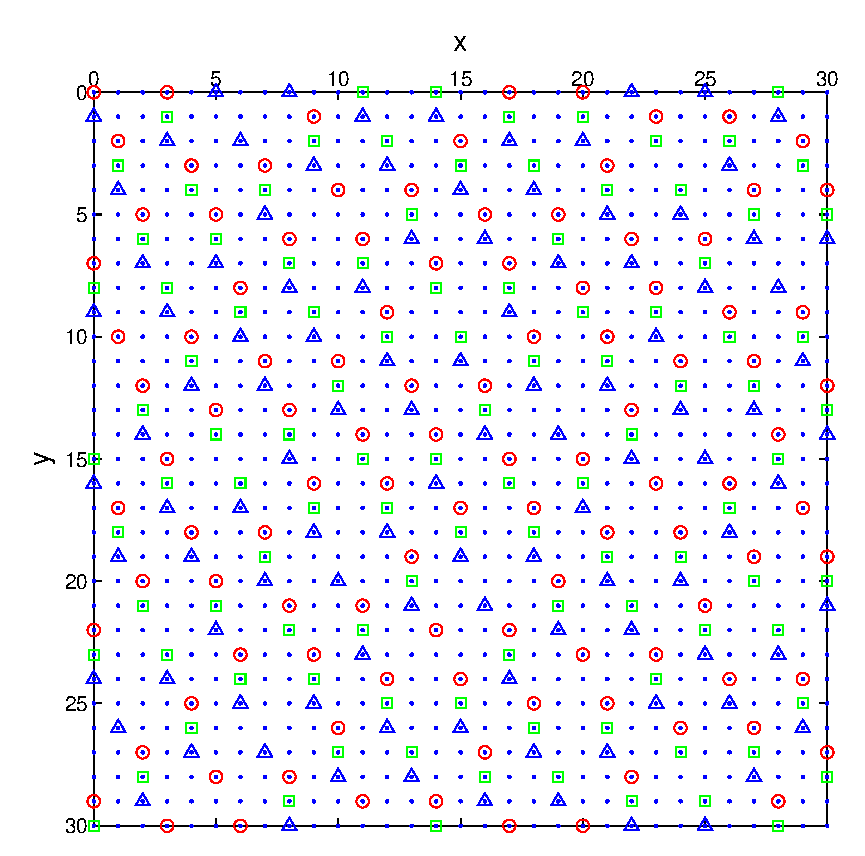
\includegraphics[width=7cm]{figure_sampling_view1.eps}
    \medskip
    \centerline{(a)}
  \end{minipage}\hfill
  \begin{minipage}[t]{0.49\linewidth}\centering
    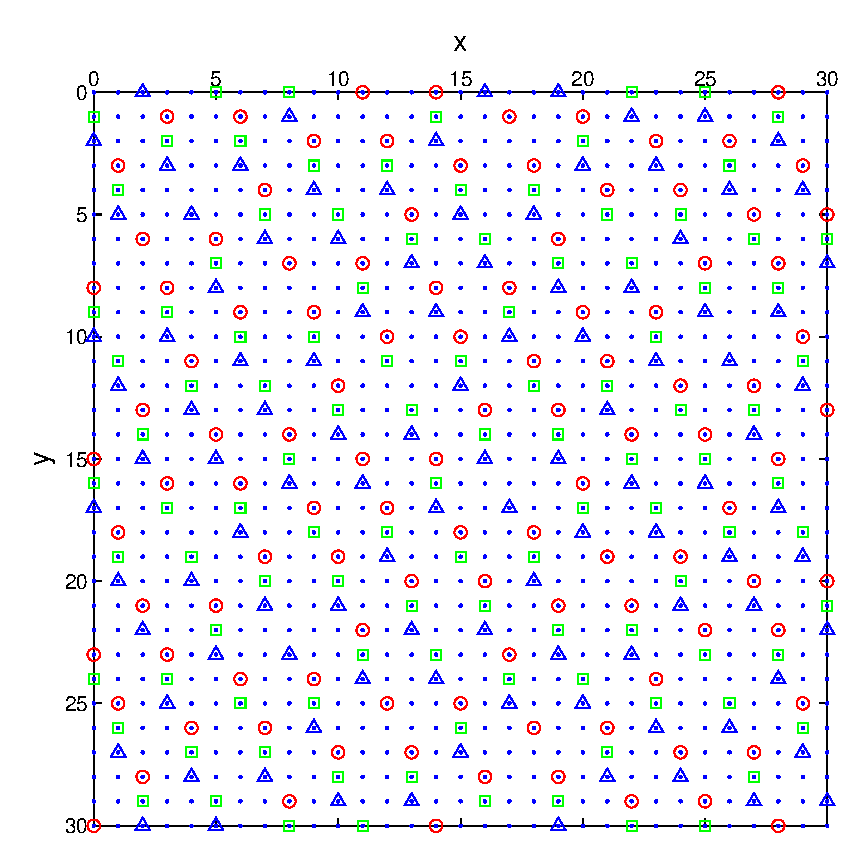
\includegraphics[width=7cm]{figure_sampling_view2.eps}
    \medskip
    \centerline{(b)}
  \end{minipage}
  \caption{Assignment of single-view intensities to RGB components: (a) view
    \#1; and (b) view \#2. }
  \label{fig:Sampling}
\end{figure}

You will also be using a lot of citations. Here is the format required in the dissertation: \cite{lamport1985:latex},\cite{Debr01}.

In all likelihood, you will need to insert tables. See one example on the next page.
\clearpage

\begin{table}[h]
	\caption{Absolute disparity error per pixel for the test data from
		Fig.~\ref{fig:Sampling} and different parameter values. In each experiment one
		parameter is adjusted while other parameters are unchanged.} 
	\centering
	\begin{minipage}[b]{0.30\linewidth}
		\centerline{$\eta=6000$, $\mu=2000$}\smallskip
		\centering
		\begin{tabular}{ccc}
			\hline
			$K$ & $u_1$ & $u_2$\\
			\hline
			3   & 0.52 &0.46\\
			7   & 0.47 &0.43\\
			10  & 0.35 &0.36\\
			12  & 0.37 &0.36\\
			\hline
		\end{tabular}
	\end{minipage}
	%
	\begin{minipage}[b]{0.34\linewidth}
		\centerline{$K=10$, $\mu=2000$}\smallskip
		\centering
		\begin{tabular}{ccc}
			\hline
			$\eta$ & $u_1$ & $u_2$\\
			\hline
			1000&0.54& 0.45\\
			3000&0.43& 0.40\\
			6000&0.35& 0.36\\
			9000&0.37& 0.37\\
			\hline
		\end{tabular}
	\end{minipage}
	%
	\begin{minipage}[b]{0.32\linewidth}
		\centerline{$K=10$, $\eta=6000$}\smallskip
		\centering
		\begin{tabular}{ccc}
			\hline
			$\mu$ & $u_1$ & $u_2$\\
			\hline
			100 &1.00&1.16\\
			1000&0.53&0.47\\
			2000&0.35&0.36\\
			3000&0.44&0.43\\
			\hline
		\end{tabular}
	\end{minipage}
	%
	\label{tab:Parameters}
\end{table}

Of course, there must be a Table of Contents at the beginning of the thesis.

%\cleardoublepage

% -------------------------------------
% CHAPTER 3: CONCLUSION
% -------------------------------------
\chapter{Conclusions and Future Work}
\label{chapter:Conclusions}
\thispagestyle{myheadings}

% set this to the location of the figures for this chapter. it may
% also want to be ../Figures/2_Body/ or something. make sure that
% it has a trailing directory separator (i.e., '/')!
\graphicspath{{3_Conclusion/Figures/}}

One major goal of this thesis was to lower the barrier of entry into the field of continuous flow microfluidics. This was achieved by developing a rapid, cost-effective, CAD-friendly, design-to-fabrication framework for microfluidics using accessible CAM technologies such as desktop CNC mills and 3D printers. Proving the efficacy of this framework involved demonstrating its capacity to solve relevant and complex experimental problems. The scalability of the framework was proven by its ability to design, fabricate, and control a complex network of novel microfluidic primitives, as shown in Chapter \ref{chapter:xposer}. Its experimental relevance was established in Chapter \ref{chapter:acoust} by optimizing an acoustofluidic blood--bacteria separation device in a thermoplastic substrate --- something that has never been done before.

Having demonstrated this new rapid prototyping framework is capable of designing, fabricating, and controlling complex and experimentally relevant devices, the next logical step would be to bring this research back to its genesis. This work was motivated by the desire to orchestrate large networks of novel synthetic biological systems. I presented a framework capable of designing a device that separates smaller genetic logic components into disparate reaction chambers and connecting these chambers using microchannels, through which biological signals can be sent. My framework provides a mechanism to describe and execute temporally specified valve control sequences, which can control the flow of biological signaling information such that larger functionality can be achieved. 

Additionally, the state of the genetic circuits can be monitored using on-chip diagnostics such as the integration of sensors and optical reporting areas. This on-chip feedback can be integrated into the temporal valve-control specification, thus necessitating an extension to the Biostream language beyond ``wait'' and ``set'' statements to include some element of temporal logic such as ``wait until''.

All of these extensions should be fully integrated into the larger CAD workflow shown in Figure \ref{fig:fullflow}. This would require forgoing the use of OpenSCAD and replacing it with domain-specific CAD tools such as Fluigi Place and Route \cite{hu2014} using MIcrofluidic NeTlist \cite{krishna2017iwbda} descriptions. Smaller devices could be designed using a microfluidic-specific drawing tool such as 3D$\mu$F \cite{lippai2017iwbda}. All designs could be informed by a design-automation platform driven by fluid mechanics \cite{ali2017iwbda}, which would provide aspects of automation to device parameter estimation. The design tools listed are compatible with MakerFluidics in that they can export two-dimensional graphics files (i.e., SVG files), however these tools could be extended to output designs in three dimensions. It must be noted that all of the preceding design tools are made relevant by the ability to fabricate the designs they create; this relevance is boosted by the accessibility MakerFluidics brings to continuous-flow microfluidics.


My results show that low-cost microfluidic fabrication techniques are possible and relevant. The integration of continuous-flow microfluidics into day-to-day life in a typical wet lab has the ability to change the way experimentalists look at the nature of their work. Freed from the mundane and costly burdens of device design, fabrication, and running protocols, experimentalists could spend more time on data analysis and experimental documentation --- effectively boosting the quality and quantity of research. MakerFluidics and the capabilities it enables represent an important step towards this integration.

\cleardoublepage

%\appendix
\begin{appendices}
\chapter{Proof of xyz}
\label{appendix}
\thispagestyle{myheadings}

This is the appendix.
\end{appendices}
%==========================================================================%
% Bibliography
\newpage
\singlespace
\bibliographystyle{apalike}

% each subdirectory can have its own BiBTeX file
\bibliography{thesis,mf,sb,ece}
\cleardoublepage

%==========================================================================%
% Curriculum Vitae
\addcontentsline{toc}{chapter}{Curriculum Vitae}

{\centering
\Large
\textbf{Ryan Silva}

\normalsize
8 St. Mary's St.

PHO 209

Boston University

Boston, MA 02215

rjsilva@bu.edu\\[1cm]
}
\large
\textbf{Education}\\
\rule{\textwidth}{1pt}

\begin{table}[h!]
\centering
\small
\begin{tabular}{ p{9.5cm} p{2.5cm} p{4.5cm}}
	\multicolumn{3}{l}{\textbf{Boston University, Boston, MA 02215}}\\
	PhD, Electrical and Computer Engineering & GPA: 4.0/4.0 & 2014 - 2017\\
	\multicolumn{3}{l}{\textbf{Advisor: }Douglas Densmore}\\
	\multicolumn{3}{l}{\textbf{Thesis: }Exploring the Boundaries of Computer Engineering, Biology and Microfluidics}\\
	 & & \\
	\multicolumn{3}{l}{\textbf{Air Force Institute of Technology (AFIT), Dayton, OH, 45433}}\\
	Master of Engineering, Electrical Engineering & GPA: 3.8/4.0 & 2005 - 2007\\
	\multicolumn{3}{l}{\textbf{Advisor: }Rusty Baldwin}\\
	\multicolumn{3}{l}{\textbf{Thesis: }Optimizing the Advanced Encryption Standard for an 8-bit Datapath}\\
	 & & \\
	\multicolumn{3}{l}{\textbf{United States Air Force Academy (USAFA), Colorado Springs, CO, 80841}}\\
	Bachelor of Science, Electrical Engineering & GPA: 3.7/4.0 & 2002 - 2005\\
\end{tabular}
\end{table}

\large
\textbf{Awards}\\
\rule{\textwidth}{1pt}

\begin{table}[h!]
\centering
\small
\begin{tabular}{ p{12.5cm} p{4.5cm}}
	Charles Stark Draper Laboratory Fellow & 2016 - 2017 \\
	USAFA Faculty Pipeline Fellow & 2014 - 2017 \\
	Great Minds in STEM Most Promising Engineer & 2013 \\
	IEEE Design Excellence Award & 2013 \\
	Outstanding Academy Educator & 2013
\end{tabular}
\end{table}

\large
\textbf{Professional Affiliations}\\
\rule{\textwidth}{1pt}

\begin{table}[h!]
\centering
\small
\begin{tabular}{ p{12.5cm} p{4.5cm}}
	Association for Computing Machinery VLSI (ACMVLSI) & Reviewer 2017 \\
	American Society of Engineering Education (ASEE) & Member 2011 \\
	Tau Beta Pi - National Engineering Honor Society & Inducted 2006\\
	Eta Kappa Nu - National Electrical Engineering Honor Society & Inducted 2006\\
	Institute of Electrical and Electronics Engineers (IEEE) & Member 2004 \\
	United States Air Force Academy Association of Graduates (USAFA AOG) & Member 2001
\end{tabular}
\end{table}

\large
\textbf{Invited Talks}\\
\rule{\textwidth}{1pt}

\small
\begin{itemize}
	\item ``\textit{MakerFluidics: Microfluidics for the Masses}'' \\2nd Workshop on Molecular Communications\\Dublin, Ireland 9 May 2017
\end{itemize}

\large
\textbf{Publications}\\
\rule{\textwidth}{1pt}

\small
\begin{enumerate}
	\item{R. Dubay, \textbf{R. Silva} and J. Fiering, ``High Throughput Acoustophoresis in an Array of Parallel Plastic Microchannels'' Acoustofluidics 2017.}
	\item{\textbf{R. Silva}, P. Dow, R. Dubay, C. Lissandrello, J. Holder, D. Densmore and J. Fiering, ``Rapid prototyping and parametric optimization of plastic acoustofluidic devices for blood--bacteria separation'' Biomedical Microdevices 2017.}
	\item{\textbf{R. Silva}, S. Bhatia, and D. Densmore, ``A reconfigurable continuous-flow fluidic routing fabric using a modular, scalable primitive,'' Lab on a Chip 2016.}
	\item{\textbf{R. Silva}, R. Sanka and D. Densmore, ``MakerFluidics: Microfluidics for the Masses'' Eighth International Workshop on Bio-Design Automation (IWBDA) 2016.}
	\item{\textbf{R. Silva}, A. Heuckroth, H. Huang, A. Rolfe and D. Densmore, ``MakerFluidics: Microfluidics for All'', SynBERC 2015.}
	\item{P. Vaidyanathan, B. Der, S. Bhatia, N. Roehner, \textbf{R. Silva}, C. Voigt and D. Densmore, A Framework for Genetic Logic Synthesis. Proceedings of the IEEE 2015.}
	\item{H. Huang, A. Heuckroth, \textbf{R. Silva}, S. Bhatia, and D. Densmore, ``Fluigi: An Automated Framework for Creating Bioelectronic Devices", Seventh International Workshop on Bio-Design Automation (IWBDA), 2015.}
	\item{A. Pacheco, \textbf{R. Silva}, S. Iverson, T. Haddock and D. Densmore, ``Multicellular Logic through Conversion of Genetic Circuit Outputs into Electrical Signals'', SynBERC 2015.}
	\item{A. Heuckroth, H. Huang, \textbf{R. Silva}, S. Iverson, T. Haddock, A. Pacheco, and D. Densmore, ``Accessible microfluidic mold fabrication using 3d printing", SynBERC 2015.}
	\item{C. Hendrix, D. Neebel and \textbf{R. Silva}, A Breadth First Course in Electrical and Computer Engineering. ASEE 2014.}
	\item{M. Roberts, R. Deppensmith and \textbf{R. Silva}, Observations from First-Year Instructors: What We Wish We Knew Before We Began. ASEE 2012.}
	\item{\textbf{R. Silva}, ``Implementation and Optimization of the Advanced Encryption Standard Algorithm using an 8-bit Datapath'', Defense Technical Information Center 2007.}
\end{enumerate}

\newpage

\large
\textbf{Teaching Experience}\\
\rule{\textwidth}{1pt}

\begin{table}[h!]
\centering
\small
\begin{tabular}{ p{12.5cm} p{4.5cm}}
	\textbf{United States Air Force Academy}, Assistant Professor of ECE& \\
ECE382 Embedded Systems I, Course Director& AY2012-2014\\
ECE281 Digital Design and Computer Architecture, Course Director & AY2012-2014\\
ECE210 Principles of Air Force Electronic Systems(Maj), Course Director & AY2013-2014\\
ECE315 Principles of Air Force Electronic Systems(Core), Instructor & AY2011-2013\\
ENGR101 Introduction to Air Force Engineering, Instructor & AY2012-2014\\
ECE463/464 Capstone Design Project, Mentor & AY2012-2014
\end{tabular}
\end{table}



 

%==========================================================================%
\end{document}
